\documentclass[a4paper,10pt]{ltjsarticle}
\usepackage[margin=22mm]{geometry}
\usepackage{amsmath,graphicx,booktabs,siunitx,hyperref,float,tikz,caption}
\usepackage[section]{placeins}
\usetikzlibrary{arrows.meta,positioning}
\hypersetup{colorlinks=true,urlcolor=blue,linkcolor=blue}
\graphicspath{{../experiments/figures/overview/}}
\newcommand{\plot}[3]{\begin{figure}[htbp]\centering\includegraphics[width=#2\linewidth]{#1.pdf}\caption{#3}\end{figure}}
\title{\sffamily ロボコンの操縦通信とWi-Fi干渉の可視化\\室内通信実験と先行SDR観測の統合}
\author{貝淵蒼馬}
\date{}
\newcommand{\maybeplot}[3]{\IfFileExists{../experiments/figures/receiver/#1.pdf}{\plot{#1}{#2}{#3}}{}}

\usepackage{luatexja-fontspec,titlesec}
\setsansfont{HaranoAjiGothic-Medium.otf}[BoldFont=HaranoAjiGothic-Medium.otf]
\setsansjfont{HaranoAjiGothic-Medium.otf}[BoldFont=HaranoAjiGothic-Medium.otf]
\titleformat{\section}{\Large\bfseries\sffamily}{\thesection}{1em}{}
\titleformat{\subsection}{\large\bfseries\sffamily}{\thesubsection}{1em}{}
\usepackage{adjustbox}
\begin{document}
\maketitle
\begin{abstract}
ロボコンで操縦指令・映像・点群がWi-Fiを共有し、他チームも通信する状況を室内で評価した。同一・隣接・分離チャネルと20/40 MHz幅、Wi-Fiと独立BLE通信、流量・生成周期、実ROS 2 Humble／JazzyのImage／PointCloud2のQoS、省電力設定、ESP-NOWの指令周期を比較する。構成の異なる342通信試行と115受信観測系列を区別して統合し、実測青緑SDR画像と応答期限・欠落・更新途絶を対応づける。ESP-NOW長時間系列は各600秒の19試行で、使用者の終了希望により残り5試行を省略した。実ロボット・実センサは用いていない。
\end{abstract}
\newcommand{\SameIdlePninetyNine}{10.6}
\newcommand{\SameTwentyPninetyNine}{21.0}
\newcommand{\SameHighPninetyNine}{36.9}
\newcommand{\SameHighDeadline}{7.4}
\newcommand{\SameHighGap}{102.9}
\newcommand{\VideoHighRange}{38.4--40.6}
\newcommand{\Conditions}{56}
\newcommand{\ControlPackets}{168000}
\newcommand{\Snapshots}{34320}
\newcommand{\RailMax}{0.0000}
\newcommand{\DutyRatio}{0.418}
\newcommand{\SendJitterRange}{1.06--1.98}
\newcommand{\SixPninetyNine}{26.5}
\newcommand{\SixDeadline}{1.8}
\newcommand{\SixLoss}{0.00}
\newcommand{\SixGap}{68.3}
\newcommand{\SevenPninetyNine}{15.6}
\newcommand{\SevenDeadline}{0.3}
\newcommand{\SevenLoss}{0.00}
\newcommand{\SevenGap}{40.4}
\newcommand{\ElevenPninetyNine}{13.1}
\newcommand{\ElevenDeadline}{0.2}
\newcommand{\ElevenLoss}{0.00}
\newcommand{\ElevenGap}{42.6}
\newcommand{\IdlePninetyNine}{10.8}
\newcommand{\IdleDeadline}{0.0}
\newcommand{\IdleLoss}{0.00}
\newcommand{\IdleGap}{33.0}
\newcommand{\WidthTwentyPninetyNine}{13.8}
\newcommand{\WidthTwentyDeadline}{0.2}
\newcommand{\WidthTwentyLoss}{0.00}
\newcommand{\WidthTwentyGap}{44.3}
\newcommand{\WidthFortyPninetyNine}{20.0}
\newcommand{\WidthFortyDeadline}{1.0}
\newcommand{\WidthFortyLoss}{0.00}
\newcommand{\WidthFortyGap}{62.6}
\newcommand{\LowPowerPninetyNine}{15.1}
\newcommand{\LowPowerDeadline}{0.2}
\newcommand{\LowPowerLoss}{0.00}
\newcommand{\LowPowerGap}{39.3}













% BEGIN TWO TEAM STUDY
% BEGIN OPERATIONAL STUDY
\section*{追加運用評価の実測と考察}

\section{流量制限の比較}

version7・source helper version2で新たに取得した45試行、15条件、各3反復・30秒。全135000指令送信、122665応答、25518 I/Q取得。全条件の数値検算・現行接続相手の応答確認・負荷設定readbackを確認し、図を目視した。旧version6の取得は非公開の予備診断記録として保存し、正式比較には混ぜない。

観測PCのAPはCh6・20 MHz、指令役ESP32からAPを経由してラップトップ2へ64 byte・100 HzのUDP指令を往復する。同じWi-Fiでラップトップ2から指令役へTCP模擬データを送る。他チームは独立したESP32 AP→STAに飽和TCPを要求する。ROS 2・実カメラ・実LiDARの試験ではない。配置は全機器が同じ机上、おおむね30 cmで固定。SDRボードはESP32-C5-WROOM-1。

\begin{center}\small\begin{adjustbox}{max width=\linewidth}
\begin{tabular}{llllll}\toprule
他チームCh & 自チーム要求TCP [Mbps] & 応答RTT統合p99 [ms] & 20 ms期限超過 [\%] & 自チーム実受信平均 [Mbps] & 他チーム実受信範囲 [Mbps]\\
\midrule
6 & 0 & 128.89 & 54.08 & 0.000 & 2.774–4.034\\
6 & 0.25 & 134.25 & 55.38 & 0.250 & 2.437–3.534\\
6 & 0.5 & 141.65 & 58.88 & 0.514 & 2.332–3.590\\
6 & 1 & 157.23 & 72.61 & 1.007 & 3.152–3.401\\
6 & 2 & 162.88 & 69.47 & 1.105 & 2.101–4.404\\
7 & 0 & 123.73 & 51.44 & 0.000 & 2.117–2.840\\
7 & 0.25 & 126.82 & 53.08 & 0.250 & 2.048–2.494\\
7 & 0.5 & 130.39 & 54.20 & 0.502 & 1.653–2.660\\
7 & 1 & 137.61 & 61.36 & 1.010 & 1.803–2.412\\
7 & 2 & 130.21 & 58.89 & 0.977 & 1.709–2.621\\
11 & 0 & 372.40 & 53.77 & 0.000 & 0.639–1.682\\
11 & 0.25 & 137.84 & 51.58 & 0.250 & 0.678–1.453\\
11 & 0.5 & 393.34 & 53.73 & 0.494 & 0.074–1.928\\
11 & 1 & 244.82 & 56.82 & 0.927 & 0.210–1.868\\
11 & 2 & 125.73 & 52.61 & 1.055 & 0.948–1.345\\
\bottomrule\end{tabular}\end{adjustbox}\end{center}

統合p99は戻った応答をまとめた分位点であり、各反復p99の平均ではない。20 ms期限超過は欠落を含む。各条件の環境反復数は3回であり、135000パケットを独立した環境反復と扱わない。図の小さい点で反復間の変動を併記する。

\section{自チームの大容量通信と指令品質}

要求0→1 Mbpsで期限超過率は、同一Ch6で54.08→72.61\%、隣接Ch7で51.44→61.36\%、分離Ch11で53.77→56.82\%となった。平均速度だけでは指令品質を表せない。Ch6・要求1 Mbpsの実受信は平均1.007 Mbpsだが、20 ms期限超過は72.61\%だった。この構成では画像・点群相当の通信を制限することが指令遅延を減らす候補になる。

ただし要求量に比例した単調な劣化ではない。要求2 Mbpsでは、全チャネルで実受信が要求に達せず、アプリ未送信byteが累積した。例えばCh6の実受信平均は1.105 Mbpsで、期限超過69.47\%は要求1 Mbpsより低い。これを「2 Mbpsの方が安全」と解釈できない。生成量、アプリの待ち行列、ソケットの受付、RFの送信機会、受信量は異なる観測であり、バックプレッシャーで負荷の形が変わる。

\section{チャネル分離の効果と比較の限界}

要求1 Mbpsにおける期限超過は同一Ch6、隣接Ch7、分離Ch11の順に低かった。ただし、他チームの実受信量もチャネルで異なり、同じ干渉電力・同じ空中時間を与えた比較ではない。机上固定でも受信量と端末状態は変動している。3反復の結果から会場全体に通用するチャネル順位や安全なMbps上限を決めない。

分離Ch11・自チーム待機でもRTT統合p99は372.40 msで、各反復p99は143.17、415.35、124.62 msだった。分離Ch11の0.5 Mbps条件でも反復間の尾部遅延の差が大きい。チャネル分離だけで自チーム内部の待ち行列・端末処理・外来通信を解消できるとは言えない。RTT p99と期限超過率の両方を見る必要がある。

全45試行で他チームSTAの受信増加を確認した。ただし最低実受信は0.074 Mbpsで、飽和TCP要求が持続的なRF負荷や大容量データの達成を保証しない。負荷の実現度は図と表の他チーム実受信量を併せて判断する。APソケット受付量や送信試行数をRF空中時間へ読み替えない。

\section{基準遅延と後段の切り分け}

大容量通信を止めた基準でも期限超過は約半数あり、この経路では「0.5 Mbps以下なら20 ms以内」といった指令保証は得られない。予定送信からのずれp99は全試行で約1–2 msだが、応答RTTの尾部は100 ms級以上である。送信予定のずれ、RTT、ロボット処理時間を同一の指標にまとめず、後続の実ROS 2と省電力比較で遅延箇所を切り分ける。今回の観測から原因を特定していない。

\section{SDR画像とロボコン運用への示唆}

共通ゲイン・共通色尺度の反復1では、自チームの要求0・0.5・2 MbpsのいずれにもCh6付近の受信エネルギーが見える。他チームが負荷中なので、要求0でも帯状の信号が存在する。色が似ていても指令の期限超過と実受信量は異なる。SDRは周波数上のエネルギーの重なりを示し、アプリの通信ログは指令が間に合ったかを示す。両方を組み合わせることで、緑の帯を通信成功と取り違えずに干渉条件を説明できる。

C5は間欠取得で、FFTはDC除去・Hann窓・1024点、受信値は未校正dBFSである。緑の割合は占有率ではなく、個々のI/Q取得を指令パケットと厳密に時刻照合した結果でもない。

ロボコンの事前検証では、カメラや点群を同時に流した状態で、指令の期限超過・欠落・最長更新途絶を測ることが有用である。チャネル分離、データ量制限、生成周期、QoS、省電力設定は別々に介入して比較する。実センサ・モータを使っていないため、今回の数値を停止期限の安全性や大会会場での性能保証に用いない。


\begin{figure}[htbp]\centering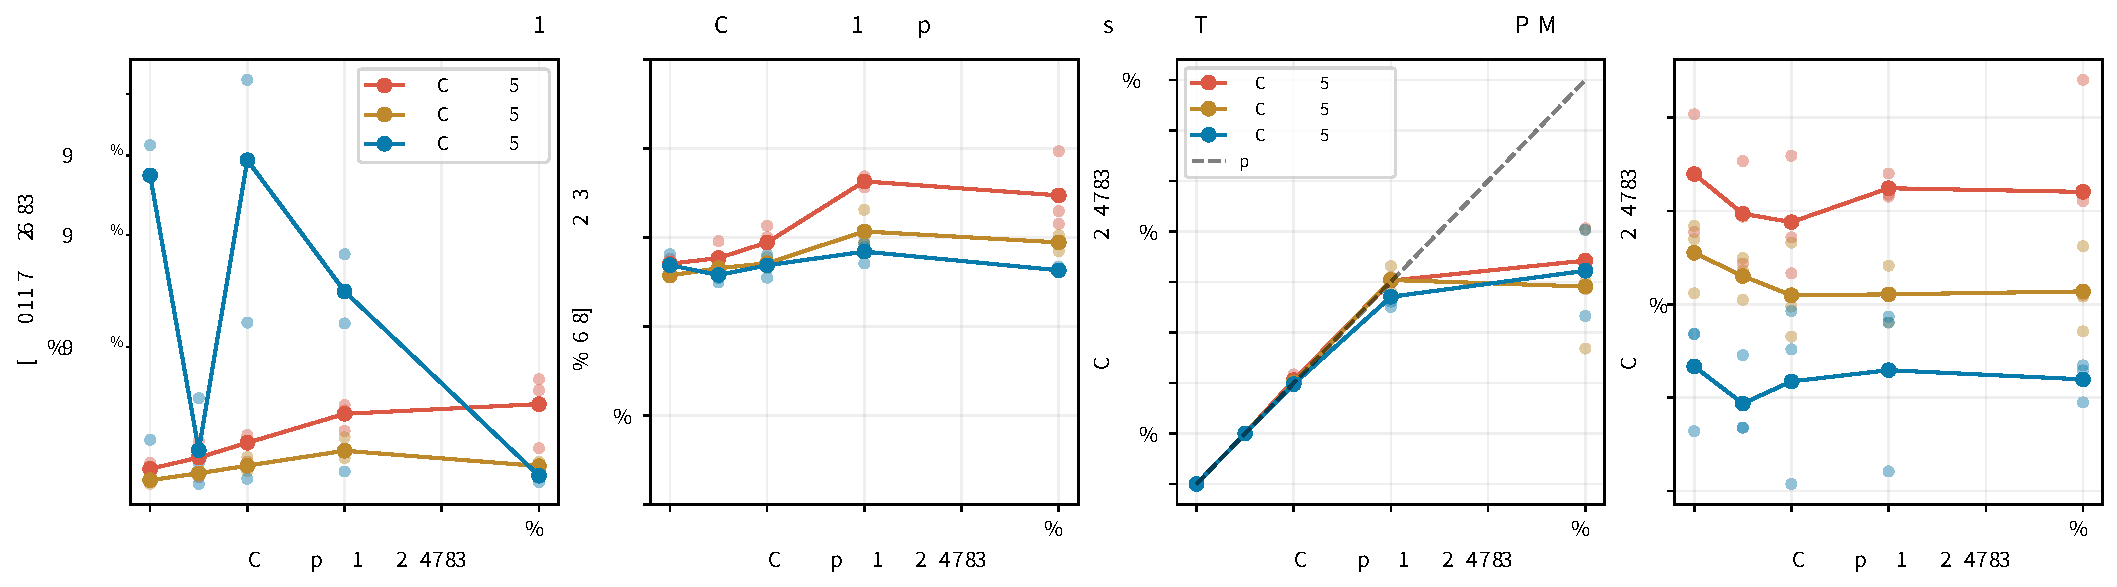
\includegraphics[width=\linewidth]{../experiments/figures/operational/rate-limit-metrics.pdf}\caption{流量制限の通信性能。小さい点は各反復、大きい点は統合値。}\end{figure}
\begin{figure}[htbp]\centering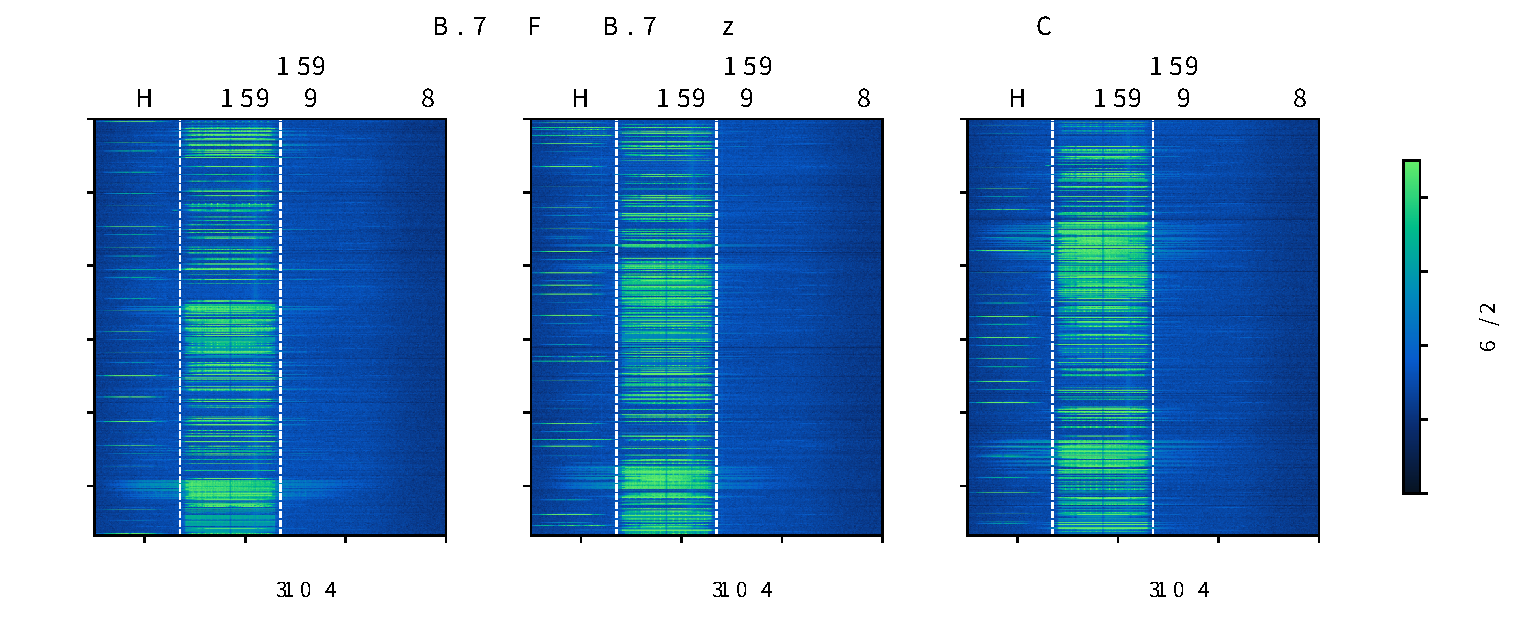
\includegraphics[width=\linewidth]{../experiments/figures/operational/rate-limit-blue-green.pdf}\caption{他チーム通信中の流量比較。共通ゲイン・未校正dBFS。}\end{figure}
\section{生成周期の比較}

流量比較とは別に、同じversion7・helper version2で36試行・12条件・各3反復を新たに取得した。全108000指令、93361応答、20422 I/Q取得。0.5/1 Mbpsの要求量を固定し、TCP byteの生成周期100/10 msを比較する。

\begin{center}\small\begin{adjustbox}{max width=\linewidth}
\begin{tabular}{lllllll}\toprule
他チームCh & 要求 [Mbps] & 生成周期 [ms] & RTT統合p99 [ms] & 20 ms期限超過 [\%] & 自チーム実受信平均 [Mbps] & 他チーム実受信範囲 [Mbps]\\
\midrule
6 & 0.5 & 100 & 132.15 & 54.71 & 0.500 & 2.023–4.069\\
6 & 0.5 & 10 & 135.86 & 58.50 & 0.500 & 2.391–4.081\\
6 & 1 & 100 & 139.05 & 63.47 & 0.971 & 3.694–4.342\\
6 & 1 & 10 & 134.88 & 59.42 & 0.827 & 2.301–3.804\\
7 & 0.5 & 100 & 126.94 & 51.51 & 0.498 & 2.795–2.884\\
7 & 0.5 & 10 & 126.64 & 52.24 & 0.500 & 1.846–2.949\\
7 & 1 & 100 & 127.71 & 53.88 & 0.996 & 1.598–2.676\\
7 & 1 & 10 & 129.90 & 53.88 & 0.996 & 2.561–3.059\\
11 & 0.5 & 100 & 122.42 & 50.26 & 0.499 & 0.089–0.516\\
11 & 0.5 & 10 & 122.11 & 49.91 & 0.500 & 0.140–0.844\\
11 & 1 & 100 & 123.17 & 51.03 & 0.808 & 0.046–1.208\\
11 & 1 & 10 & 121.86 & 50.37 & 0.943 & 0.084–0.704\\
\bottomrule\end{tabular}\end{adjustbox}\end{center}

\subsection{同じ平均要求量と通信品質}

要求1 Mbps・他チームCh6では、100→10 msへの変更で期限超過63.47→59.42\%、RTT統合p99 139.05→134.88 ms、実受信平均0.971→0.827 Mbpsだった。
要求1 Mbps・他チームCh7では、100→10 msへの変更で期限超過53.88→53.88\%、RTT統合p99 127.71→129.90 ms、実受信平均0.996→0.996 Mbpsだった。
要求1 Mbps・他チームCh11では、100→10 msへの変更で期限超過51.03→50.37\%、RTT統合p99 123.17→121.86 ms、実受信平均0.808→0.943 Mbpsだった。

生成周期を小さくする操作は、同じ平均要求量を小分けにする介入である。ただしTCP・OS・MACはbyteをまとめ直せるため、10 ms化でRFの送信が均等になったとは実証していない。画像フレームを丸ごと送る方式と圧縮ストリームを一定量ずつ出す方式に着目するきっかけになるが、実映像・ROS 2のQoS・CPU負荷が異なるシステムへ今回の絶対値を移さない。

実受信量と他チームの負荷実現度も条件間で異なる。期限超過が低下した条件は平均Mbpsだけでは説明できない通信の時間構造を調べる候補になる一方、3反復の変動と反対の変化を示す条件も残して比較する。チャネル、流量、生成周期を一つの介入にまとめず、ロボコンの指令期限に対して個別に検証する。

周期比較の青・緑の図は要求0.5 Mbpsの反復1を全チャネル・両周期で事前指定し、共通ゲインと色尺度で並べる。色の密度から送信周期の実現度や通信成功率を計算しない。


\begin{figure}[htbp]\centering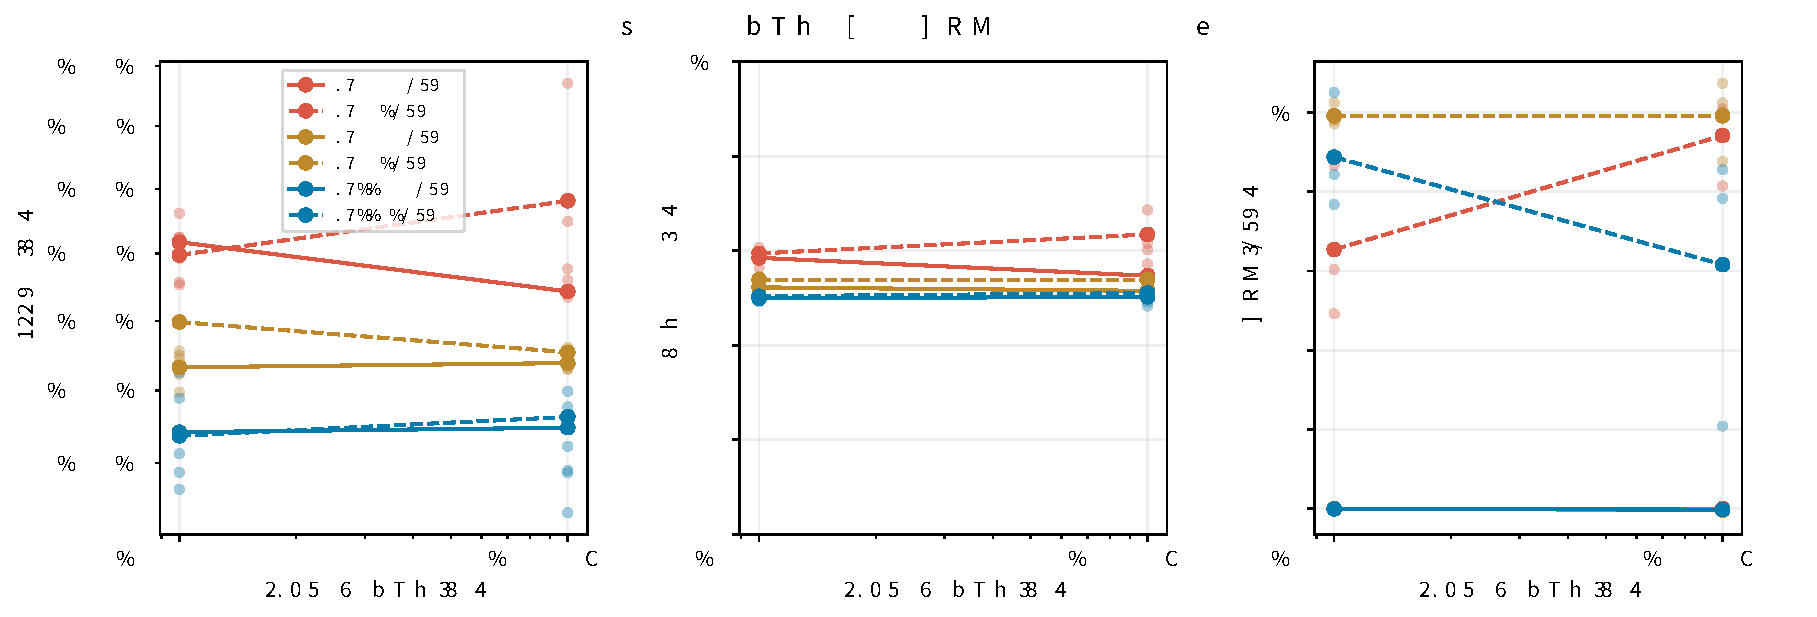
\includegraphics[width=\linewidth]{../experiments/figures/operational/payload-shaping-metrics.pdf}\caption{同じ平均要求量で生成周期を変更した比較。}\end{figure}
\begin{figure}[htbp]\centering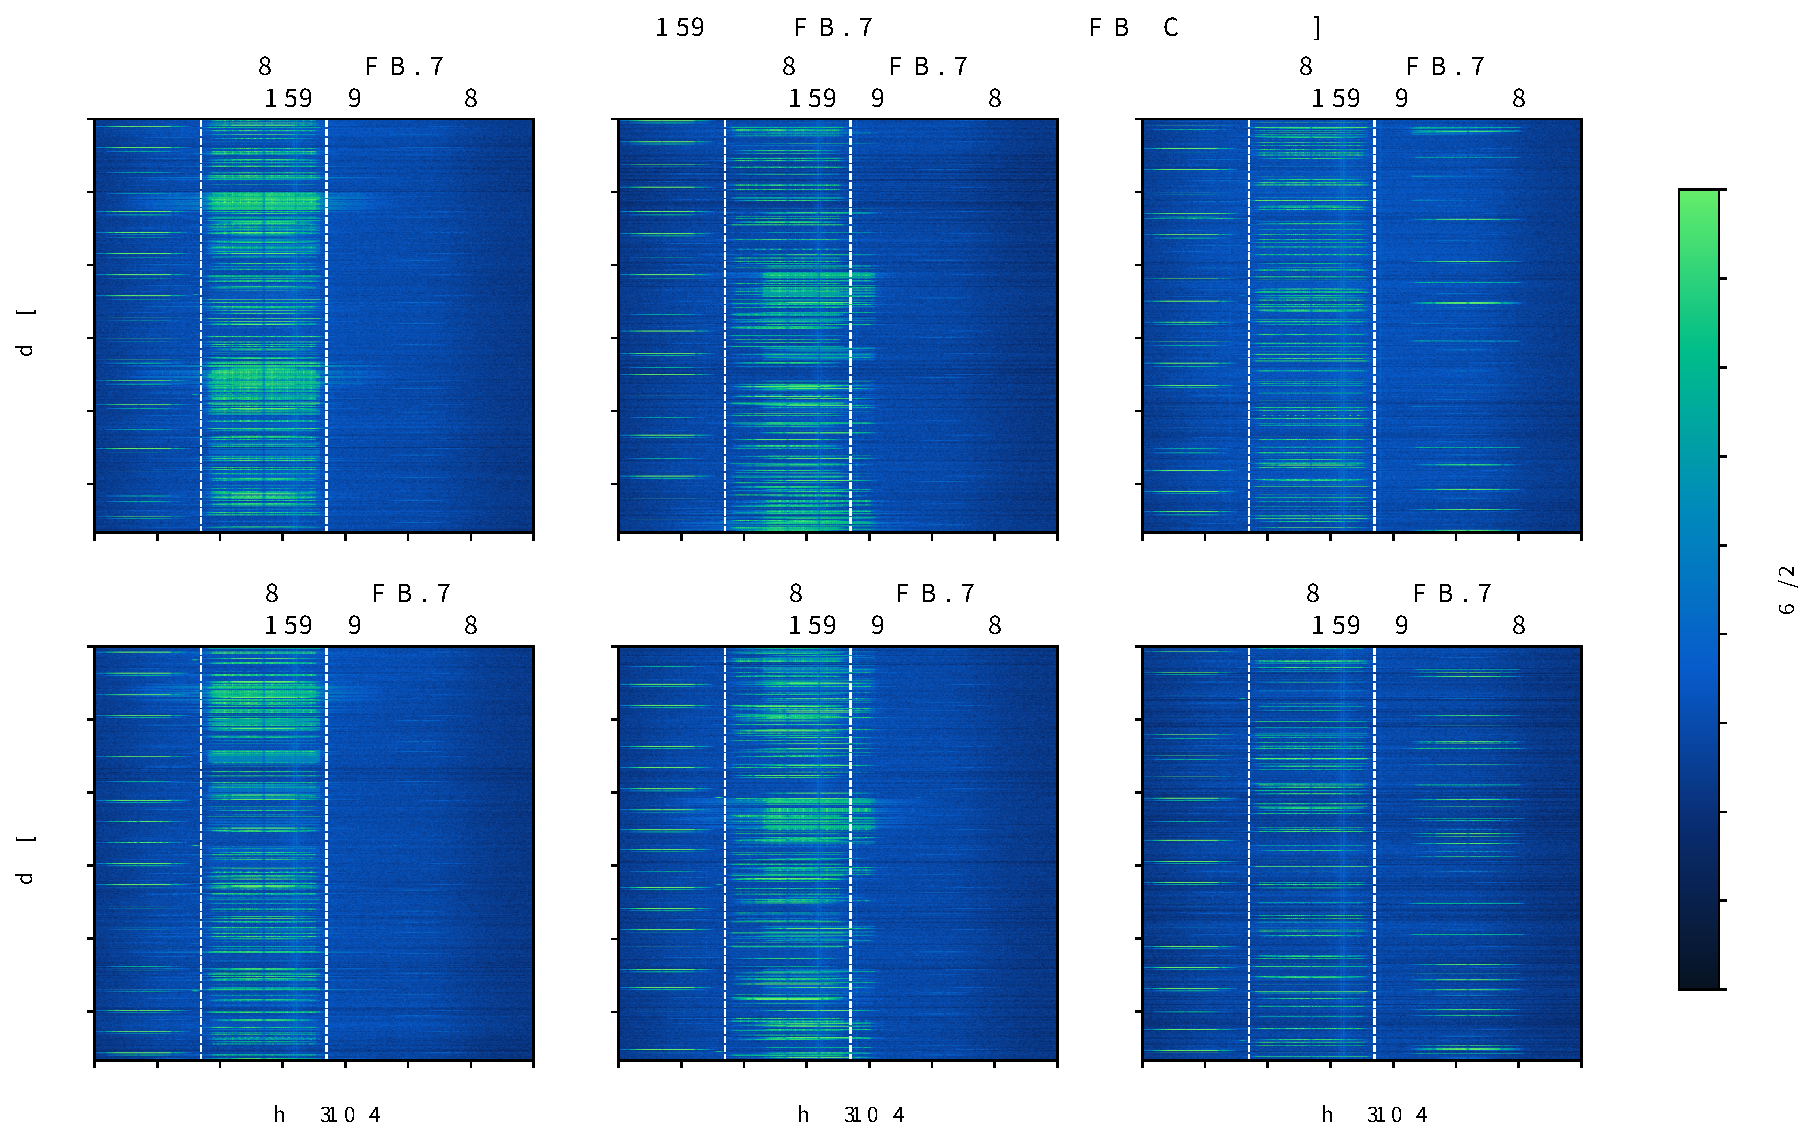
\includegraphics[width=\linewidth]{../experiments/figures/operational/payload-shaping-blue-green.pdf}\caption{生成周期比較の青緑SDR画像。縦軸は間欠取得順。}\end{figure}
\section{実ROS 2のQoSと指令応答}

45試行・15条件・各30秒・3反復。指令側ROS 2 Humble・ロボット側Jazzy、双方CycloneDDS。予定135000指令を全てpublishし、115184 unique応答と25569 I/Q取得を保存した。指令のQoSはreliable・深さ10に固定し、Image／PointCloud2のQoSだけを変更した。PC AP→ロボットSTAの経路であり、前段のSTA→AP→STAとは比較経路が異なる。

\begin{center}\small\begin{adjustbox}{max width=\linewidth}
\begin{tabular}{llllllll}\toprule
センサ負荷 & センサQoS & 深さ & 他チームCh & RTT統合p99 [ms] & 予定指令の20 ms期限超過 [\%] & センサ実受信範囲 [Mbps] & 最長画像更新途絶の反復範囲 [ms]\\
\midrule
heavy & best\_effort & 1 & 6 & 145.57 & 77.68 & 47.83–50.45 & 201.27–205.91\\
heavy & best\_effort & 1 & 7 & 145.54 & 75.92 & 49.84–50.45 & 204.06–226.02\\
heavy & best\_effort & 1 & 11 & 172.27 & 71.54 & 49.05–54.89 & 197.81–3277.47\\
heavy & best\_effort & 10 & 6 & 148.12 & 79.87 & 47.62–48.63 & 197.66–216.89\\
heavy & best\_effort & 10 & 7 & 299.31 & 76.60 & 48.23–50.85 & 205.83–218.86\\
heavy & best\_effort & 10 & 11 & 256.96 & 72.53 & 47.86–55.09 & 191.31–3327.43\\
heavy & reliable & 1 & 6 & 146.44 & 77.92 & 47.42–49.04 & 205.24–218.82\\
heavy & reliable & 1 & 7 & 146.48 & 76.40 & 49.64–51.05 & 204.77–232.86\\
heavy & reliable & 1 & 11 & 135.64 & 70.46 & 52.08–55.09 & 192.55–601.71\\
heavy & reliable & 10 & 6 & 155.70 & 79.57 & 47.02–48.82 & 206.12–208.56\\
heavy & reliable & 10 & 7 & 149.15 & 76.98 & 48.63–50.85 & 204.42–217.73\\
heavy & reliable & 10 & 11 & 136.11 & 70.43 & 54.67–54.89 & 197.24–375.54\\
off & best\_effort & 1 & 6 & 104.10 & 46.06 & 0.00–0.00 & —\\
off & best\_effort & 1 & 7 & 111.84 & 45.12 & 0.00–0.00 & —\\
off & best\_effort & 1 & 11 & 109.91 & 44.56 & 0.00–0.00 & —\\
\bottomrule\end{tabular}\end{adjustbox}\end{center}

指令のみの条件にも約100 ms級のRTT p99と約45\%の20 ms期限超過がある。センサを止めても指令期限を満たしていないため、カメラ帯域を削減するだけで解決すると結論できない。センサを加えると期限超過はおよそ70〜80\%となり、同じWi-Fiに大容量トピックを載せた状態で指令品質を検証する必要がある。

best effort・深さ1を常に最善とする結果でも、reliableの優位を一般化する結果でもない。同じQoSでも反復ごとの尾部遅延と更新途絶が変わる。深さ1はアプリの受信履歴設定であり、無線の待ち行列を深さ1にする操作ではない。センサの受信更新間隔を指令RTTと併記することで、操縦指令の遅れとカメラ・点群の更新停止を分けて評価できる。センサの更新間隔は各sequenceの初回受信の間隔であり、古いsequenceの遅着を除くESP-NOWの最新sequence更新間隔とは異なる。異なるPCの時計は引いておらず、センサの生成から到着までの絶対的な古さは測っていない。

センサの要求data payloadは60.53888 Mbpsだが、実受信はおよそ47〜55 Mbpsである。publishが遅れた古い生成slotは飛ばしているため、未生成・publish済み・測定窓内受信を分ける。センサ内容は合成データであり、圧縮映像、実LiDARの処理負荷やモータ制御を再現していない。

他チームの飽和TCPは全試行で現行相手のnonce/challengeと実受信増加を確認したが、チャネルごとの実受信量は揃っていない。Ch11の20 MHz信号の一部はC5の48 MHzアナログ帯域の名目端の外へかかるため、青緑SDR図の弱い色から干渉がなくなったとは言えない。

認証による転送停止前の28試行と、回収・再開後の17試行をそのまま保持した。取得セグメント、転送方法、転送元SHA256を記録し、性能を理由に悪い試行を再測定していない。再開前後の時間帯・環境変動は統制できていない。

ロボコンでの実装候補は、指令と大容量トピックの用途別QoS、画像・点群の生成量や周期、省電力設定を個別に変え、予定指令の期限超過と最新データの途絶を測ることである。QoS設定だけで通信の優先度や20 ms期限が保証される結果にはなっていない。


\begin{figure}[htbp]\centering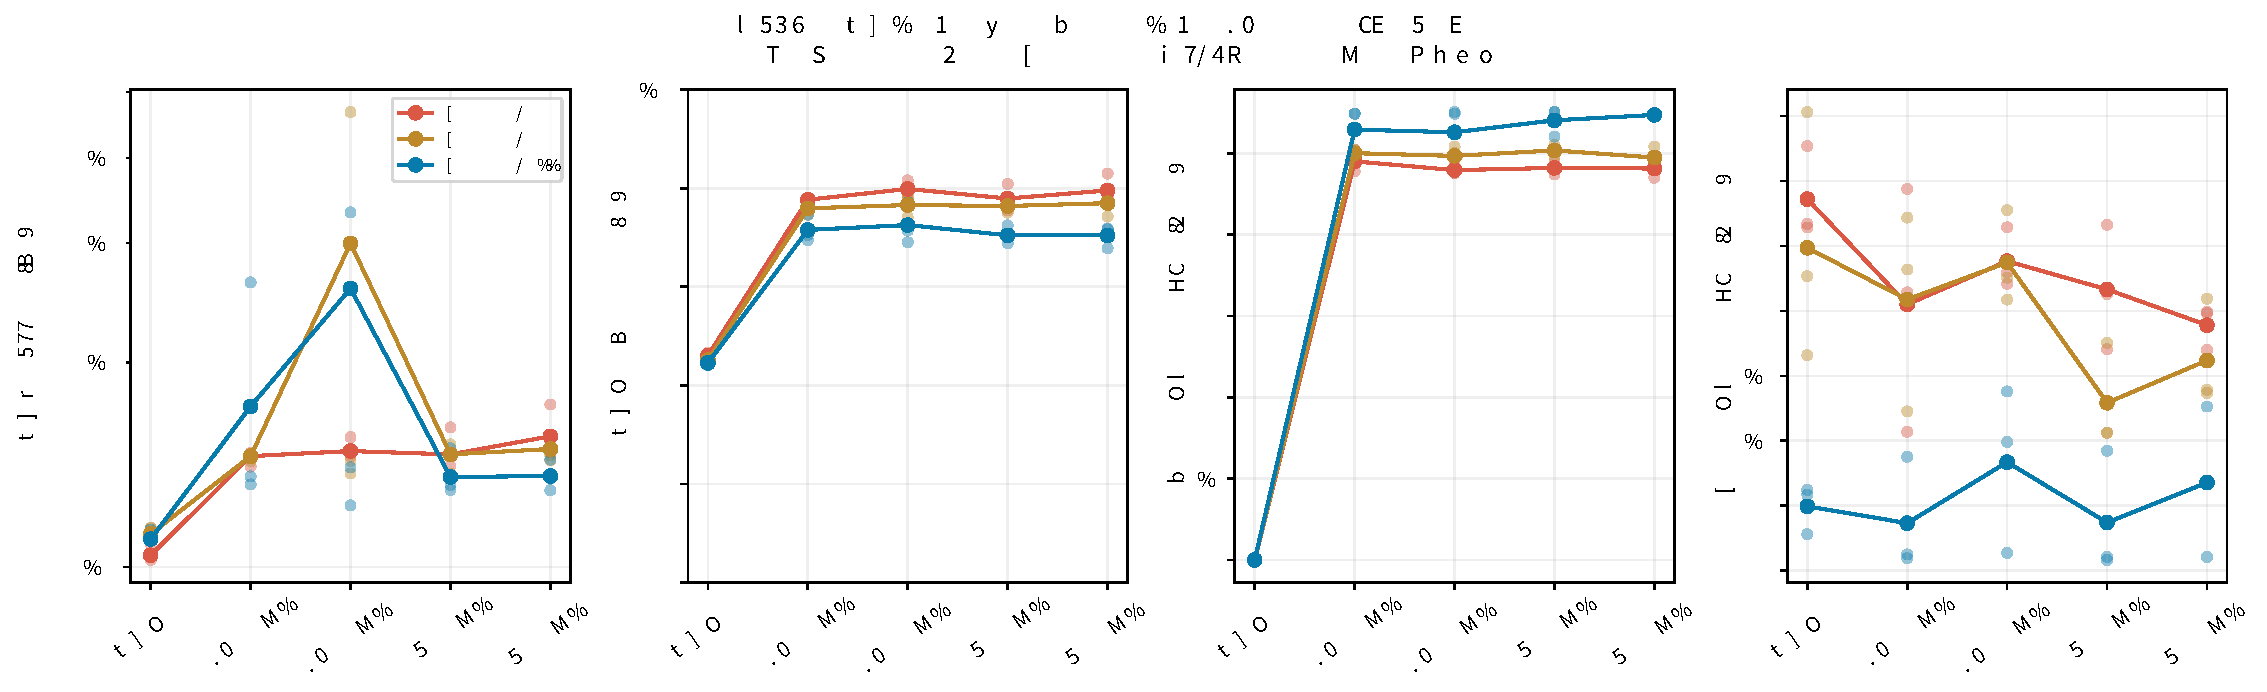
\includegraphics[width=\linewidth]{../experiments/figures/operational/ros2-qos-metrics.pdf}\caption{実ROS 2のQoS比較。センサQoSのみ変更し、指令QoSは固定。}\end{figure}
\begin{figure}[htbp]\centering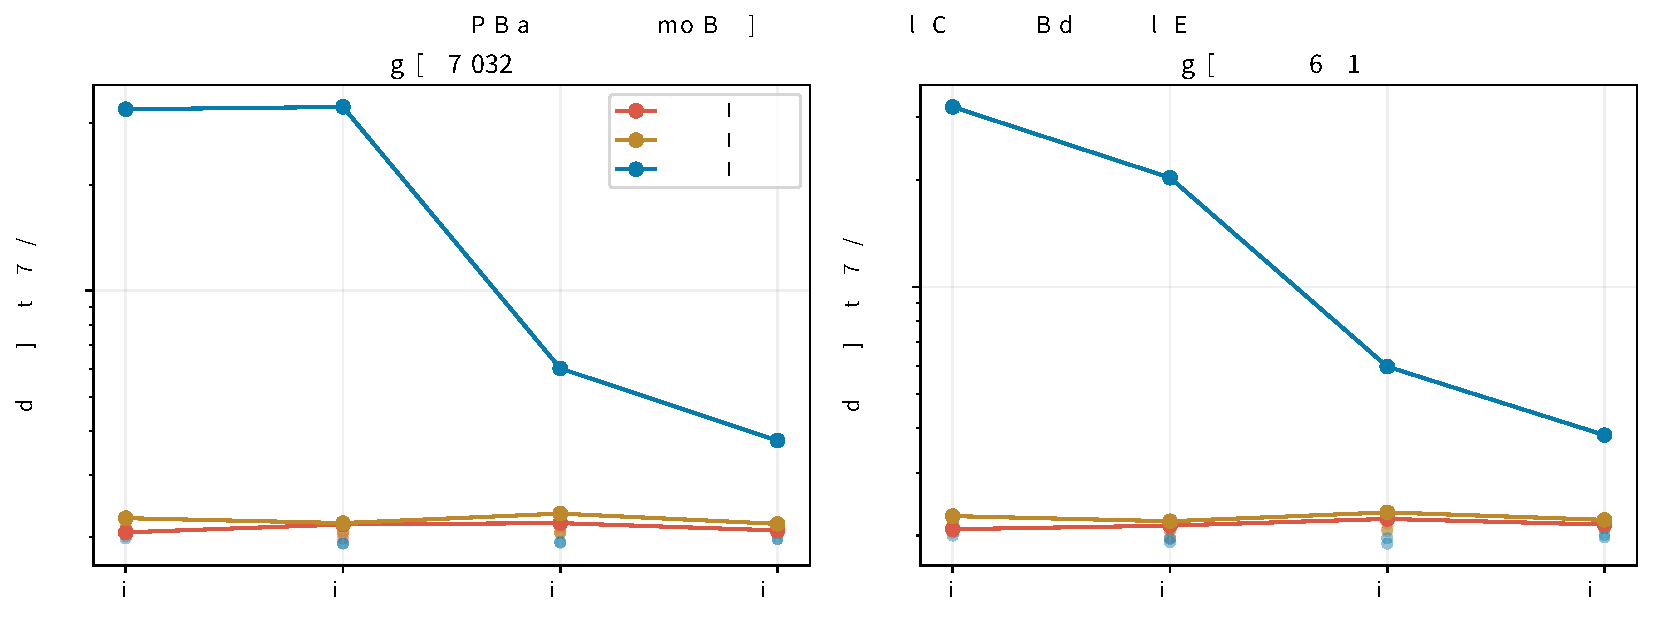
\includegraphics[width=\linewidth]{../experiments/figures/operational/ros2-update-gaps.pdf}\caption{画像と点群の各unique sequence初回受信の更新間隔。}\end{figure}
\begin{figure}[htbp]\centering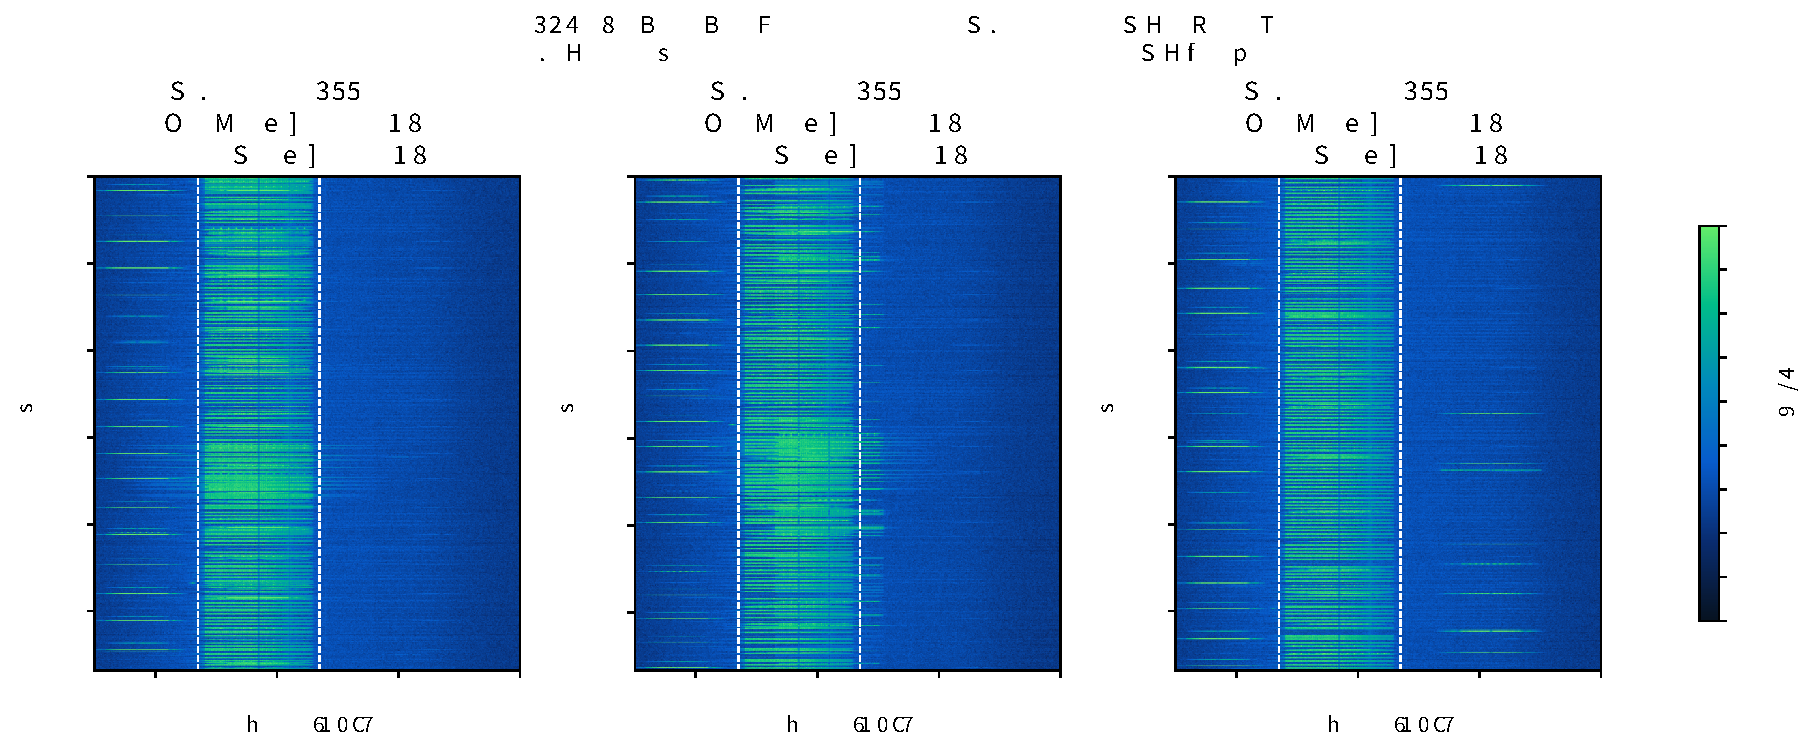
\includegraphics[width=\linewidth]{../experiments/figures/operational/ros2-blue-green.pdf}\caption{実ROS 2通信と別チーム負荷。色から配送成功や占有率は計算できない。}\end{figure}
\section{省電力設定への介入と端末内時間}

QoS比較とは別に24試行・8条件・各30秒・3反復。予定72000指令、publish済み72000指令、63334 unique応答、13650 I/Q取得。STAの省電力ON／OFFを実際に切り替え、各試行の前後にiwのreadbackを保存した。AP側はOFFに固定した。センサQoSはbest effort・深さ1、指令はreliable・深さ10。

\begin{center}\small\begin{adjustbox}{max width=\linewidth}
\begin{tabular}{llllllll}\toprule
センサ負荷 & 他チームCh & STA省電力 & RTT統合p99 [ms] & 20 ms期限超過 [\%] & 予定送信のずれ統合p99 [ms] & 指令publish統合p99 [ms] & callbackから応答publish前までp99の範囲 [ms]\\
\midrule
off & 6 & off & 106.29 & 46.23 & 0.995 & 0.077 & 0.0048–0.0061\\
off & 6 & on & 108.53 & 46.76 & 1.003 & 0.082 & 0.0039–0.0051\\
off & 11 & off & 103.61 & 44.48 & 0.513 & 0.085 & 0.0043–0.0054\\
off & 11 & on & 103.27 & 44.41 & 1.022 & 0.081 & 0.0040–0.0071\\
heavy & 6 & off & 157.88 & 79.86 & 1.044 & 0.087 & 0.0031–0.0036\\
heavy & 6 & on & 153.24 & 80.28 & 1.033 & 0.086 & 0.0027–0.0033\\
heavy & 11 & off & 163.38 & 72.54 & 0.998 & 0.086 & 0.0032–0.0034\\
heavy & 11 & on & 248.66 & 75.76 & 1.027 & 0.086 & 0.0026–0.0032\\
\bottomrule\end{tabular}\end{adjustbox}\end{center}

\subsection{同じ負荷条件でのOFFからONへの変化}

センサoff・他チームCh6で省電力OFF→ONにすると、RTT統合p99は106.29→108.53 ms、20 ms期限超過は46.23→46.76\%だった。
センサoff・他チームCh11で省電力OFF→ONにすると、RTT統合p99は103.61→103.27 ms、20 ms期限超過は44.48→44.41\%だった。
センサheavy・他チームCh6で省電力OFF→ONにすると、RTT統合p99は157.88→153.24 ms、20 ms期限超過は79.86→80.28\%だった。
センサheavy・他チームCh11で省電力OFF→ONにすると、RTT統合p99は163.38→248.66 ms、20 ms期限超過は72.54→75.76\%だった。

ON／OFFは設定要求だけでなく取得前後の実readbackで確認した介入である。ただしiwの状態は、実際に何ms眠ったかや無線の待ち時間を直接測った値ではない。他チームの実受信量やセンサ実配送も変動するため、効果を端末一般の保証へ広げない。

予定送信のずれとpublish呼出しはコントローラー内の時計、callbackから応答publish前までの処理はロボット内の時計、往復応答はコントローラーの時計で測った。publishが短くても、その後のDDS・OS・MACの待ち行列、無線再送、受信dispatchの時間は残る。p99同士を引いて各原因の寄与を割り当てたり、RTTの半分を片道遅延と扱ったりしない。

ロボコンで確認すべきなのは、実際の端末で省電力設定を変えたときに、指令の期限超過と最長更新途絶がどう変わるかである。省電力OFF・チャネル分離・QoS設定を組み合わせても、今回の試験で満たしていない期限を満たしたものとして扱わない。測定中に監視用HTTPを周期送信せず、終了後にログを転送した。


\begin{figure}[htbp]\centering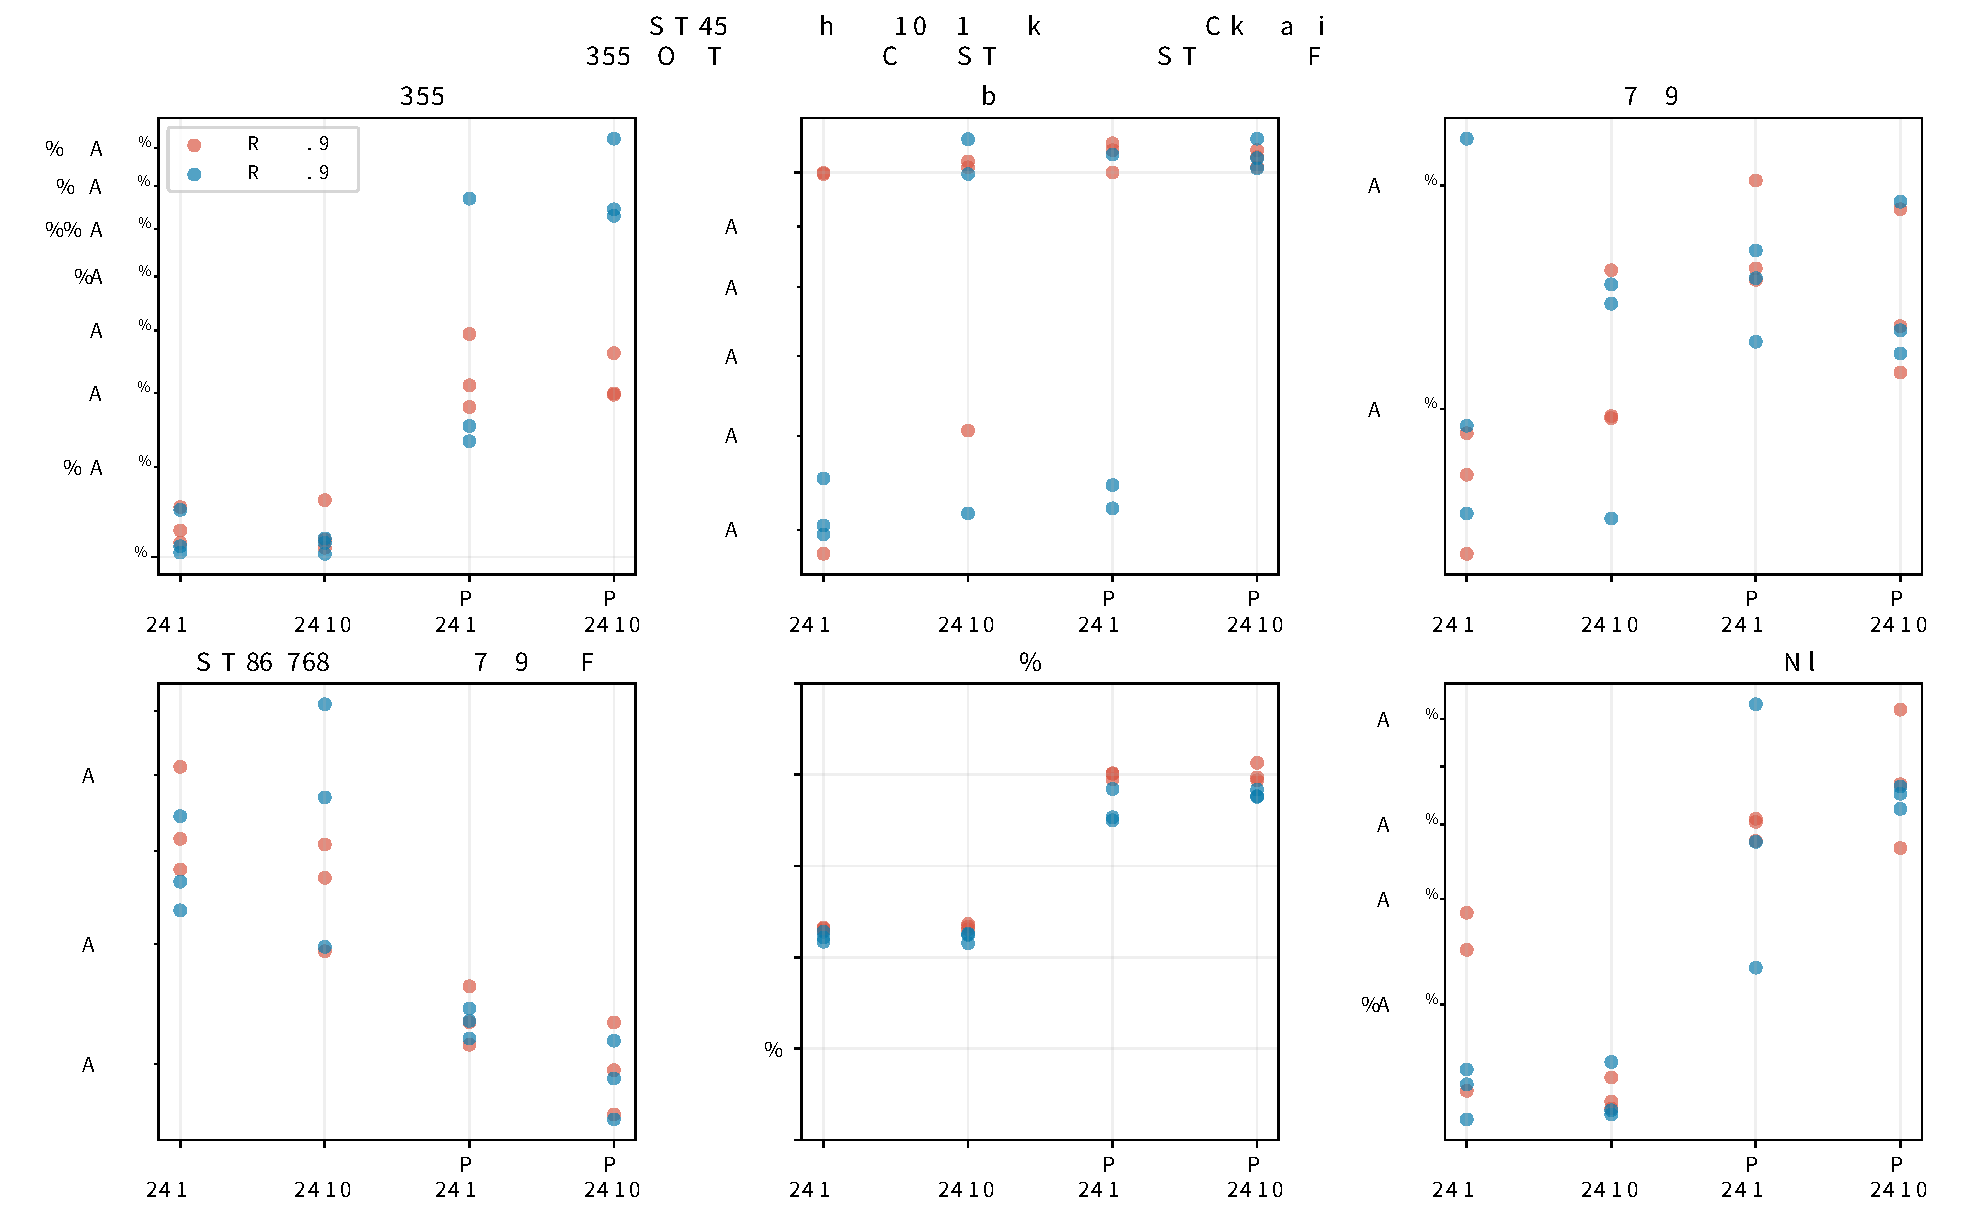
\includegraphics[width=\linewidth]{../experiments/figures/operational/power-save-timing.pdf}\caption{省電力ON/OFFと同じ端末時計内の処理時間。}\end{figure}
\begin{figure}[htbp]\centering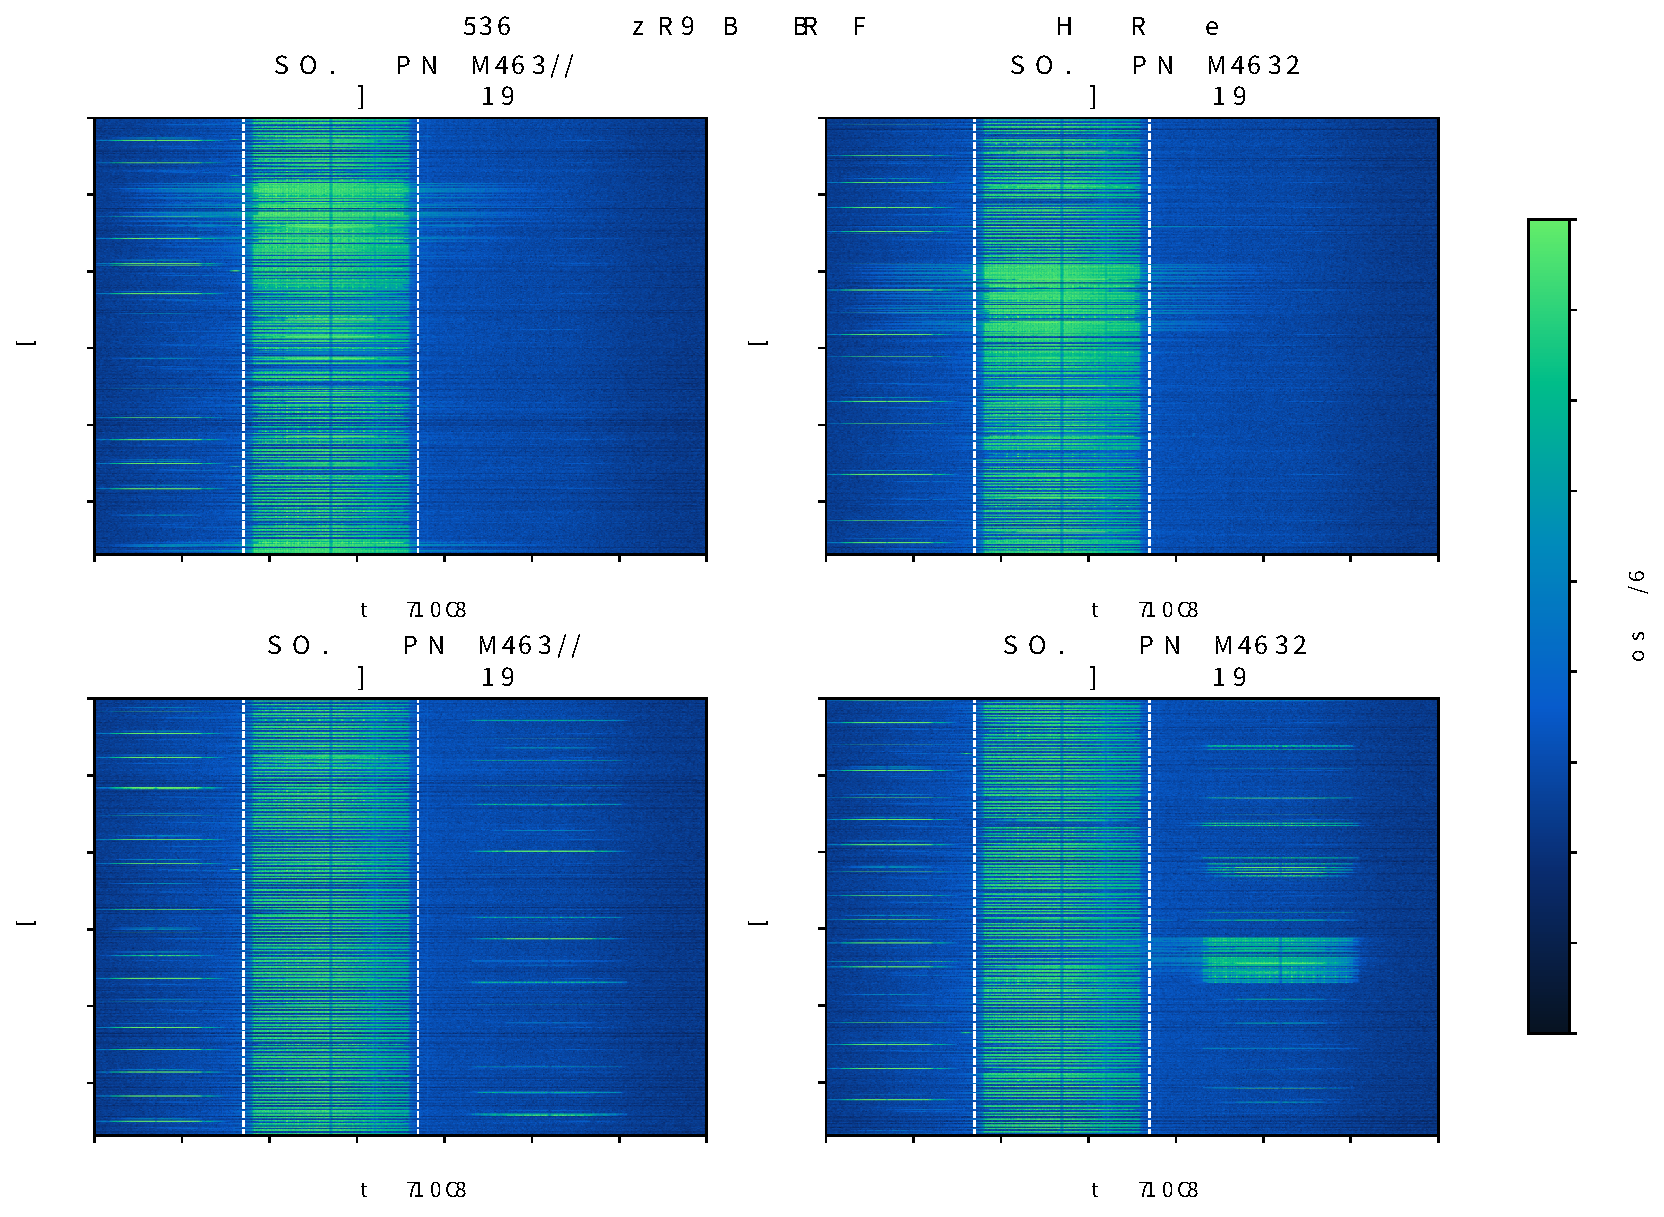
\includegraphics[width=\linewidth]{../experiments/figures/operational/power-save-blue-green.pdf}\caption{省電力比較の実測SDR画像。}\end{figure}
\section{ESP-NOWの指令周期と長時間更新の安定性}

当初24試行の予定だったが、使用者が実験を早く終えたいと希望したため、進行中の試行を保存した19試行で長時間測定を終了した。残り5試行は測っていない。反復1・2は全8条件、反復3は3条件である。取得した全試行を残し、条件間の反復数が異なることを明記する。

19試行・8条件・各600秒・条件ごと2〜3反復。予定960000指令、960000送信呼出し、959997 unique応答、215489 I/Q取得を保存した。ESP32 2台間の64 byteアプリ応答を20・50・100・200 Hzで連続記録し、別系統のCh6・20 MHz Wi-Fiを待機／TCP負荷に切り替えた。配置は同じ机上のおおむね30 cmという使用者の申告であり、正確な送受信距離は未測定。

\begin{center}\small\begin{adjustbox}{max width=\linewidth}
\begin{tabular}{llllllll}\toprule
指令周期 [Hz] & Wi-Fi & 反復数 & RTT統合p99 [ms] & 予定指令の20 ms期限超過 [\%] & 応答欠落 / 予定指令 & 新しいsequenceへの最長更新途絶の反復範囲 [ms] & Wi-Fi実受信範囲 [Mbps]\\
\midrule
20 & heavy & 2 & 9.179 & 0.01667 & 2 / 24000 & 100.260–100.737 & 2.375–2.531\\
20 & off & 3 & 9.229 & 0.01944 & 1 / 36000 & 61.126–99.992 & 0.000–0.000\\
50 & heavy & 3 & 9.616 & 0.02667 & 0 / 90000 & 37.717–46.460 & 1.728–2.723\\
50 & off & 3 & 8.922 & 0.00667 & 0 / 90000 & 32.591–47.182 & 0.000–0.000\\
100 & heavy & 2 & 9.264 & 0.00083 & 0 / 120000 & 23.644–23.854 & 2.223–2.598\\
100 & off & 2 & 10.711 & 0.03500 & 0 / 120000 & 23.021–49.788 & 0.000–0.000\\
200 & heavy & 2 & 14.262 & 0.21083 & 0 / 240000 & 35.341–36.799 & 1.920–2.080\\
200 & off & 2 & 12.746 & 0.13458 & 0 / 240000 & 18.638–32.496 & 0.000–0.000\\
\bottomrule\end{tabular}\end{adjustbox}\end{center}

\subsection{Wi-Fi待機と負荷の比較}

20 HzでWi-Fi待機→負荷へ切り替えたとき、RTT統合p99は9.229→9.179 ms、予定指令の20 ms期限超過は0.01944→0.01667\%、応答欠落は1→2件だった。
50 HzでWi-Fi待機→負荷へ切り替えたとき、RTT統合p99は8.922→9.616 ms、予定指令の20 ms期限超過は0.00667→0.02667\%、応答欠落は0→0件だった。
100 HzでWi-Fi待機→負荷へ切り替えたとき、RTT統合p99は10.711→9.264 ms、予定指令の20 ms期限超過は0.03500→0.00083\%、応答欠落は0→0件だった。
200 HzでWi-Fi待機→負荷へ切り替えたとき、RTT統合p99は12.746→14.262 ms、予定指令の20 ms期限超過は0.13458→0.21083\%、応答欠落は0→0件だった。

\subsection{応答欠落を記録した試行}

20 Hz・Wi-Fi heavy・反復1：予定12000、送信呼出し12000、unique応答11999。応答機の受信カウンタ12000、応答送信APIエラー0、MAC送信失敗1、echo queue drop0。指令機のMAC送信失敗0、UART trace drop0。
20 Hz・Wi-Fi heavy・反復2：予定12000、送信呼出し12000、unique応答11999。応答機の受信カウンタ12000、応答送信APIエラー0、MAC送信失敗1、echo queue drop0。指令機のMAC送信失敗0、UART trace drop0。
20 Hz・Wi-Fi off・反復2：予定12000、送信呼出し12000、unique応答11999。応答機の受信カウンタ12000、応答送信APIエラー0、MAC送信失敗1、echo queue drop0。指令機のMAC送信失敗0、UART trace drop0。

これらは試行全体のカウンタであり、MAC結果を個々の欠落sequenceへ対応づけていない。Wi-Fi待機条件でも欠落がある場合、全欠落を追加TCP負荷の影響として扱わない。

\subsection{指令の往復時間と情報の更新間隔}

20 Hzの通常更新間隔は50 ms、200 Hzは5 msである。20 ms期限超過は各指令の予定送信から応答までを測る比較指標であり、20 Hzの制御情報が20 msごとに更新されるという意味ではない。最長更新途絶には通常の指令周期も含むため、周期の違う条件を欠落率だけ、あるいは途絶の絶対値だけで順位付けしない。新しいsequenceが届いた時刻で途絶を計算し、古い応答の到着を新しい制御情報の更新に数えない。

64 byteの要求を100 Hzで送るアプリpayloadは片方向0.0512 Mbps、200 Hzでは0.1024 Mbpsであり、全要求に同サイズの応答がある場合は往復合計がその2倍になる。これはフレームヘッダー、プリアンブル、ACK、送信待ち、再送を含む空中時間ではない。設定PHY 1 Mbpsも受信アナログ帯域やアプリ実到達量ではない。小さな指令を高頻度で送る設計では、平均payloadだけでなく周期と更新途絶を検証する。

送信API受付、MAC送信結果、相手からのアプリ応答は別々の観測である。MAC成功は相手アプリの実行やロボットの動作を保証しない。この区別は\href{https://docs.espressif.com/projects/esp-idf/en/v6.0/esp32/api-reference/network/esp\_now.html\#send-esp-now-data}{EspressifのESP-NOWガイド}でも示されている。応答がない場合も、往路の指令が届かなかったのか復路の応答が欠けたのかを送信側の記録だけで決められない。連続記録のCRC、予定slot、END、UART dropを検算し、テレメトリ欠落を無線欠落として数えない。

\subsection{Wi-Fiとの共存と適用範囲}

Wi-Fi TCPの要求payloadは15.72864 Mbpsであり、達成量は表の実受信値である。要求が同じでも実受信と空中時間は同じとは限らない。待機にもAPビーコンと監視通信があり、電波が完全に停止した基準ではない。10秒ごとのカウンタで接続と実通信を確認するが、瞬間ごとのRF送信量は測っていない。

ESP-NOWは今回の設定ではルーターを通らない独立リンクである。ROS 2のPC間通信やSTA→AP→STAのUDPと経路、端末、実装、配置が異なるため、絶対RTTの差をプロトコル固有の優劣として扱わない。ロボコンへの示唆は、大容量データと指令の経路を分ける候補でも、同じチャネルで両者を実際に動かして更新途絶を測る必要があることにある。連続10分を3回測っても、会場、遮蔽、移動、長距離や安全停止の保証にはならない。欠落ゼロの条件も、将来の欠落確率ゼロを意味しない。

C5のRF記録は連続ではなく間欠取得であり、アプリイベントの全時間軸とは別である。青緑の色は未校正dBFSを共通尺度で表示した受信エネルギーで、ESP-NOWの成功率、Wi-Fi占有率、送信電力ではない。

\section{ESP32間通信の配置・向き・遮蔽比較}

使用者が適用・確認した5配置、Wi-Fi待機／負荷、各10秒・3反復の30試行。予定30000指令、30000送信呼出し、30000 unique応答、5641 I/Q取得。ESP32 2台間のESP-NOW Ch6・100 Hzを評価対象とし、PC間の距離は比較指標にしていない。距離はボードまたはケース中心間の使用者報告値で、アンテナ間距離の校正値ではない。

\begin{center}\small\begin{adjustbox}{max width=\linewidth}
\begin{tabular}{llllll}\toprule
配置 & ESP32送受信間 [cm] & C5と指令機 [cm] & C5と応答機 [cm] & 応答機の回転 [°] & 遮蔽物\\
\midrule
基準・前 & 75 & 45 & 95 & 0 & なし\\
90°回転 & 75 & 45 & 95 & 90 & なし\\
遮蔽 & 75 & 45 & 95 & 0 & 手\\
距離変更 & 150 & 45 & 157 & 0 & なし\\
基準・後 & 75 & 45 & 95 & 0 & なし\\
\bottomrule\end{tabular}\end{adjustbox}\end{center}

90°回転の距離注記：回転後の中心間距離は基準とほぼ同じとの申告。基準の75/45/95 cmを使用し、回転後に厳密に再測定した値ではない。

遮蔽の距離注記：基板は基準位置のまま、基準の申告距離75/45/95 cmを使用。遮蔽時に厳密に再測定した値ではない。

距離変更の距離注記：送受信150 cm、C5→M5 157 cmは移動後の使用者報告。固定C5→送信45 cmは基準値を使用。

基準・後の距離注記：最初の位置・向きへ戻したとの申告。基準の75/45/95 cmを使用し、復帰後に厳密に再測定した値ではない。

\begin{center}\small\begin{adjustbox}{max width=\linewidth}
\begin{tabular}{llllllll}\toprule
配置 & Wi-Fi & RTT統合p99 [ms] & 20 ms期限超過 [\%] & 応答欠落 / 予定指令 & 最長更新途絶 [ms] & 応答機の最新RSSIの反復範囲 [dBm] & Wi-Fi実受信範囲 [Mbps]\\
\midrule
基準・前 & off & 11.185 & 0.033 & 0 / 3000 & 24.994 & -43–-40 & 0.000–0.000\\
基準・前 & heavy & 10.908 & 0.000 & 0 / 3000 & 24.320 & -46–-42 & 1.095–1.549\\
90°回転 & off & 8.381 & 0.000 & 0 / 3000 & 20.563 & -45–-38 & 0.000–0.000\\
90°回転 & heavy & 7.789 & 0.000 & 0 / 3000 & 16.918 & -45–-42 & 1.108–1.499\\
遮蔽 & off & 8.254 & 0.000 & 0 / 3000 & 19.712 & -37–-36 & 0.000–0.000\\
遮蔽 & heavy & 7.933 & 0.000 & 0 / 3000 & 20.161 & -37–-36 & 1.355–1.484\\
距離変更 & off & 8.508 & 0.000 & 0 / 3000 & 22.747 & -43–-40 & 0.000–0.000\\
距離変更 & heavy & 8.832 & 0.000 & 0 / 3000 & 20.385 & -41–-40 & 1.310–1.472\\
基準・後 & off & 8.415 & 0.000 & 0 / 3000 & 17.988 & -31–-30 & 0.000–0.000\\
基準・後 & heavy & 8.630 & 0.000 & 0 / 3000 & 19.250 & -31–-30 & 1.092–1.356\\
\bottomrule\end{tabular}\end{adjustbox}\end{center}

\subsection{基準配置の前後と条件比較}

Wi-Fi offの基準・前→基準・後では、RTT統合p99が11.185→8.415 ms、20 ms期限超過が0.033→0.000\%だった。
Wi-Fi heavyの基準・前→基準・後では、RTT統合p99が10.908→8.630 ms、20 ms期限超過が0.000→0.000\%だった。
Wi-Fi負荷中の90°回転では、基準・前から20 ms期限超過が0.000→0.000\%、応答欠落が0→0件に変わった。
Wi-Fi負荷中の遮蔽では、基準・前から20 ms期限超過が0.000→0.000\%、応答欠落が0→0件に変わった。
Wi-Fi負荷中の距離変更では、基準・前から20 ms期限超過が0.000→0.000\%、応答欠落が0→0件に変わった。

今回の全配置で予定指令に対する応答欠落はなかった。ただし期限超過は応答欠落と別であり、届いた全指令が20 ms以内だったという意味ではない。この近距離・短時間試験では、向き・手・距離変更による応答不達の増加を捉えなかった。リンクの受信余裕が大きい場合、姿勢や反射が変わっても配送が保たれ得る。遠距離や金属筐体の遮蔽で同じ余裕があるかは今回の配置から判断できない。

負荷中の基準・後も基準・前よりRTT p99が低かった。したがって変更条件のp99低下を、回転や遮蔽だけの改善効果と結論できない。元に戻した条件にも変化が残ることが、時間経過・端末状態・ケーブルや室内反射を比較に含める必要性を示す。ロボットのアンテナ配置を決める際も、基準へ戻す測定を挟む価値がある。

各配置をまとめて測るため、配置間の順序は無作為化していない。基準・前後の変動と各反復を併せて示し、一つの良い／悪い試行だけで配置を順位付けしない。Wi-Fi実受信量も比較に併記し、負荷実現度の変化を配置の効果だけへ帰属しない。

\subsection{RSSI・SDR画像と指令品質の関係}

表のRSSIは各反復の終了時に読み出した最後の受信パケットの値である。3点の最小・最大は全パケットの分布や試行平均ではない。新しい受信のない試行には以前のRSSIを流用しない。RSSIが改善しても期限超過が減るとは限らず、欠落時の信号強度は観測できない。

手または身体を2台の間へ置いた操作を評価したもので、人体・ロボット筐体の一般的な遮蔽損失を測った校正実験ではない。応答機の回転にはケーブルと周囲の反射の変化も伴い得る。距離点が少なく、近い机上配置なので到達距離や自由空間伝搬の式を推定しない。

C5の青緑画像は各配置のWi-Fi負荷・反復1を事前指定して共通設定と色尺度で並べる。応答機を移動するとC5までの距離も変わるため、画像の色は通信相手のRSSIと同じ量ではない。10秒窓で色の違いが見えなくても、人体や向きが影響しないと一般化しない。

ロボコンでは、実機搭載位置、コントローラーの向き、人や金属物の位置を変え、大容量通信中に指令がいつまで更新されないかを測る比較へ展開できる。今回の各10秒・3反復を会場全体の性能保証や600秒試行と同じ耐久性へ読み替えない。
\begin{figure}[htbp]\centering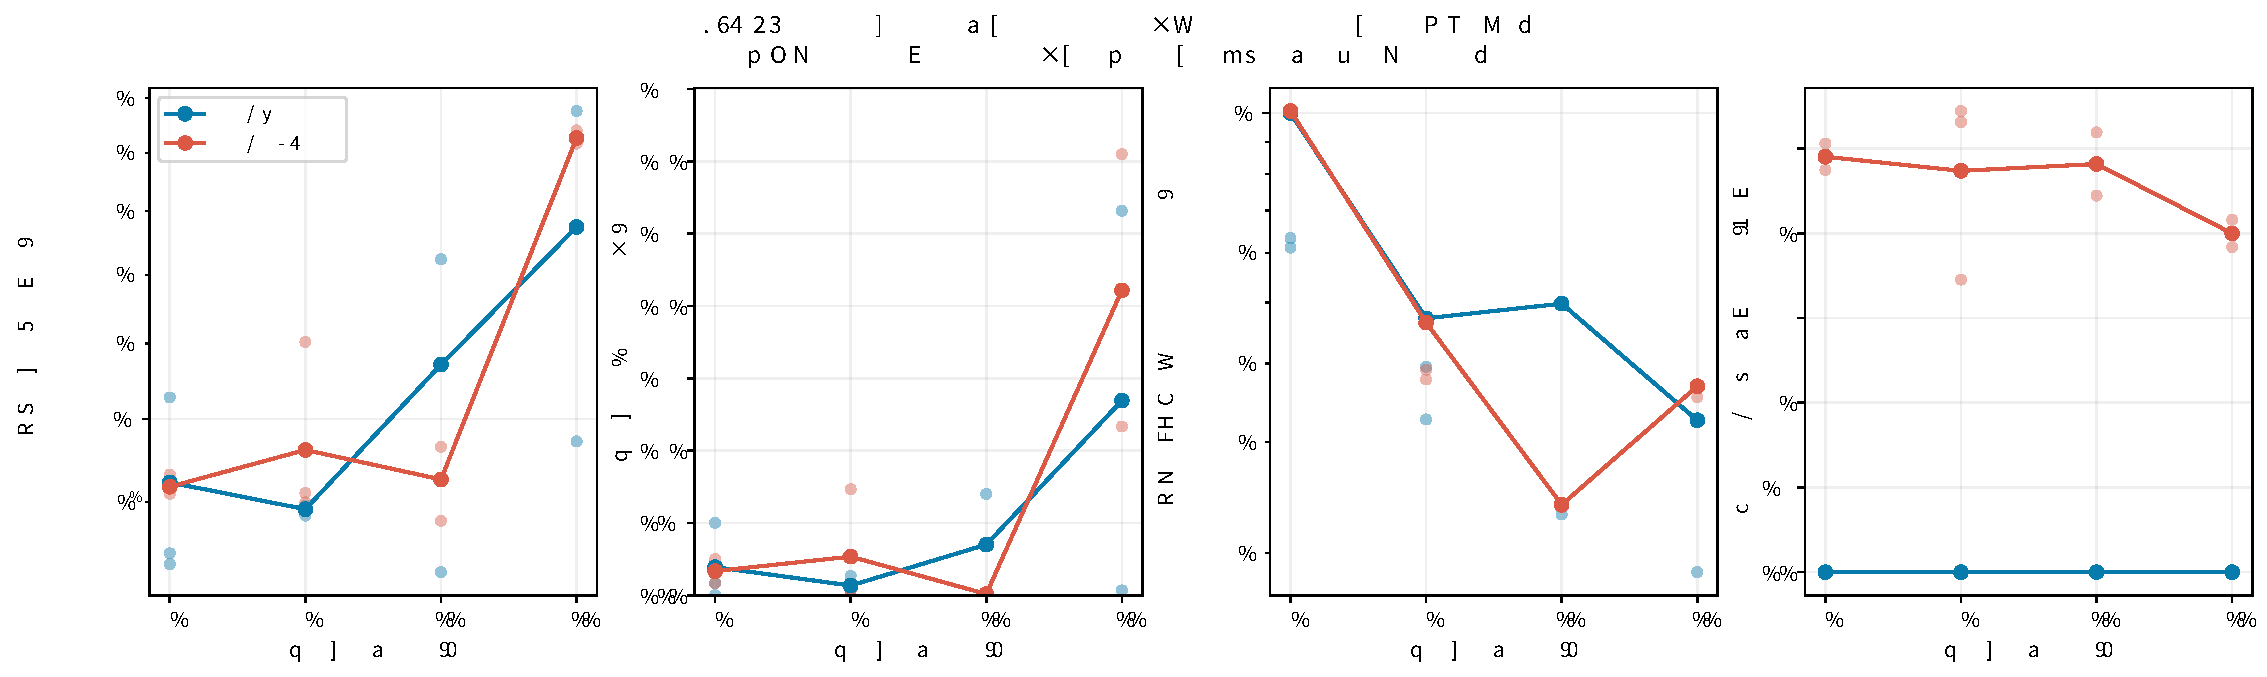
\includegraphics[width=\linewidth]{../experiments/figures/operational/espnow-long-metrics.pdf}\caption{600秒ESP-NOW試行。19試行、条件ごと2〜3反復。}\end{figure}
\begin{figure}[htbp]\centering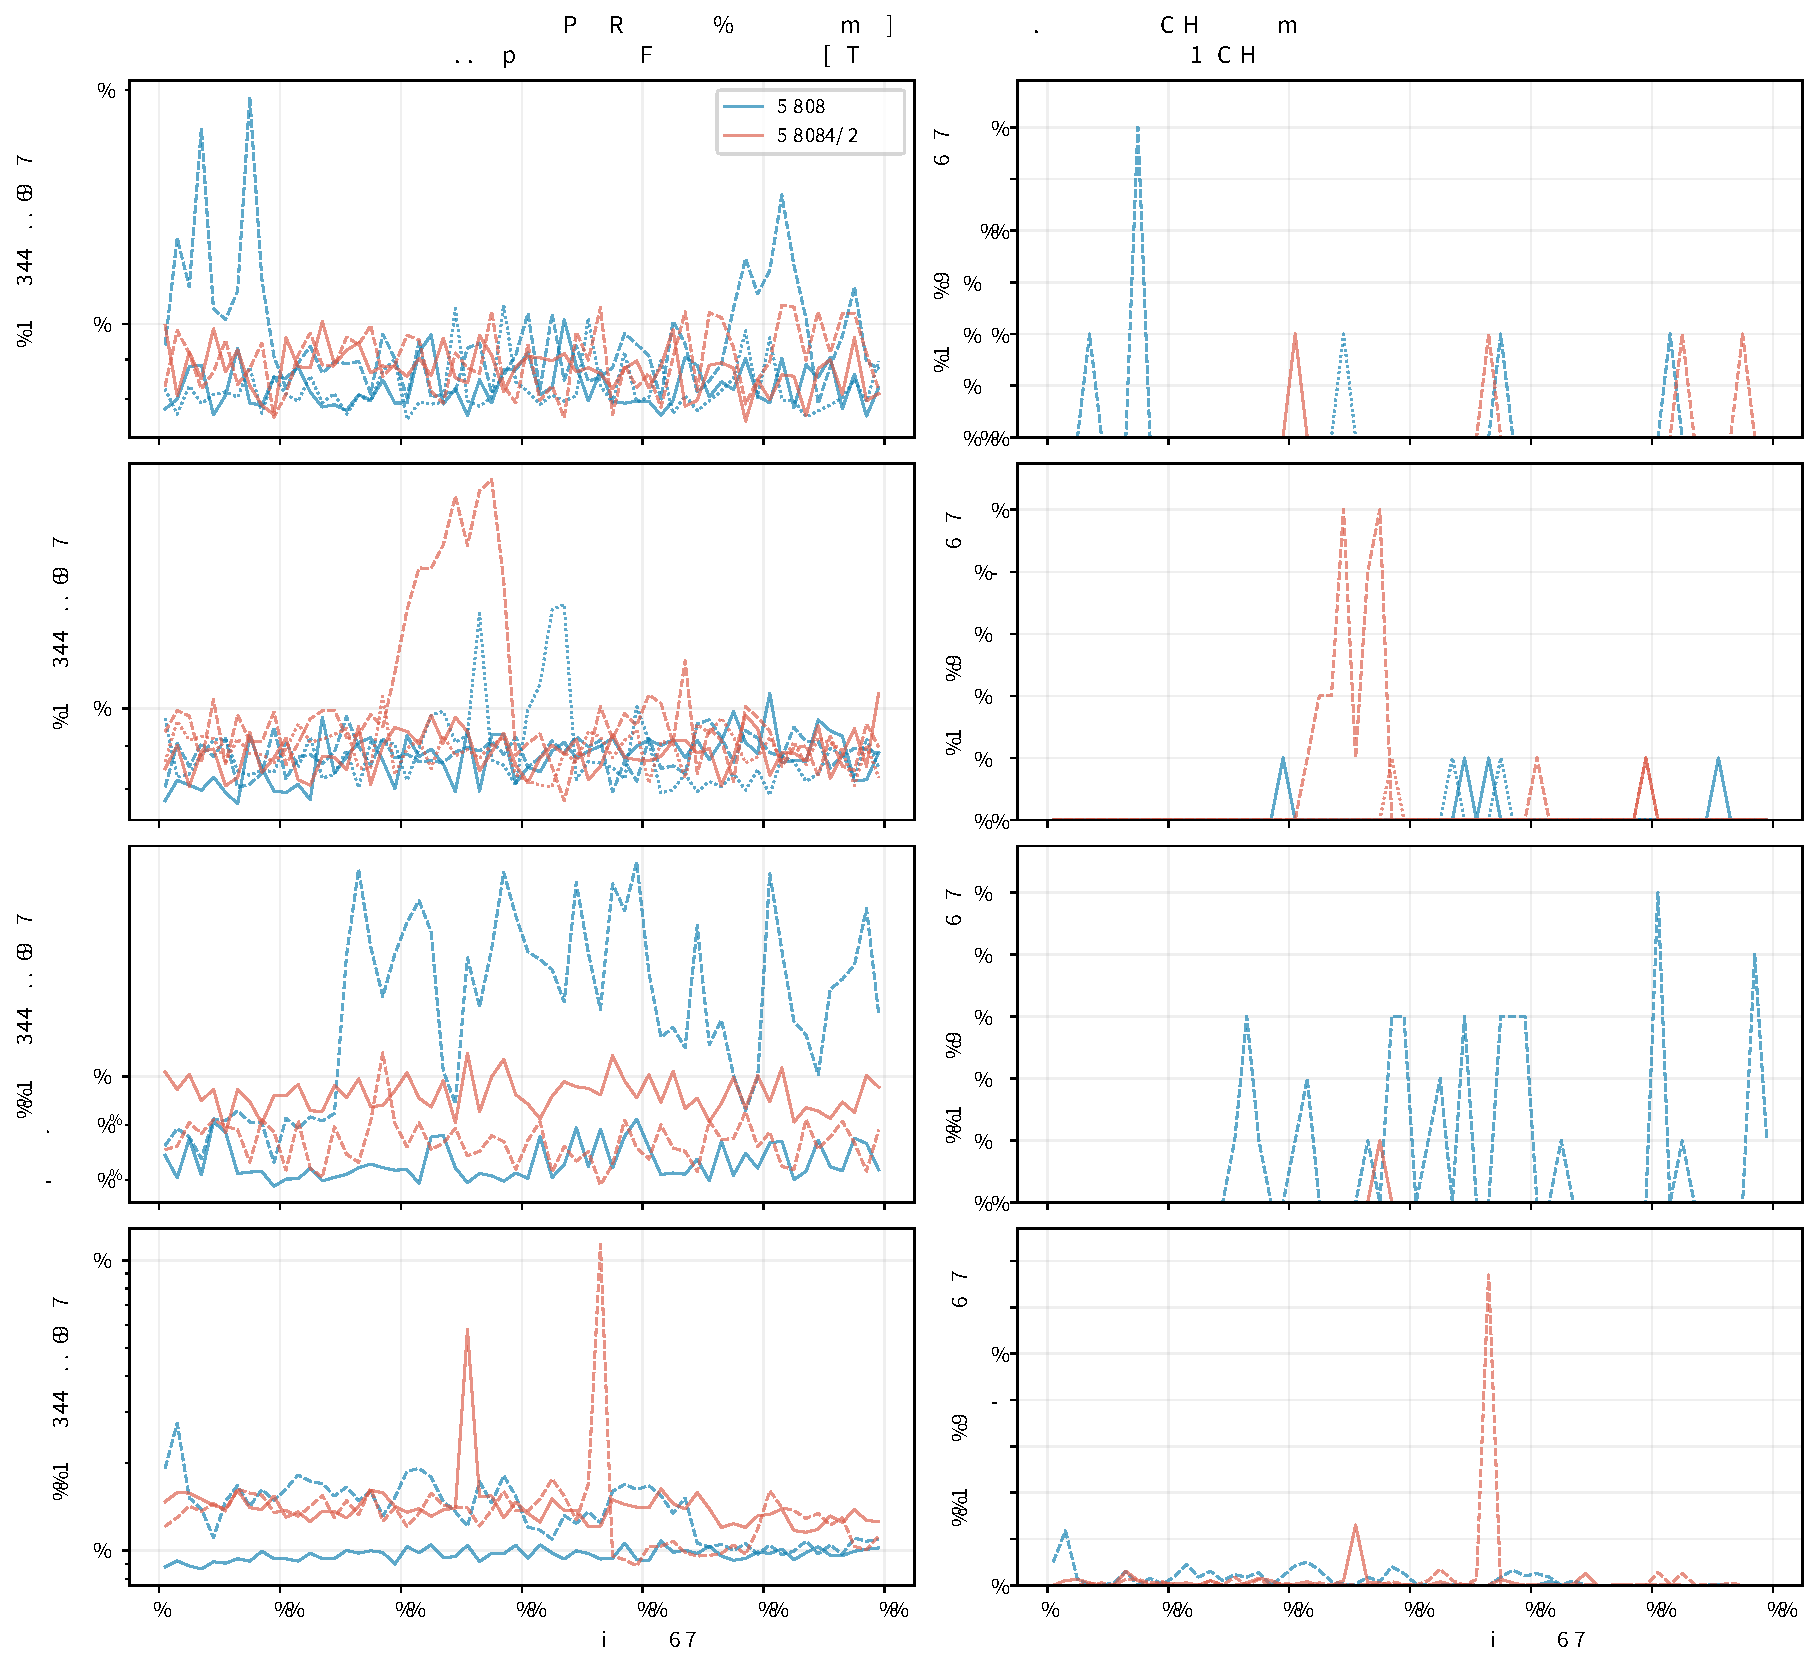
\includegraphics[width=\linewidth]{../experiments/figures/operational/espnow-long-timeline.pdf}\caption{10秒ごとの推移。縦軸の尺度は指令周期ごとに異なる。}\end{figure}
\begin{figure}[htbp]\centering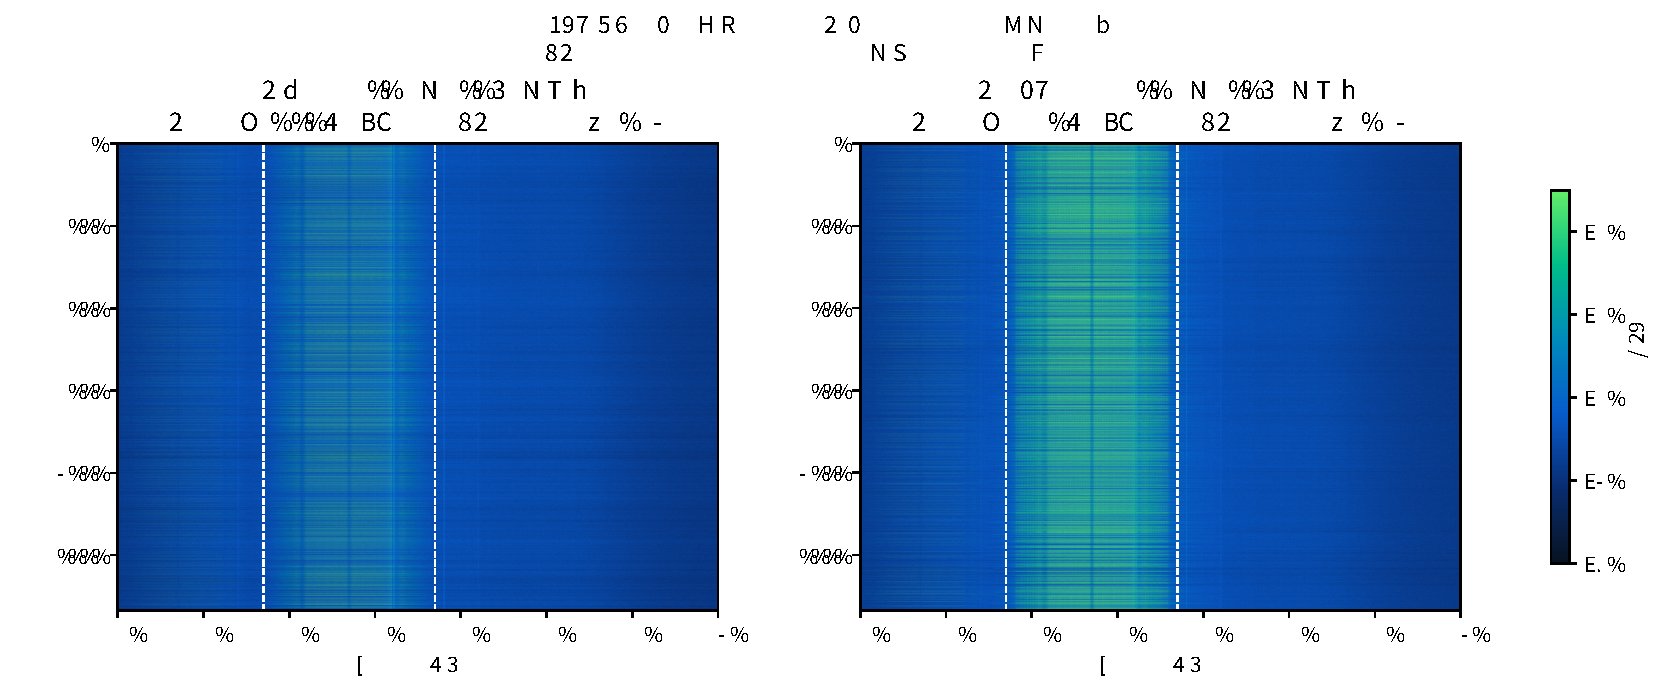
\includegraphics[width=\linewidth]{../experiments/figures/operational/espnow-long-blue-green.pdf}\caption{100 HzのWi-Fi待機と負荷、反復1。無線観測は間欠的である。}\end{figure}
\begin{figure}[htbp]\centering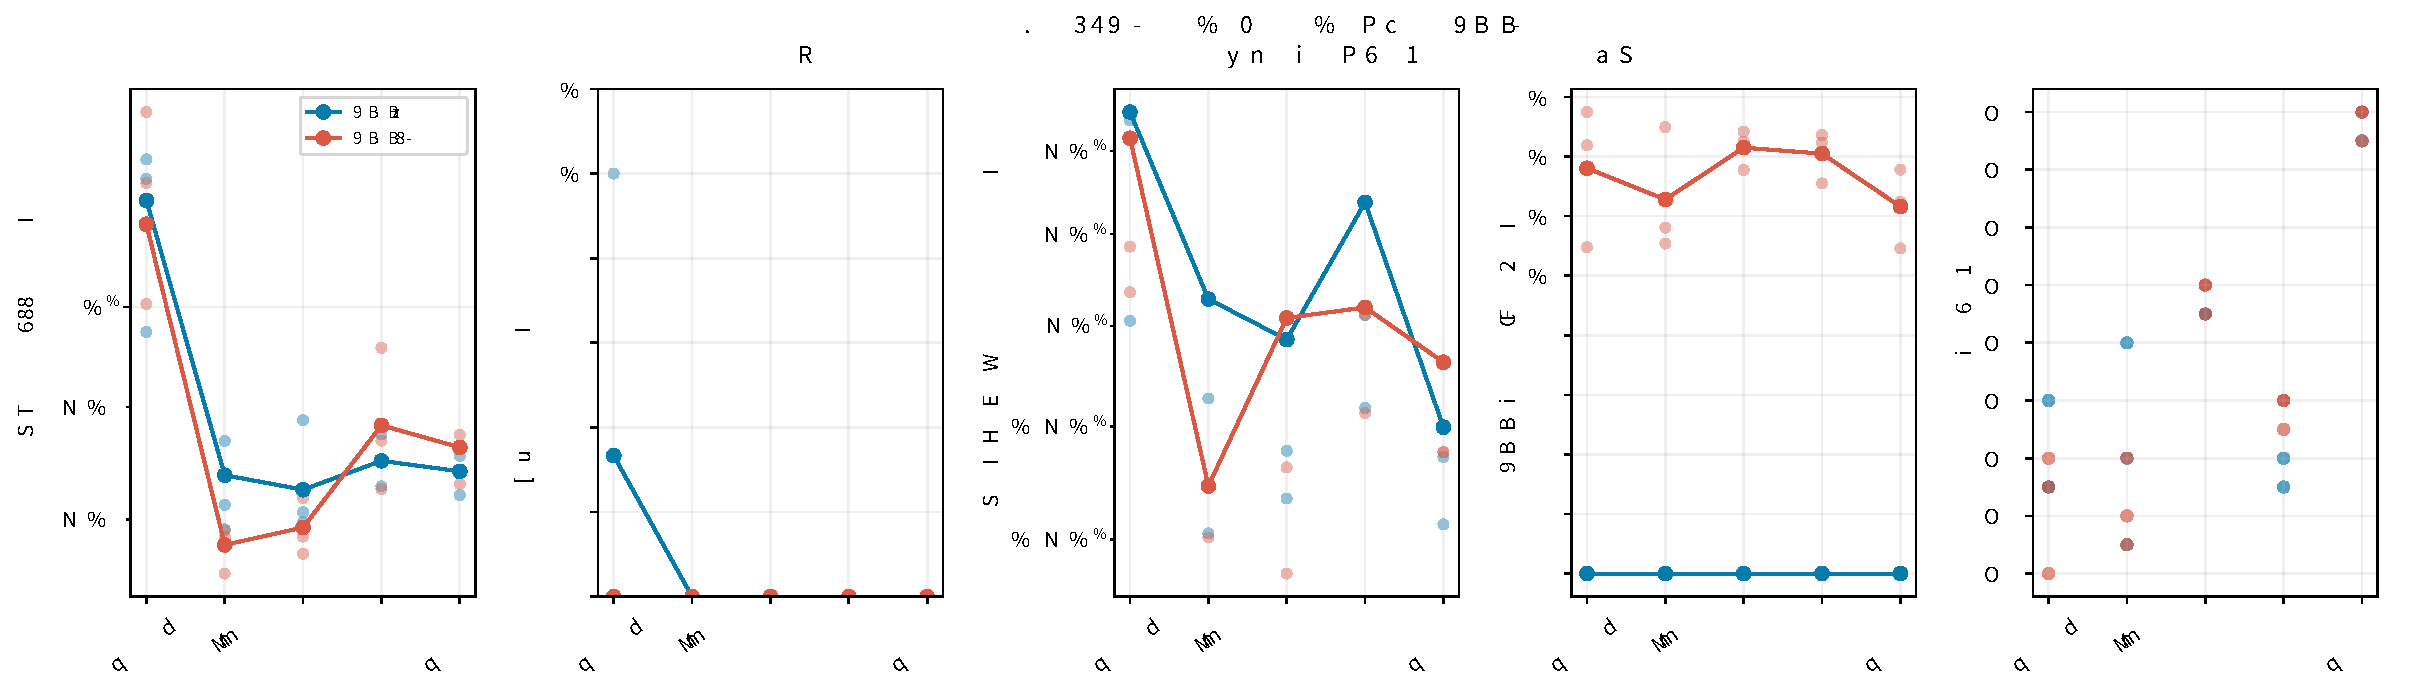
\includegraphics[width=\linewidth]{../experiments/figures/operational/placement-metrics.pdf}\caption{各10秒の手動配置比較。RSSIは届いた最新パケットの値。}\end{figure}
\begin{figure}[htbp]\centering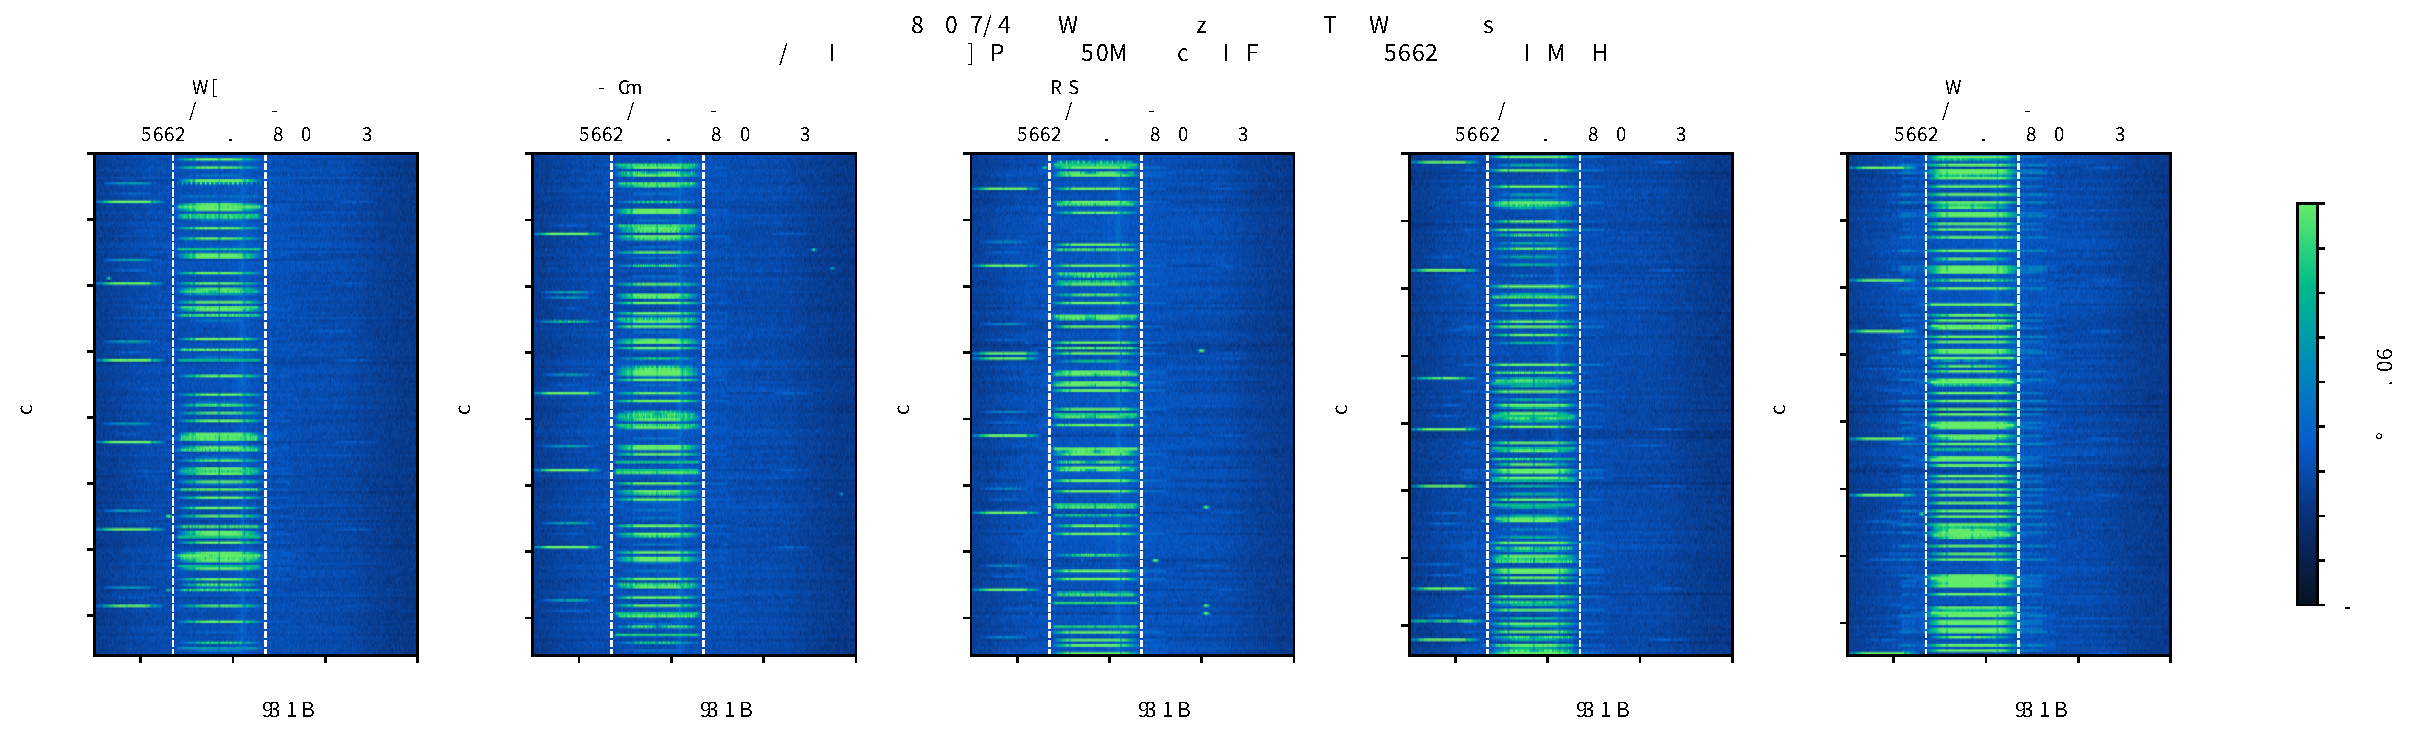
\includegraphics[width=\linewidth]{../experiments/figures/operational/placement-blue-green.pdf}\caption{各配置の負荷反復1。C5と応答機の距離も変化している。}\end{figure}
\clearpage\section*{先行通信実験とSDR受信評価}
% END OPERATIONAL STUDY
\section{主実験の通信構成}
本稿の主実験は、スマートフォンとロボットPCがルーターを通して指令・映像・点群を送る状況に近づけるため、UDPとTCPをいずれもSTA→AP→STAへ通した。自チームは観測PC（Intel BE200）をCh6・20 MHz AP、ESP32-3をコントローラー役、ラップトップ2（MT7921E）をロボットPC役とする。他チームはESP32-2 AP→ESP32-1 STAの独立した飽和TCP通信である。ラップトップ1（Intel AX210）のインターネット共有は有線で維持した。
\plot{../two-team/two-team-setup}{1}{主実験の構成。自チームの指令と大容量模擬データはAPによる無線中継を通る。}
実スマートフォン、ROS 2/DDS、実画像、点群内容、モーターは使っていない。100 Hz・64 byteのUDPを反射し、ESP32-3の同じ1 $\mu$s刻み時計で予定送信、実送信、応答時刻を記録する。RTTはアプリケーション往復時間で、片道遅延や制御応答ではない。3,000送信後に1秒の猶予を設け、返らなかった応答を欠落とする。p99は届いた応答だけ、20 ms期限超過は欠落も含む。20 msは比較用目標で安全停止のしきい値ではない。

大容量データは192 KiBを10 Hzで送ろうとする要求15.73 MbpsのTCP模擬負荷である。逆圧で送れない場合は送信側が待ち、要求速度を達成したとは扱わない。自チームの受信bytesは30 sの計測窓で数え、他チームは前後のカウンタ差とホスト区間で数えた。他チームの窓には終了猶予やテレメトリ取得も含まれ、窓は完全一致しない。自チームのデータは無線を2回、他チームは1回通るので、アプリケーションMbpsから同じ空中時間を仮定できない。

配置は同じ机上で固定し、使用者は各機器おおむね30 cmと報告した。個々の中心間距離と姿勢は先行系列で再確認しておらず、距離掃引ではない。自チーム負荷あり・なし、他チーム負荷あり・なし、Ch6・Ch7・Ch11の12条件に、両負荷のCh1・20/40 MHzを加えた14条件・3反復、計42試行を実施した。各30 s、各3,000送信、固定種で反復内の順序を無作為化した。他チーム待機にもAPビーコンとTCP接続は残す。

C5は80 MS/s、16,380 I/Q、48 MHzアナログ帯域、手動ゲイン20、FFT1024、DC除去とHann窓を使用した。全取得と時刻ダンプのCRC32を照合した。LOは2442 MHz、Ch1の幅比較だけ2427 MHz。dBFSは未校正で、RF観測時間比は約0.4\%。ESP時計とホストのUART開始時計は近似的に対応づけるため、パケット単位のI/Qとの一致判定には使わない。

\section{同一・隣接・分離チャネルの比較結果}
\begin{table}[htbp]\centering\small\caption{両チーム比較。各条件3反復9,000送信。自TCP・他TCPは各試行実受信Mbpsの範囲。期限は20 ms。}\begin{tabular}{llrrrrr}\toprule 自負荷 & 他条件 & p99 ms & 超過\% & 欠落\% & 自TCP & 他TCP\\\midrule
あり & Ch1/20/負荷 & 128.6 & 55.0 & 9.0 & 0.62--1.33 & 0.88--1.25\\
あり & Ch1/40/負荷 & 127.5 & 56.8 & 9.6 & 1.16--1.61 & 0.39--0.79\\
あり & Ch11/20/待機 & 126.5 & 54.4 & 10.6 & 0.97--1.35 & 0.00--0.00\\
あり & Ch11/20/負荷 & 127.4 & 57.2 & 11.3 & 1.18--1.41 & 1.00--1.28\\
あり & Ch6/20/待機 & 125.8 & 55.0 & 9.2 & 1.17--1.35 & 0.00--0.00\\
あり & Ch6/20/負荷 & 148.4 & 67.7 & 6.1 & 0.91--1.19 & 2.54--4.66\\
あり & Ch7/20/待機 & 123.8 & 53.8 & 9.8 & 1.02--1.31 & 0.00--0.00\\
あり & Ch7/20/負荷 & 132.3 & 63.0 & 7.0 & 1.19--1.45 & 2.34--3.79\\
なし & Ch11/20/待機 & 119.3 & 48.3 & 8.4 & 0.00--0.00 & 0.00--0.00\\
なし & Ch11/20/負荷 & 118.8 & 48.6 & 7.2 & 0.00--0.00 & 0.79--1.06\\
なし & Ch6/20/待機 & 117.3 & 47.0 & 5.9 & 0.00--0.00 & 0.00--0.00\\
なし & Ch6/20/負荷 & 131.2 & 54.6 & 5.5 & 0.00--0.00 & 3.96--4.63\\
なし & Ch7/20/待機 & 120.2 & 49.1 & 9.8 & 0.00--0.00 & 0.00--0.00\\
なし & Ch7/20/負荷 & 124.4 & 50.8 & 6.6 & 0.00--0.00 & 3.14--3.85\\
\bottomrule\end{tabular}\end{table}
\plot{../two-team/two-team-blue-green}{1}{同一・隣接・分離の実測スペクトル。各画像は1反復目、RTT注記は3反復統合値。白破線は自チームの名目帯域、色尺度とゲインは共通。}
自チーム大容量通信中、他チームの負荷によるp99の増分はCh6で22.6 ms、Ch7で8.6 ms、Ch11で0.9 msだった。20 ms期限超過の増分も同一・隣接で大きい。一方、欠落率は両負荷Ch6/Ch7で待機より小さく、欠落だけで通信の良否を判定すると期限超過の悪化を見落とす。p99も受信応答に条件づけた指標なので、欠落と併せて評価する。

Ch6とCh7の中心差は5 MHzで20 MHz幅の通信は大きく重なる。画像で重なる領域と、Ch11で分かれる領域を見られる。ただし同一Ch6が今回最も遅く、部分重複がいつでも最悪とは言えない。同一チャネルの送信待ち、部分重複の受信妨害、RF再送、APや端末の処理は候補になる\cite{ciscoRF}が、今回の測定はそれらを原因分離していない。他チームの受信量もCh6約2.5--4.7、Ch7約2.3--3.8、Ch11約1.0--1.3 Mbpsと異なり、等しい空中時間の周波数比較ではない。

\subsection{単独通信時の基準性能と干渉評価}
操縦のみ・他待機でもp99は117--120 ms、20 ms期限超過は47--49\%であり、この系は既に目標を満たさない。自チーム模擬TCPは要求15.73 Mbpsに対して約0.6--1.6 Mbpsしか到達していない。これは今回の構成の処理・伝送限界を含む値で、競技用ルーターやPC同士のROS 2の上限を示すものではない。他チームの効果は同じ自負荷・他チャネルの待機との差として論じ、全遅延を干渉へ帰属しない。ユーザーが使う実システムでは、まず単独で期限を満たす基準を作り、双方が実負荷を流した時の差を見る手順が有用である。
\plot{../two-team/two-team-interaction}{1}{各反復のp99と統合期限超過。自負荷なし・ありを分け、他負荷の効果と反復変動を確認する。}

\section{チャネル幅と操縦通信性能}
\plot{../two-team/two-team-width}{1}{他チームCh1の20/40 MHz。クライアントの接続幅と副チャネルを読み出した。}
Ch1の20 MHzとCh6は名目帯域が分かれるが、上側副チャネルを加えた40 MHzはCh6へ重なる。主実験の統合p99は20 MHz 128.6 ms、40 MHz 127.5 ms、期限超過はそれぞれ55.0\%、56.8\%だった。p99の明確な悪化は確認しなかった。他チーム実受信量も20 MHz約0.9--1.2、40 MHz約0.4--0.8 Mbpsと違うため、「広いほど速い」「広いほど必ず操縦が悪い」のどちらもこの結果から言えない。

幅の拡大は1送信あたりの情報量と隣のリンクへ残る帯域の両方を変える\cite{ciscoRF}。実接続40 MHzでも全パケットが40 MHz波形になるとは限らない。重なりを避けやすい設定と、実際に期限を守る設定を区別し、自分の通信負荷と他チーム負荷の組で測る必要がある。

\section{通常Wi-Fiの周期負荷による意図的なストレス試験}
自チームの大容量通信を保ち、他チームの通常TCP負荷を2 s ON・2 s OFFで操作した。Ch6・Ch7・Ch11、各3反復、計9試行。UARTコマンドの前後時刻と実受信bytesを保存した。所有リンクへの通常のデータ通信を使った試験である。
\plot{../two-team/wifi-burst-blue-green}{1}{周期負荷の実測FFTと同じ試行のRTT。緑帯はON操作区間で、RF送信の厳密な開始時刻ではない。}
\begin{table}[htbp]\centering\small\caption{周期負荷30 s全体。ON/OFFを含み、各9,000送信。}\begin{tabular}{lrrr}\toprule 条件 & p99 ms & 20 ms超過\% & 欠落\%\\\midrule
周期負荷 Ch6 & 143.3 & 68.2 & 7.4\\
周期負荷 Ch7 & 128.5 & 58.2 & 9.6\\
周期負荷 Ch11 & 128.7 & 57.7 & 9.1\\\bottomrule\end{tabular}\end{table}
TCP送信は負荷ONでもバーストや再送を含み、連続したRFではない。画像の取得窓と指令の時刻対応は近似であり、個々のパケットがどのRFへ妨げられたかは特定していない。欠落した応答はRTT点として図に出ないため、遅い点の減少だけを改善と扱わない。実装上の波形ON/OFF操作と、通信性能を同時に記録する例として位置付ける。

\section{独立したBluetooth LEリンクとの比較}
ESP32-1/2をBLE専用送受信機へ切り替え、Wi-Fi端末とAPは保った。BLE停止、20 ms設定の非接続広告、BLE 1MのGATT通知を、自チーム大容量通信なし・ありで各3反復、計18試行比較した。広告は受信側で実際の復号回数、通知は受信bytesと件数を残す。GATT MTU、接続間隔、送信API受付量とエラーも読み出した。BLEの負荷を2 ms周期で要求するが、実到達量は受信カウンタで評価する。送信APIの受付エラーはスタックの逆圧も含み、PHYパケット損失率へ読み替えない。
\plot{../two-team/ble-blue-green}{1}{BLE停止・広告・通知と、自チームWi-Fi大容量通信の有無。実測FFTを共通色尺度で表示。}
\plot{../two-team/ble-narrow-blue-green}{1}{Ch6の上側2450--2470 MHzを拡大。弱い成分を読むため、この図内で共通の$-90$--$-60$ dBFS尺度を使用する。前図とは同じ色が同じ電力を示さない。細線の全てをBLEへ帰属しない。}
\begin{table}[htbp]\centering\small\caption{外部BLEとWi-Fi操縦性能。BLE受信は試行平均Mbps。広告は復号件数を個別JSONに保存。}\begin{tabular}{lrrrr}\toprule 条件 & p99 ms & 20 ms超過\% & 欠落\% & BLE受信\\\midrule
操縦 / BLE停止 & 118.9 & 49.2 & 8.6 & 0.00\\
操縦 / BLE広告 & 118.4 & 47.5 & 6.8 & 0.00\\
操縦 / BLE通知 & 121.6 & 48.6 & 6.6 & 0.36\\
重負荷 / BLE停止 & 126.2 & 54.6 & 8.1 & 0.00\\
重負荷 / BLE広告 & 126.0 & 58.2 & 9.3 & 0.00\\
重負荷 / BLE通知 & 126.3 & 56.8 & 9.3 & 0.33\\
\bottomrule\end{tabular}\end{table}
Wi-Fi大容量通信中のp99はBLE停止126.2 ms、広告126.0 ms、通知126.3 ms。BLE通知の実受信量はWi-Fi待機0.36 Mbps、Wi-Fi負荷0.33 Mbpsだった。Wi-Fiの悪化だけを探すのでなく、BLE側の受信量と両方式の性能を併せて見る比較である。今回のBLE追加ではWi-Fiのp99が大幅に増える結果ではなかったが、BLE通知の実受信量はWi-Fi負荷の有無で変わった。どちらのリンクへ影響が出るかは、方式と負荷の組合せで確認する必要がある。因果評価には同じ方式・負荷・配置の反復が必要で、この少数反復の室内結果からBluetooth全般を無害または有害と決めない。



% BEGIN BLE CHANNELS
\subsection{広告と接続通信で異なるチャネルの使い方}
周波数ホッピングは、送受信機が約束した順序で使用周波数を時間とともに切り替えることである。
周波数帯全体へ同時に広い信号を送ることではない。BLEは2.4 GHz帯に2 MHz間隔の40チャネルを持ち、
今回使ったlegacy広告には2402・2426・2480 MHzの3広告チャネル、接続後の通信には37データチャネルを使う\cite{blePrimer}。
したがって「広告をONにした」と「接続後のホッピング通信を高負荷で動かした」は別の条件である。

GATT通知のような接続通信では、接続イベントの開始ごとに両端が同じデータチャネルを選ぶ。
1つのイベント中の全パケットが毎回別周波数へ飛ぶという意味ではない。
AFH（適応的周波数ホッピング）は、使用するチャネルの集合を更新し、通信しにくい周波数を避ける仕組みである\cite{bleAFH}。
一方、今回のlegacy広告は3広告周波数を使用し、接続後と同じ37チャネルのAFHとして扱わない。
今回、チャネルマップや更新時刻を取得していないため、Wi-Fiを検出して特定チャネルを除外したかは確認していない。

\subsection{ホッピングしてもWi-Fiと干渉し得る理由}
Wi-Fi Ch6の中心は2437 MHz、名目20 MHzの範囲は2427--2447 MHzである。
その内部にもBLEデータチャネルがある。BLEがそこへホップした時にWi-Fiも同時送信すれば、
周波数と時間が重なり、受信失敗や再送につながり得る\cite{bleAFH}。
ホッピングは同じ悪い周波数へ留まり続けることを減らすが、全ての送信をWi-Fiから切り離す仕組みではない。
影響は重なる周波数だけでなく、送信の頻度・長さ、両送信機の強さ、受信側での信号対干渉比によって変わる。

Wi-Fiの幅を20から40 MHzへ広げると、BLEと重なり得る周波数の範囲も広がる。
ただし達成レートが上がれば同じデータを短時間で送り終える可能性もあるため、幅だけで衝突回数や劣化量は決められない。
今回の幅比較は別チームWi-Fi同士の実験であり、BLEとの共存を20/40 MHzで直接比較した実験ではない。
これは今回の観測を読むための機構説明で、幅とBLE干渉の因果効果を測定したという主張ではない。

\subsection{Wi-FiからBLEへ、BLEからWi-Fiへの実測変化}
Wi-Fi大容量通信中のRTT p99は、BLE停止・広告・通知の順に126.18／126.00／126.32 msと近い。一方、20 ms期限超過は54.57／58.16／56.81\%、Wi-Fiの実受信平均は1.340／1.496／1.189 Mbpsだった。
BLE通知の実受信平均は、Wi-Fi待機時0.365 Mbpsから負荷時0.326 Mbpsへ変化した。

したがって「Wi-Fi p99がほぼ同じなので影響なし」とは言えない。
指令の期限超過、Wi-Fiの配送量、BLE側の配送量を別々に見る必要がある。
同時に、各条件3反復で実負荷も変動しており、この変化を全てRF衝突やAFHの効果へ帰属できない。
通知の受付エラーも無線衝突数ではない。干渉機構を同定するには、再送、チャネルマップ、
周波数ごとの失敗を対応付ける記録が必要で、今回は取得していない。

図の短い細線は、広帯域Wi-Fiと異なる狭帯域送信を読む手掛かりである。
ただしC5の取得は間欠的で、図は2450--2470 MHzの一部のみを拡大している。
広告の3周波数はいずれもこの拡大範囲の外であり、広告の図で帯が見えないことは送信停止の証拠ではない。
全ての細線をBLEと同定したり、ホッピングの連続した軌跡やAFHで避けたチャネルを図から復元したりはできない。
同一チップ内の無線資源の共存制御、Bluetooth Classic、音声通信とは分けた実験である。
% END BLE CHANNELS

% BEGIN ESPNOW STUDY
\section{ESP-NOWの指令と独立したWi-Fi大容量通信}
ESP32-1からESP32-2へ64 byte・100 Hzの未暗号化unicast指令を送り、受信タスクが同じ内容をアプリ応答として返す。APを通らない経路である。Wi-Fi側は観測PC（Intel BE200）Ch6・20 MHz APに固定し、ラップトップ2からESP32-3へ大容量TCP模擬データを流す。ESP-NOWをCh6・Ch7・Ch11へ動かし、Wi-Fi待機・負荷の6条件、各30 s・3反復、18試行を実施した。条件順は反復内で無作為化した。

ESP-NOWは1 Mbps・long preambleへ明示設定し、受信metadataのrate=0、sig\_mode=0を両端で確認した。PHY設定と受信結果を区別して残す。MACの送信成功はアプリ応答の成功ではない\cite{espnowGuide}ため、後者のRTTと欠落を測り、送信callbackの成功・失敗、APIエラー、echoキューの取りこぼしも保存した。アプリ再送は行わない。API受付失敗も送信要求の分母に含め、応答欠落を物理層の損失率へ読み替えない。時刻列は送信側の同じµs時計で、終了後1 sを応答猶予とする。UART115200によるCRC付き読み出しは測定後に行い、RTTへ含めない。Wi-Fi受信量には読み出しを含むカウンタ区間の実時間を使う。

配置は同じ机上で固定した。先行記録の距離は個々の中心間距離を再確認していない。送受信機、無線経路、PHYがAP中継のUDP比較と異なるので、その差をESP-NOWという方式だけの因果効果として扱わない。C5の80 MS/s・48 MHz・ゲイン20・FFT1024・LO2442 MHzは同じで、間欠取得と未校正dBFSの制約も同じである。
\begin{table}[htbp]\centering\small\caption{ESP-NOW操縦応答。表のChはESP-NOW側、Wi-Fi APはCh6固定。各9,000送信。Wi-Fi実受信は試行範囲Mbps。}\begin{tabular}{lrrrr}\toprule Wi-Fi / ESP-NOW & p99 ms & 20 ms超過\% & 欠落\% & Wi-Fi Mbps\\\midrule
待機 / Ch6 & 9.4 & 0.1 & 0.00 & 0.00--0.00\\
待機 / Ch7 & 14.5 & 0.4 & 0.00 & 0.00--0.00\\
待機 / Ch11 & 288.5 & 15.4 & 0.32 & 0.00--0.00\\
負荷 / Ch6 & 85.6 & 4.7 & 0.02 & 1.11--1.45\\
負荷 / Ch7 & 18.4 & 0.6 & 0.00 & 1.06--1.37\\
負荷 / Ch11 & 91.1 & 20.5 & 0.46 & 1.22--1.37\\\bottomrule\end{tabular}\end{table}
\plot{../espnow/espnow-blue-green}{1}{ESP-NOWとWi-Fiの実測RF。各画像は1反復目、注記は3反復統合値。Wi-Fiの名目帯域を白破線で示す。}
Wi-Fi負荷を加えた時、ESP-NOWの統合p99は同一Ch6で9.4→85.6 ms、隣接Ch7で14.5→18.4 ms、分離Ch11で288.5→91.1 msだった。数値の比較には欠落と期限超過も使い、遅い応答が欠落したことによる見かけのp99低下を改善と扱わない。各反復p99は公開JSONに残し、9,000パケットを9,000の独立な環境反復とはみなしていない。Ch11待機の各反復p99は37.0--341.3 msとばらついた。分離Ch11にも待機状態で大きな遅延があり、今回の結果は「周波数を離すと常に良い」ではない。試験用Wi-Fiを止めても室内の他の送信機やリンクの状態は残る。外来通信、受信余裕、送信待ち、処理のどれが主因かは今回分離していない。

\plot{../espnow/espnow-repeat-variation}{1}{同一Ch6・Wi-Fi負荷の全3反復。下段は届いた応答のRTT、赤破線は20 ms。欠落は点として現れない。上段と下段はUART開始時刻に基づく近似対応であり、パケット単位の時刻相関ではない。}
同じCh6・負荷ありでも反復p99は8.6--123.8 msだった。1・2反復目では20 ms期限超過が0\%、3反復目では14.1\%に増えた。チャネルと負荷設定を固定しても尾部遅延は再現しなかった。Wi-Fi実受信も変わるため、一定の干渉強度を与えた比較ではない。単独基準、反復、期限超過、応答途絶を組み合わせ、1回の平均速度やスペクトルの見栄えから指令品質を判断しないことが実践上の学びである。原因を処理待ちとRF干渉へ分解するには、追加の処理時刻と送受信フレームの観測が必要となる。

全54,000送信要求に対し、送信側API受付エラー23、送信側MAC失敗36、echo側MAC失敗68を記録した。echoキューの取りこぼしは0だった。これらはパケットごとの因果対応を持たず、合計をそのままアプリ応答欠落へ割り当てない。


% BEGIN ESPNOW CHANNELS
\subsection{ESP-NOWの固定チャネルとBLEとの相違}
ESP-NOWはWi-Fiの無線部からvendor-specific action frameを直接送る方式であり、
標準でBLEのような自動的な周波数ホッピングを行う方式ではない\cite{espnowGuide}。
今回のESP32送受信機は2.4 GHzの同じWi-Fiチャネルに合わせて動作させた。
peerのchannel=0は現在の無線チャネルを使う指定であり、空いている周波数を自動探索する指定ではない。
送受信機のチャネルが一致しなければ通信できない。

先行試験ではCh6・Ch7・Ch11へ試行間で切り替え、それぞれの30秒試行中は固定した。
これはホッピング実験ではなく、試行ごとに設定した固定チャネルの比較である。
後続の600秒試験と配置比較は、ESP-NOWと別系統Wi-FiをともにCh6へ固定した。
試行前後の実チャネル読出しと取得コードでこの設定を確認しており、途中で自動的に干渉を回避した結果とは解釈しない。

\subsection{ルーターを経由しなくてもWi-Fiと干渉し得る理由}
ESP-NOWはAPによる中継を省けるが、同じ周波数帯の送信時間から独立するわけではない。
同一または重複チャネルのWi-Fiと同時に使うと、送信待ちや受信失敗・再送が増える可能性がある。
Ch6とCh7は中心周波数が5 MHzしか離れず、チャネル番号が違っても帯域は大きく重なる。
1 Mbpsは今回設定したPHYのbitrateであり、電波の占有幅が1 MHzという意味ではない。

別の無線機同士なら、自チームWi-FiとESP-NOWへ分離したチャネルを割り当てる構成を検討できる。
一方、同じESP32の無線部でAPへのWi-Fi接続も併用する場合、ESP-NOWのチャネルを接続APに合わせる必要がある\cite{espnowFAQ}。
その構成で「Wi-FiはCh6、ESP-NOWはCh11を同時に固定する」とは設定できない。
今回の独立した無線機によるチャネル比較と、同一チップ内の併用を区別する必要がある。

\subsection{Wi-Fiとの相互影響について今回言えること}
先行30秒試験では、Wi-Fi負荷を加えると同一Ch6のESP-NOW RTT p99が9.4から85.6 msへ変わった。
ただし同じCh6負荷中でも反復p99は8.6--123.8 msと変動した。
後続600秒試験では100 Hz・Wi-Fi待機から負荷へのp99が10.711から9.264 msであり、
同一チャネルなら必ず同じ量だけ悪化するという結果ではない。
実装・測定時間・配置の異なる系列をまとめず、指令の期限超過と最長更新途絶も比較する。

逆方向については、共存中のWi-Fi実受信量も保存したが、ESP-NOWを停止した同一条件のWi-Fi単独基準は測っていない。
したがって「ESP-NOWがWi-Fiを何\%遅くした」「Wi-Fiへ影響しない」は今回の記録から定量的に断定できない。
これはWi-Fi負荷の中でESP-NOW指令が間に合うかを中心に評価した実験である。
また指令とその応答はどちらも無線時間を使い、指令周期を短くするとヘッダ・応答・送信待ちも増える。
小さいpayloadのMbpsだけを見て無視できる負荷と決めず、映像と同時に動かして指令更新の尾部を調べることがロボコンでは有用である。
% END ESPNOW CHANNELS

\subsection{ロボコンへの適用条件}
AP経路を外した小さい指令でも同じ2.4 GHz帯を使い、外部Wi-Fiが動作する配置で評価する必要がある。1 Mbpsはbitrateで、電波の幅が1 MHzという意味ではない。小さい指令でも帯域幅を持つ成分として観測される。今回のESP-NOWは64 byteの指令試験であり、映像や点群を運ぶ大容量転送の性能を測っていない。ROS 2トピックがそのままESP-NOWになる実装でもなく、PCやコントローラーとの橋渡しは別途必要で、その遅延は今回含まない。同じESP32無線にWi-Fi接続とESP-NOWを併用する場合、接続APとpeerのチャネル条件を考慮する必要がある\cite{espnowGuide}。今回の独立無線によるチャネル分離結果をそのまま同一チップへ適用しない。

距離、向き、移動、暗号化、通信途絶時の停止動作は未比較である。無線が接続しているかより、届いた指令の新しさと途絶を判断する方法が検討対象になるが、本測定だけで安全な停止期限を決められない。
% END ESPNOW STUDY
\section{主実験の結論}
両チームが負荷を流す今回の固定配置では同一・隣接チャネルで操縦期限超過が増え、分離Ch11では増分が小さかった。帯域の重なりをSDRで見ながら、待機との差、実受信量、RTTと欠落を同時に比較する方法を示した。ただし主リンクの単独基準も不良であり、端末構成とRFを原因分離せずに競技場へ外挿できない。帯域幅の比較は単調な悪化を示さず、Bluetooth比較も指定のBLE負荷と配置に限定する。

ロボコンでは単独時の期限をまず満たし、自分の映像・点群と他チーム通信を同時に動かす。その時の期限超過や最長応答間隔に基づいて、負荷制限・古い指令の破棄・通信途絶の検出などを検討する。それらの改善効果と安全な停止しきい値は本実験では検証していない。


\clearpage
\section{先行実験の位置付けと構成の相違}
以下は先行56通信試行と115受信観測系列を保持した補足である。先行の別AP比較では主リンクが操縦中心であり、本稿前半の両チーム負荷とSTA→AP→STA構成とは異なる。数値を同じ群へ統合せず、設定依存性とSDR画像の読み方を支える結果として参照する。先行BLE観測だけでは性能劣化を評価していなかったが、前半には独立BLEリンクとWi-Fi性能の同時比較を追加した。
% END TWO TEAM STUDY
\section{操縦通信の無線品質評価}
ロボットの操縦では、平均転送速度だけでなく、古い指令が届くまでの待ち時間と、応答が途切れる時間が問題になる。本実験は64 byteのUDPを100 Hzで送り返す通信を用い、映像相当のTCP負荷、別APのチャネル、チャネル幅、送信電力設定を変えた。主題は\textbf{ロボコンで通信設定を選ぶために、周波数の重なりと操縦通信の遅延を対応づけること}である。実際のロボット・映像コーデック・モータ制御は使っていない。

平均速度を増やした時に遅延の裾が伸びるか、スペクトルの重複と操縦応答の劣化が対応するか、幅を広げることで隣の通信への影響が変わるかを、別々の比較で調べる。干渉を断定する前に待機状態の基準値を取り、端末側の遅延をRFの効果と取り違えないようにした。

\section{実験系と評価方法}
観測PC（Intel BE200）をCh6・HT20のWPA2 APとし、ラップトップ1（Intel AX210）から有線LANでインターネット共有を受けた。ESP32-1（ESP32-D0WD）は全主比較でこのAPのSTAとなり、操縦UDPを反射する。ESP32-2（ESP32-PICO-D4）は独立したAPとTCP送信機となる。ラップトップ2（MT7921E）は、同一AP比較では観測PCからTCPを受信し、独立AP比較ではESP32-2へ接続してTCPを受信する。後者の期間はラップトップ2のインターネットを使わず、自律スクリプトで復帰させた。観測PCの有線インターネットは維持した。

同一AP負荷比較ではhostapd、独立AP比較の主APではNetworkManagerを使った。実接続はどちらもCh6・20 MHzだがAP起動設定は完全に同一ではないため、\textbf{各比較群の待機条件を基準とする}。同一AP負荷と独立AP負荷の数値差を、負荷の置き場所だけの効果として解釈しない。

配置は同じ机上で固定し、使用者は各機器おおむね30 cmと報告した。各中心間距離と姿勢はこの先行系列では実測していない。後続の手動配置比較の距離を遡って代入しない。\textbf{物理距離を変えた近接・遠方の比較ではない}。送信電力設定の比較を距離掃引や校正済み入力レベル掃引とは呼ばない。

1試行30 s、3,000 UDP指令、基本3反復とした。省電力の補助比較は2反復である。反復ごとに条件順序を乱数種固定で変更し、同一AP比較と独立AP比較の順序自体は固定した。評価はアプリケーションの送信から同じ内容の応答を受けるまでの\textbf{往復遅延（RTT）}、欠落率、20/50 ms以内に応答しなかった割合、最長応答間隔である。欠落も期限超過へ含める。最長応答間隔は30 sの測定開始・終了を含み、終了後1 sの待機で届いた応答も欠落判定には使う。p99は受信できた応答について計算し、欠落率を併記する。

RTTは片道の指令到着遅延でも、実ロボットの制御応答でもない。RTTを2で割って片道値にしない。送信予定時刻と実送信時刻を保存して、ホストの送信遅れも確認した。各試行のp99と全反復をまとめたp99を残し、パケットを独立な反復数とみなした信頼区間は作っていない。

C5は80 MS/s、16,380組の8+8 bit I/Q、48 MHzアナログ帯域、手動ゲイン指数20で、UDPと並行して約30 s取得した。全取得のCRCを照合した。FFTはDC除去、Hann窓、窓和二乗による規格化、線形電力平均を用いる。dBFSは絶対電力に校正していない。Ch1の幅比較はLO=2427 MHz、他の独立AP比較はLO=2442 MHzとした。表示スパン80 MHzでも感度は均一ではなく、異なるRF位置の高さから送信電力を直接比較できない。

\section{同じAP内での操縦と動画相当通信}
\begin{table}[htbp]\centering\small\caption{同一AP比較。省電力条件以外は3反復・各9,000応答機会。PSは2反復・6,000機会。期限超過には欠落も含む。}\begin{tabular}{lrrrrr}\toprule
条件 & p50 ms & p99 ms & $>20$ ms \% & 欠落\% & 最長間隔ms\\\midrule
待機 & 3.9 & 10.6 & 0.00 & 0.00 & 24.5\\
20 Mbps指定 & 4.4 & 21.0 & 1.32 & 0.00 & 48.8\\
60 Mbps指定 & 7.3 & 36.9 & 7.42 & 0.00 & 102.9\\
20 Mbps＋PS & 4.5 & 21.4 & 1.38 & 0.05 & 97.6\\
\bottomrule\end{tabular}\end{table}


待機状態の統合p99は\SameIdlePninetyNine{} ms、20 Mbps指定では\SameTwentyPninetyNine{} ms、高負荷では\SameHighPninetyNine{} msとなった。高負荷の20 ms期限超過率は\SameHighDeadline{}\%、最長応答間隔は\SameHighGap{} msである。主要3条件の欠落率は0\%であった。\textbf{全パケットが届くことと、操縦周期に間に合うことは別の性質である。}100 Hzの送信間隔は10 msなので、高負荷時の最長応答間隔は約10周期に相当する。ただしこれは応答の途絶であり、ロボットへの片道指令が同じ時間途絶したという意味ではない。

中央値の増加よりp99の増加が大きく、平均的な応答だけでは遅いバーストを見落とす。TCP指定速度を上げても実効速度は頭打ちになった一方、遅延の裾は伸びた。この結果は、操縦と映像が同じ媒体・APの処理・送信待ちを共有することと整合する。RF再送、AP内の待ち行列、TCPのバースト性、端末処理を本計測だけで分離したわけではない。

実用上は映像の平均Mbpsだけでなくピークの送信量を抑え、操縦の期限超過率を同時に見る意味がある。送信が詰まった際に古い操縦値を蓄積しない設計、最新値の優先、期限切れの破棄、通信途絶時の停止判断は候補となる。本実験ではそれらの制御方式や優先度設定の改善効果を比較しておらず、観測した約103 msを安全な停止しきい値として提案しない。

省電力比較はp99だけでは明確な改善・悪化の一方向を示さなかった。2試行のうち1試行で3応答が欠落し、統合欠落率は0.05\%だった。送信の頻度、受信機の省電力状態、AP側バッファリングが影響し得るが、2反復で省電力一般の因果効果を確定しない。

\section{独立した別AP：同一・部分重複・分離チャネル}
\begin{table}[htbp]\centering\small\caption{独立AP比較。各3反復・9,000応答機会。RTT分位点は受信できた応答の統合値。}\begin{tabular}{lrrrrr}\toprule
条件 & p50 ms & p99 ms & $>20$ ms \% & 欠落\% & 最長間隔ms\\\midrule
Ch11待機 & 3.7 & 10.8 & 0.02 & 0.00 & 33.0\\
Ch6待機 & 3.7 & 10.2 & 0.06 & 0.00 & 43.1\\
Ch7待機 & 3.7 & 10.4 & 0.03 & 0.00 & 27.1\\
Ch6負荷 & 4.2 & 26.5 & 1.77 & 0.00 & 68.3\\
Ch7負荷 & 4.0 & 15.6 & 0.26 & 0.00 & 40.4\\
Ch11負荷 & 3.8 & 13.1 & 0.16 & 0.00 & 42.6\\
Ch1 HT20負荷 & 3.8 & 13.8 & 0.19 & 0.00 & 44.3\\
Ch1 HT40負荷 & 4.0 & 20.0 & 1.00 & 0.00 & 62.6\\
Ch7低電力負荷 & 3.9 & 15.1 & 0.24 & 0.00 & 39.3\\
\bottomrule\end{tabular}\end{table}

\begin{figure}[htbp]\centering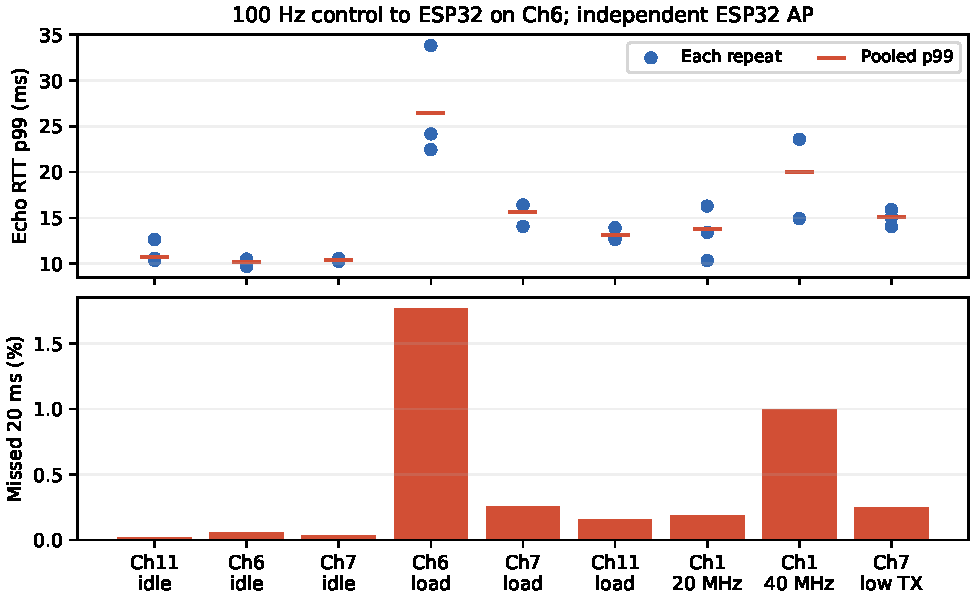
\includegraphics[width=\linewidth]{../experiments/figures/robotics/interference.pdf}\caption{操縦側をCh6とESP32-1へ固定し、ESP32-2 APの条件を変更した比較。idleはAP・ビーコンとTCP接続を保ち、アプリの送信を止めた条件。loadはTCP飽和負荷で、等しい実効Mbpsを保証しない。}\end{figure}

Ch11待機の統合p99は\IdlePninetyNine{} ms、Ch6負荷では\SixPninetyNine{} ms、Ch7負荷では\SevenPninetyNine{} ms、Ch11負荷では\ElevenPninetyNine{} msであった。20 ms期限超過率はそれぞれ\IdleDeadline{}\%、\SixDeadline{}\%、\SevenDeadline{}\%、\ElevenDeadline{}\%である。Ch6とCh7の大小関係は各反復のばらつきも確認する必要がある。同一・部分重複のどちらが常に悪いかを、この少数反復だけで一般化しない。各負荷は飽和TCPである。送信アプリの実効速度はCh6 3.62--6.26、Ch7 3.04--8.07、Ch11 8.64--9.83 Mbpsで、無線レートや送信時間が同じではない。遅延差を周波数位置だけの因果効果とはせず、今回の2リンクの運用条件を含む比較として扱う。


\begin{figure}[htbp]\centering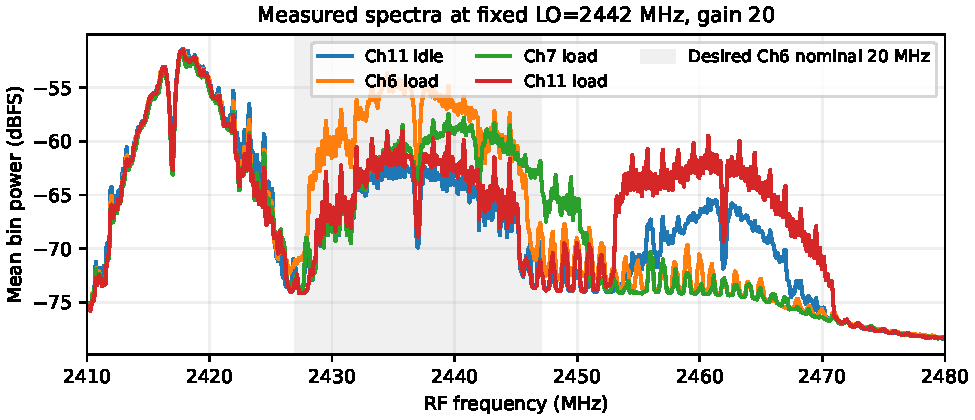
\includegraphics[width=\linewidth]{../experiments/figures/robotics/spectra.pdf}\caption{独立AP比較の実測平均スペクトル。主APはCh6で固定。灰色は主APの名目20 MHz範囲。外来信号と受信機の周波数応答も含む。}\end{figure}
\begin{figure}[htbp]\centering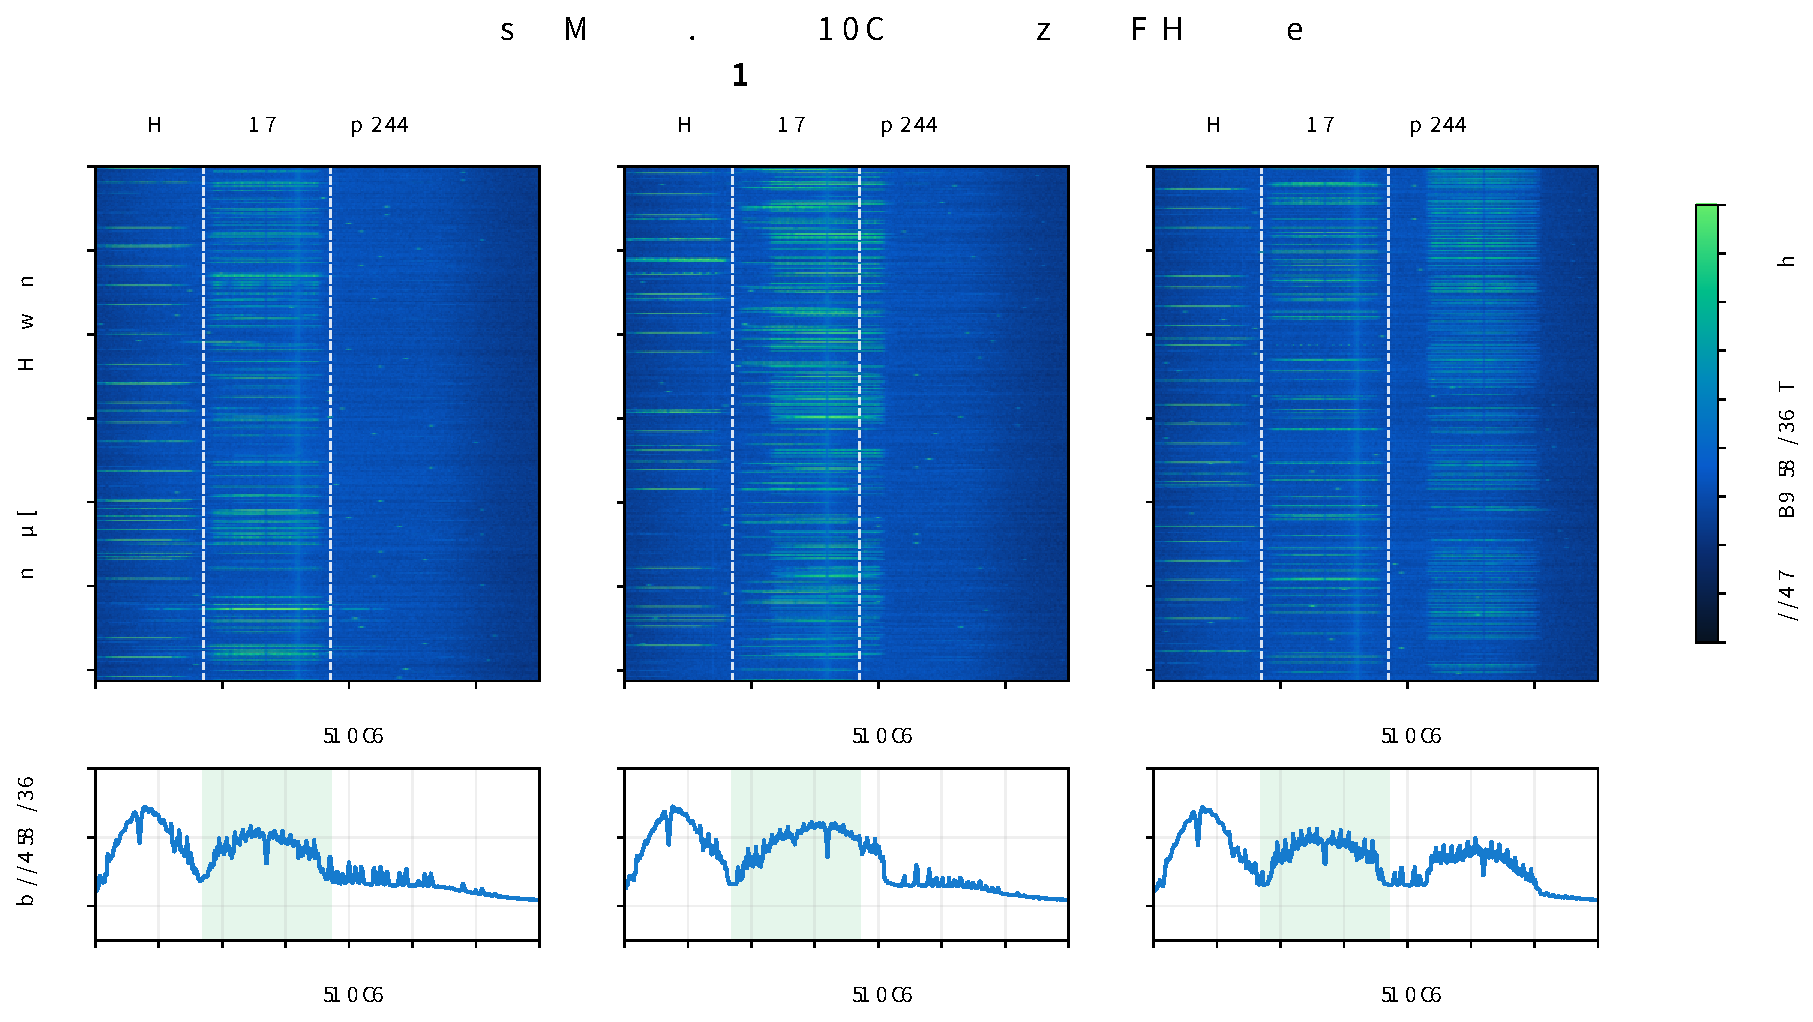
\includegraphics[width=\linewidth]{../experiments/figures/robotics/robotics-blue-green.pdf}\caption{青〜緑の実測ウォーターフォール。画像は各条件の1反復目、RTT注記は3反復の統合値。全パネルで同じ色尺度を使用し、白点線は操縦Ch6の名目範囲。2418 MHz付近の強い成分など外来信号も含み、色を試験APだけに帰属しない。各行は約205 $\mu$sの間欠取得であり、連続占有時間ではない。}\end{figure}

同一チャネルでは、互いを認識できるWi-Fi機器が送信機会を分け合う。部分重複チャネルは名目上の中心周波数が違っても周波数範囲が重なり、受信を妨げたり送信待ちを増やしたりし得る\cite{ciscoRF}。本実験の遅延とスペクトルだけでは、キャリアセンス、隠れ端末、再送、受信機のブロッキングを特定できない。チャネル番号が違うことを独立した帯域と同一視しない、という設計上の判断につながる。

\section{20/40 MHz幅と送信電力設定}
\begin{figure}[htbp]\centering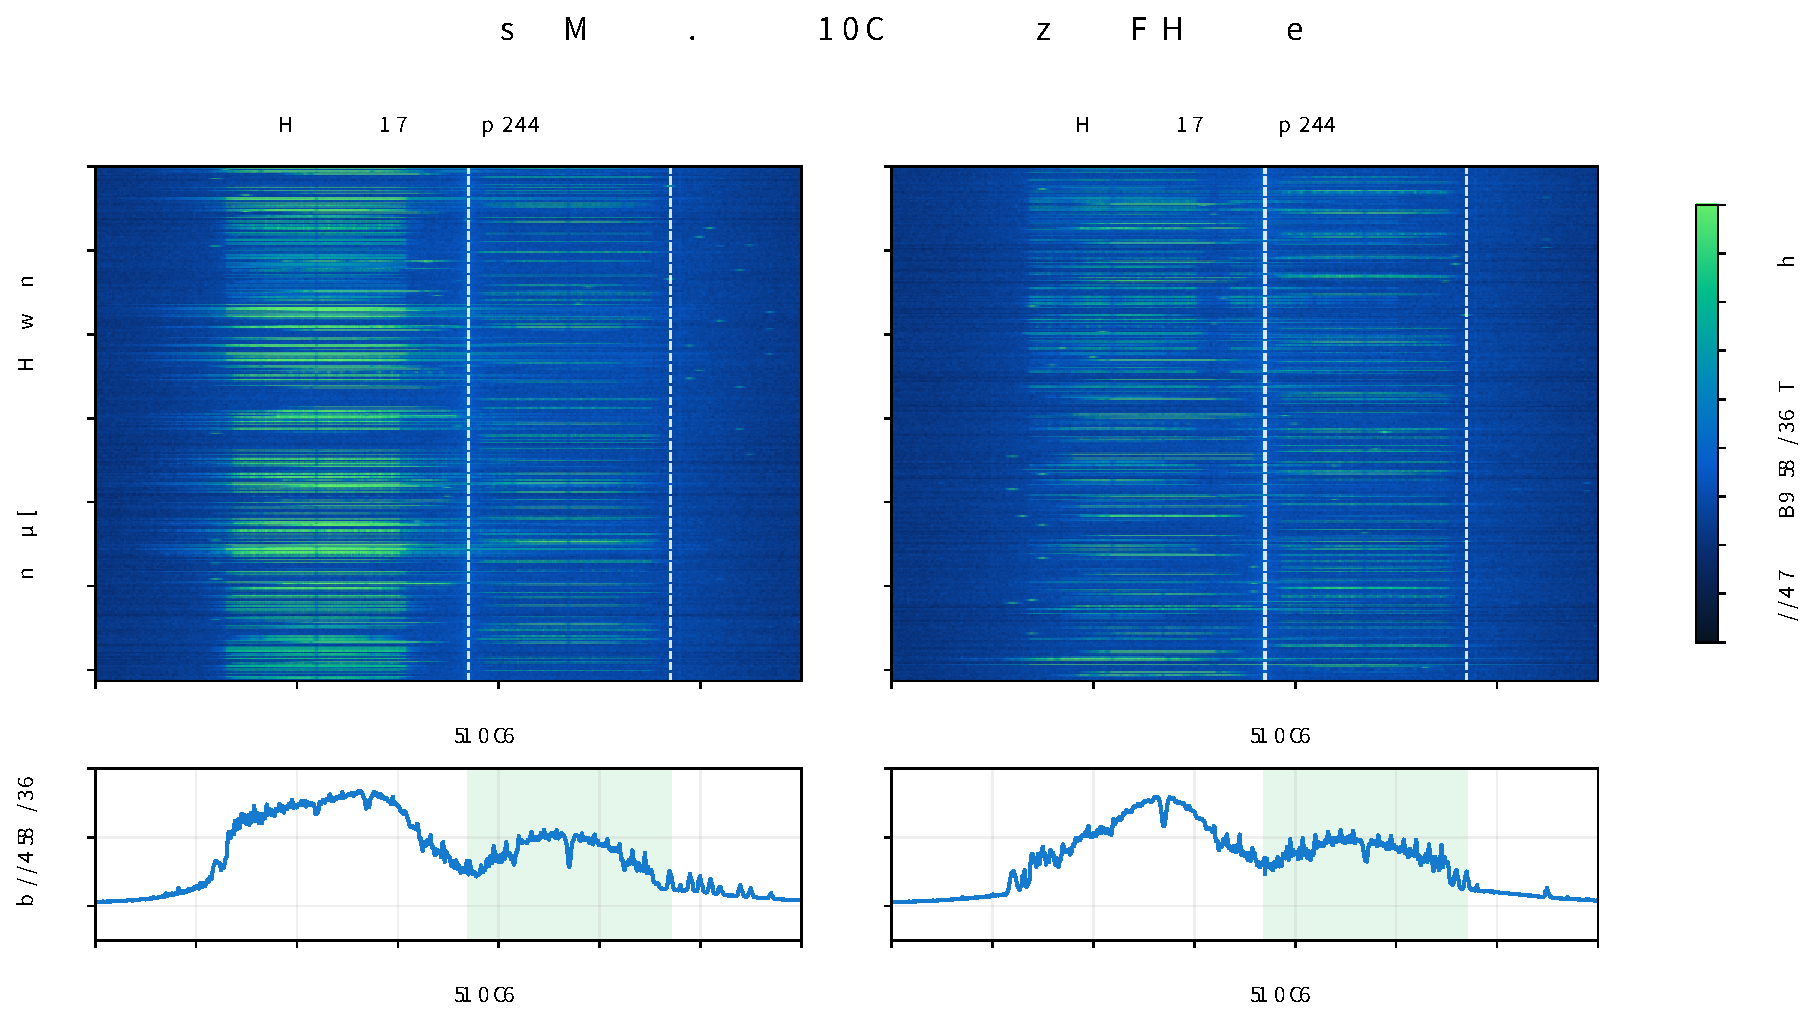
\includegraphics[width=\linewidth]{../experiments/figures/robotics/robotics-width-blue-green.pdf}\caption{Ch1の20/40 MHz設定比較。同じ色尺度・LO=2427 MHz・ゲイン20で観察した。40 MHzの接続幅は3反復ともクライアントのiwログで確認した。広い接続設定でも、全送信が40 MHz波形になるわけではなく、平均スペクトルを理想的な矩形に読み替えない。}\end{figure}
Ch1 HT20時の主リンクp99は\WidthTwentyPninetyNine{} ms、HT40時は\WidthFortyPninetyNine{} ms、20 ms期限超過率は\WidthTwentyDeadline{}\%と\WidthFortyDeadline{}\%だった。副チャネル追加とクライアントの実接続幅は保存したAP状態とクライアントログで確認する。p99の反復範囲には重なりがあり、幅の変更による遅延増加を一律には主張しない。送信アプリ実効速度はHT20 2.68--9.75、HT40 5.27--6.28 Mbpsである。広い帯域の通信が高速化すれば単位データの送信時間が短くなる可能性もあり、重複範囲の拡大だけで結果は決まらない。


名目範囲で考えると、Ch1のHT20は2412 MHz中心、約2402--2422 MHzとなり、Ch6の約2427--2447 MHzと分離する。Ch1+Ch5のHT40は中心が2422 MHzへ移り、約2402--2442 MHzとなるためCh6へ重なる。実際のスペクトルは矩形ではなく、名目範囲の外にも成分がある。帯域幅を広げれば1回の送信で運べる情報を増やせる一方、独立に配置できる通信リンクの数と周波数余裕を減らす\cite{ciscoRF}。今回の幅比較は\textbf{別APの幅を変えた時の操縦通信への影響}であり、操縦AP自身の20/40 MHzの速度比較ではない。先行5 GHzの80 MHz観測も、幅を切り替えた操縦性能比較ではない。

送信電力設定を変えたCh7比較は同じ位置で行った。APの最大電力設定読み返しは通常13.5 dBm、低電力1 dBmであった。主リンクのp99は通常\SevenPninetyNine{} msから低電力\LowPowerPninetyNine{} ms、20 ms期限超過率は\SevenDeadline{}\%から\LowPowerDeadline{}\%となった。低電力時の送信アプリ実効速度は2.23--5.72 Mbpsだった。
 設定値と実際のEIRPやC5入力電力は同一ではない。飽和TCPの実効速度や無線レートも変わり得るので、電力だけを独立変数とする校正済み試験ではない。主リンクを強くすれば全て改善するという結論も、この試験からは導けない。

\section{追加UDP負荷の要求量・受付量・到着量}
TCPは混雑時に転送量自体が変わるため、同じアプリ要求20 MbpsのUDPでも6条件を各3反復比較した。ESP32-2へ1,400 byteのUDP送信を要求し、同じ操縦主リンクを保持した。送信APIの受付パケット数と、ラップトップ2へ到着した識別子・連番を保存した。負荷条件の変更前にAP接続と受信器のready応答を確認した。20 Mbps指定は20 Mbps達成や等しい空中時間を保証しない。
\par
\begin{table}[htbp]\centering\small\caption{UDP負荷比較。主リンクの応答と、別リンクの送信API受付・受信アプリ到着を別々に集計。各3反復。受付/到着Mbpsは負荷全区間の範囲で、PHY速度ではない。}\begin{tabular}{lrrrrrr}\toprule 条件 & p99 ms & 20 ms超過\% & 欠落\% & 受付Mbps & 到着Mbps & 別リンク未到着\%\\\midrule
Ch11idle & 13.7 & 0.08 & 0.00 & 0.00--0.00 & 0.00--0.00 & --\\
Ch6 & 19.4 & 0.82 & 0.00 & 5.23--8.12 & 5.19--8.10 & 0.2--0.7\\
Ch7 & 18.3 & 0.56 & 0.00 & 2.90--7.61 & 2.86--7.55 & 0.7--1.4\\
Ch11 & 58.4 & 5.64 & 0.01 & 1.19--6.52 & 1.13--6.50 & 0.3--4.3\\
Ch1w20 & 16.1 & 0.24 & 0.00 & 3.56--7.65 & 3.56--7.62 & 0.1--0.3\\
Ch1w40 & 133.9 & 40.59 & 0.00 & 0.35--5.07 & 0.31--5.06 & 0.2--10.3\\
\bottomrule\end{tabular}\end{table}
\par

この未到着率は送信APIで受付済みの連番が受信アプリへ届かなかった割合であり、Wi-FiのPHYパケット損失率ではない。端末・OS・収集器の影響も含む。送信APIで受け付けられる量自体が小さい場合、要求値で通信量を統制できたとは扱わない。
主リンクp99の各反復範囲はCh6 16.7--21.2、Ch7 17.0--19.0、Ch11 24.3--79.4 msだった。TCP比較だけの順位や代表値をUDPへ外挿しない。分離チャネルでも遅い応答が観測された場合には、周波数分離だけで主リンクが無影響と決めず、実通信量・負荷波形・端末処理を合わせて確認する。現在の測定だけで再送、受信ブロッキング、外来通信、バッファリングのどれかへ帰属することはできない。
\par
\begin{figure}[htbp]\centering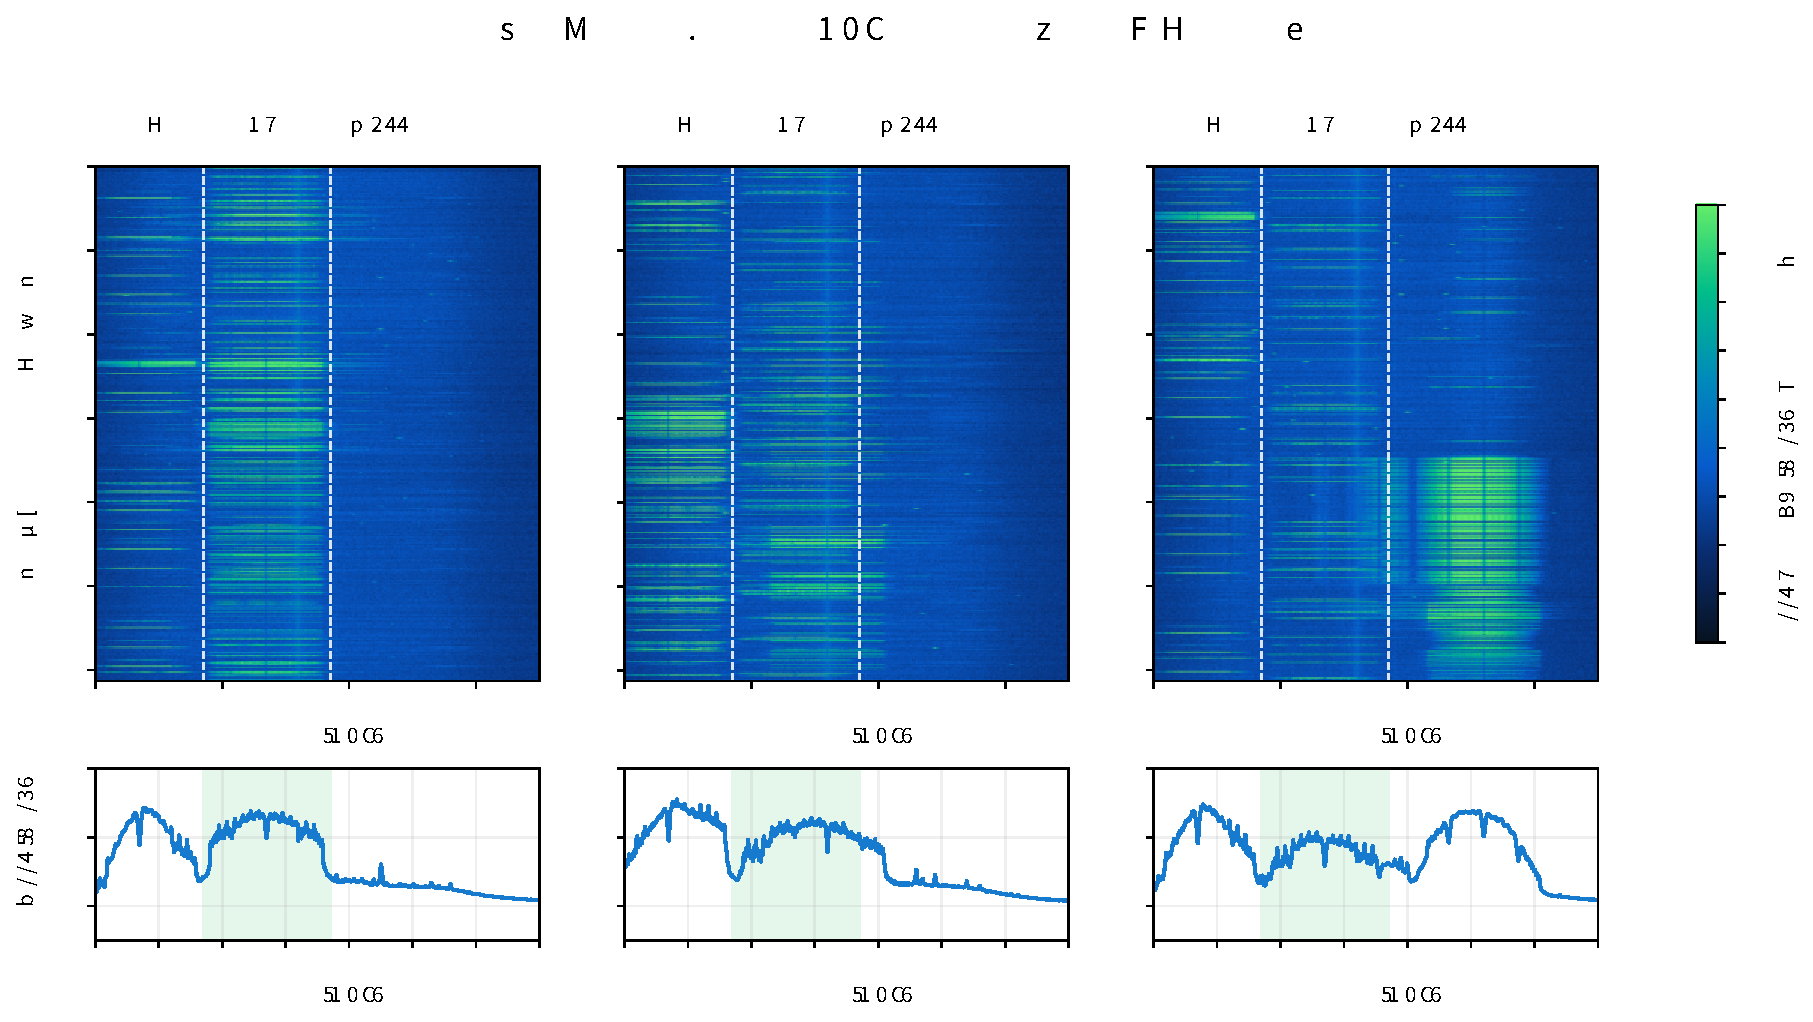
\includegraphics[width=\linewidth]{../experiments/figures/robotics/robotics-udp-blue-green.pdf}\caption{追加UDP要求20 Mbps条件の1反復目。色尺度はTCP画像と同じ。要求値と実通信量が一致しないため、画面注記は実測受付量を使う。}\end{figure}

\section{受信端末の基準遅延とRF干渉}
初期構成ではラップトップ2をUDP反射端末にしたが、別AP負荷なしでもp99約116 msが出た。2/20 Mbpsの下りTCP、省電力onからoffへの再適用、mt76のruntime-pmとdeep-sleepの一時無効化でも約109--116 msの裾が残った。設定は元に戻した。mt76の2つの設定はドライバが別々に公開する制御である\cite{mt76debug}が、本結果はそれらを遅延原因と特定するものではない。

この遅延を干渉の効果に加算することを避け、全主比較の操縦相手をESP32-1へ統一した。端末・APのバッファリングや無線送受信のどの区間が原因かは未確定である。初期構成2試行と端末診断の短時間試行は予備データとして保持し、主比較には含めない。負荷停止の実装競合と自律クライアントの切断判定も修正し、原ログを残した。

\section{C5による観測範囲と評価の限界}
本追加実験は\Conditions{}試行、\ControlPackets{}操縦UDP、\Snapshots{} I/Qスナップショットを主比較へ保存した。主比較の最大I/Qレール到達率は\RailMax{}\%である。名目RF観測時間比は約\DutyRatio{}\%であり、ほとんどの時間を直接観測していない。先行115条件・27,540取得の受信系評価で確認したLO端部の減衰、ゲインによる飽和、固定周期による位相偏りは今回も解釈上の制約となる。

SDRは周波数位置と広がり、強いバーストが増えることを可視化する。一方、指令が期限に間に合うかはUDP時刻列で測る必要がある。今回も色の変化をパケット欠落数や帯域占有率へ直接換算しない。RTT、TCP実効速度、I/Qを条件単位で併記することで、電波の見た目だけから通信性能を推測する誤りを減らせる。

室内の外来通信、位置・向き、送信機のアンテナと無線レート、少数反復、試験順序に制約がある。同じ実効負荷・既知入力電力・同じPHYレートにそろえた比較ではない。距離掃引、隠れ端末配置、操縦AP自身の幅変更、優先度制御、実機の制御誤差と停止判断は今後の候補となる。ロボコン会場へ数値をそのまま外挿せず、同じ評価指標で会場配置を試す価値を示す実験である。


\clearpage\section*{先行観測：SDR画像を読むための補足}
\graphicspath{{../experiments/figures/baseline/}}
\section{目的と実験環境}
基礎実験と追加評価を通じた目的は、Wi-Fiのチャネル変更や通信負荷がスペクトル上でどう現れるかを観察し、SDRの表示と実際の観測能力を区別することである。通常の室内で実施し、電波暗室、校正信号源、距離の実測は用いていない。他のAPや端末も存在するため、観測信号をすべて実験APに帰属させることはできない。

観測PCはUbuntu 22.04.5、カーネル6.18.6-1-liquorix-amd64、NetworkManager 1.36.6、Intel BE200（iwlwifi）を使用した。C5はUSB Serial/JTAG経由で接続した。ESP-SDR\cite{sdr}は固定したESP-IDFコミット\texttt{25fe69f946311abdaf9ad56591f25fedbc20ac98}でビルドし、起動時の2.4 GHz帯選択を明示する局所修正を加えた。

\begin{figure}[htbp]\centering
\begin{tikzpicture}[box/.style={draw,rounded corners,align=center,font=\small,minimum width=34mm,minimum height=12mm},>=Latex]
\node[box] (router) {既存ルーター\\インターネット};
\node[box,right=13mm of router] (laptopOne) {ラップトップ1（Intel AX210）\\Wi-Fi上流・NAT};
\node[box,right=13mm of laptopOne] (local) {観測PC\\BE200 Soft AP};
\node[box,below=17mm of local] (client) {ラップトップ2（MT7921E）\\TCP受信クライアント};
\node[box,below=17mm of laptopOne] (c5) {ESP32-C5\\I/Q受信};
\draw[->] (router)--node[above,font=\scriptsize]{Wi-Fi} (laptopOne);
\draw[->] (laptopOne)--node[above,font=\scriptsize]{Ethernet} (local);
\draw[<->] (local)--node[right,font=\scriptsize]{2.4 GHz} (client);
\draw[<->] (c5)--node[above,sloped,font=\scriptsize]{USB} (local);
\end{tikzpicture}
\caption{実験構成。制御はTailscale SSH、負荷のTCPデータは実験APのローカルIP宛てに送る。C5は周囲の信号も受信する。}\end{figure}

ラップトップ1のEthernetをIPv4 shared（192.168.58.10/24）とし、観測PCを192.168.58.11、デフォルトゲートウェイとDNSをラップトップ1に設定した。観測PCの無線を停止してもEthernetに固定したHTTPSアクセスが成功することを確認した。実験APのサブネットは10.78.0.0/24、WPA2、DHCPである。実験用NAT/FORWARDチェーンは固有名で作成し、終了時に削除した。元の接続プロファイルは保存した。IntelのAP/masterモードには公式なサポート制限がある\cite{intel,iwl}ため、能力広告だけで動作可と判断せず、hostapdと\texttt{iw}の結果を記録した。

\section{測定・解析方法}
\subsection{I/Q取得とデータ保全}
\texttt{CAP16}で1回16,380組の符号付き8 bit I/Qを取得する。コマンド名の16は保存データが16 bit/成分であることを意味しない。サンプル数とCRC32を検証してからNPZへ保存し、設定、UTC時刻、ホスト単調時計、取得時間、通信実績、AP状態をJSONに記録した。USBは2 Mbaudで使用した。終了時にシリアル端末設定のVMIN=1、VTIME=0を復元した。VMIN=0が残るとChromeが読み取り0 byteを切断と解釈する問題を実機で確認した。

\subsection{スペクトル推定と単位}
$x[n]=(I[n]+jQ[n])/128$とし、各FFT区間の複素平均を除去した後Hann窓$w[n]$を適用する。
\begin{equation}
P[k]=\frac{\left|\sum_{n=0}^{N-1}(x[n]-\bar x)w[n]e^{-j2\pi kn/N}\right|^2}{(\sum_{n=0}^{N-1}w[n])^2}.
\end{equation}
スナップショット内の区間電力を線形平均し、平均スペクトルも線形平均後に$10\log_{10}$を取る。最大値曲線はスナップショット電力のビン別最大値である。C5の符号規約に従い$f_{\mathrm{RF}}=f_{\mathrm{LO}}-f_{\mathrm{baseband}}$とした。通常のFFT長は2,048、80 MS/sでのビン間隔は39.0625 kHz、Hann窓の等価雑音帯域は約58.6 kHzである。解析コードの周波数軸と規格化は人工的な複素トーンでも確認したが、実験図には人工トーンを含めていない。

図のdBFSはこの規格化による相対ビン電力であり、dBmや電界強度への校正値ではない。複素フルスケールの定義にも依存する。ゲイン、アナログフィルター、FFT長を変えた結果を、送信電力の変化とそのまま同一視しない。

\subsection{間欠取得と比較指標}
80 MS/sで16,380サンプルの名目時間は204.75 $\mu$sである。USB転送・処理中は連続RF観測ではなく、ウォーターフォールの縦軸を取得番号で表示する。名目取得時間の合計とホスト経過時間の比
\begin{equation}R=\frac{M\,16380/f_s}{t_{\mathrm{end}}-t_{\mathrm{start}}}\end{equation}
はイベント捕捉率ではない。ファームウェア報告時間にも内部処理を含むため、$16380/f_s$とは区別する。

固定ゲイン20の比較に限り、DC除去後のスナップショットRMSが$-40$ dBFSを超える割合を補助指標とした。これは便宜的なしきい値であり、チャネル占有率やWi-Fiフレーム復号結果ではない。飽和指標はI/Q成分が$-128$または127に一致した割合である。

\section{2.4 GHzのチャネルと通信負荷}
APを20 MHzに設定し、1・6・11チャネル（2412・2437・2462 MHz）で待機時と要求20 MbpsのTCPダウンリンクを各2回測定した。各中心周波数で180回、共通LO=2440 MHzで負荷時120回取得した。要求通信は18秒、取得開始は通信開始から約2秒後である。各測定で実際の受信速度を保存した。主比較のゲインは20、アナログ帯域は自動である。
保存データは51条件、合計9,140スナップショットである（探索測定を含む）。
探索測定の負荷生成失敗3条件は主要比較から除外した。保存した全I/QのCRCを再検証して一致を確認した。

\begin{table}[htbp]\centering
\caption{固定ゲイン20、RMSしきい値$-40$ dBFSを超える取得割合。占有率ではない。}
\begin{tabular}{rrrrrr}
\toprule
Ch & 反復 & 待機(\%) & 負荷(\%) & 実効Mbps & 飽和(\%)\\\midrule
1 & 1 & 4.4 & 21.7 & 19.99 & 0.0000\\
1 & 2 & 6.1 & 37.8 & 19.17 & 0.0000\\
6 & 1 & 4.4 & 34.4 & 19.88 & 0.0000\\
6 & 2 & 4.4 & 41.7 & 19.81 & 0.0000\\
11 & 1 & 3.9 & 23.9 & 19.99 & 0.0000\\
11 & 2 & 1.1 & 23.9 & 19.99 & 0.0000\\
\bottomrule\end{tabular}\end{table}

待機時のしきい値超過割合1.1--6.1\%に対し、負荷時は21.7--41.7\%であった。主要比較のレール到達割合は0\%である。
\plot{channels}{.95}{共通LO=2440 MHzでの最大スナップショット電力。設定チャネルに対応する信号位置が変化する。AP停止時にも外来信号がある。受信アナログ帯域の上限48 MHzにより80 MHz表示の端は同じ感度とは限らない。}
\plot{channel-waterfalls}{1}{チャネルごとの実測ウォーターフォール。破線は設定中心周波数。縦方向の隙間は未観測RF時間を表さず、取得番号を表す。}
\plot{idle-loaded}{.95}{6チャネルの待機・負荷条件、各2回。少数の強い信号が線形平均へ寄与する。}
\section{受信設定と表示の違い}
\subsection{サンプルレートとFFT長}
80・40・20 MS/sを比較した。サンプルレートは表示できる周波数範囲と1取得の名目RF時間を変える。20 MS/sでは20 MHzチャネルの端に余裕がなく、フィルターやエイリアシングの影響を含めて評価する必要がある。同一データを256・512・1024・2048点で再解析するとビン間隔は312.5・156.25・78.125・39.0625 kHzとなる。FFT長によるビン電力のノイズ床低下は、受信機の物理的な雑音が減った証拠ではない。
\plot{sample-rates}{.9}{サンプルレート比較。同じ通信要求でも観測範囲とビン幅が変わる。}
\begin{table}[htbp]\centering
\caption{サンプルレートごとの取得速度と時間比。報告取得時間は処理時間を含む。}
\begin{tabular}{rrrr}
\toprule
MS/s & 取得/s & 名目時間比(\%) & 報告時間($\mu$s)\\\midrule
80 & 19.78 & 0.405 & 1881\\
40 & 19.71 & 0.807 & 2087\\
20 & 19.82 & 1.623 & 2494\\
\bottomrule\end{tabular}\end{table}

\plot{capture-gaps}{.9}{取得速度と名目サンプル時間比。全イベントを連続受信していると解釈しない。}
\plot{fft-comparison}{.95}{同一生データのFFT長比較。ビン電力の規格化は同じだが、各ビンの帯域が異なる。}
\subsection{アナログフィルターとゲイン}
帯域要求11・20・40・48 MHzを比較した。狭い帯域は帯域外の成分を抑える一方、Wi-Fiチャネル内の端も減衰し得る。ゲイン20・40・60とHardware AGCを比較した。高ゲインではレール到達とスペクトルの歪みを確認する。最初のゲイン40の探索測定は保存したが、クリッピングを認めたため主要なチャネル比較をゲイン20で取り直した。
\plot{filters}{.9}{受信アナログ帯域の比較。表示スパンとアナログ通過帯域を区別する。}
\begin{table}[htbp]\centering
\caption{ゲイン設定と取得電力、飽和。RMSはDC除去後。}
\begin{tabular}{lrrr}
\toprule
ゲイン & RMS中央値 & RMS95百分位 & 飽和(\%)\\\midrule
MANUAL20 & -50.54 & -24.74 & 0.0000\\
MANUAL40 & -41.94 & -4.40 & 0.3397\\
MANUAL60 & -35.35 & 1.93 & 12.7318\\
HARDWARE & -17.79 & -8.84 & 0.0340\\
\bottomrule\end{tabular}\end{table}

\plot{gain}{.9}{受信ゲインの比較。高い表示電力は受信感度や測定精度の改善を必ずしも意味しない。}
\begin{table}[htbp]\centering
\caption{6チャネルでの要求速度と実効速度、しきい値超過割合。}
\begin{tabular}{rrr}
\toprule
要求Mbps & 実効Mbps & 超過割合(\%)\\\midrule
2 & 2.00 & 5.6\\
20 & 19.84 & 39.4\\
60 & 46.53 & 52.8\\
\bottomrule\end{tabular}\end{table}

\plot{traffic}{.9}{要求TCP速度2・20・60 Mbpsと待機条件。実効速度は結果表を参照。}
\section{ビーコンとAPチャネル幅}
ビーコン間隔50・100・500 TUを比較した。1 TUは1.024 ms\cite{hostap}であり、設定値は51.2・102.4・512 msに相当する。待機時でもビーコン、管理フレーム、クライアントのバックグラウンド通信、外来信号がある。スナップショットが短く間欠的であるため、図から全ビーコン数や正確な周期を推定することはできない。

\plot{beacons}{1}{成功したビーコン設定の比較。短い取得と異なる取得回数のため、図の横縞の数だけで周期を比較しない。}

40 MHz要求ではhostapdのHT40+設定を用い、\texttt{iw}が報告する実際の帯域と共存処理のログを確認した。今回の実際の帯域は20 MHzであり、40 MHz送信の成功例とは扱わない。ログには重複する20 MHz HT BSSの検出があり、共存処理との関連が示唆される。要求帯域だけを成功判定には用いない。
\plot{ap-width}{.9}{20 MHz設定と40 MHz要求の比較。LOが異なるため、受信周波数応答の影響も含む。実際の帯域は結果表で確認する。}
\section{既存5 GHz APの受信観測}
別実験ではラップトップ2を既存ルーターに戻し、primary48チャネル、80 MHz幅、center5210 MHzを\texttt{iw}で確認してC5を5210 MHzへ設定した。待機・要求20 Mbpsを各2回測定した。通信はTailscale経由であり、ラップトップ1とラップトップ2の両方が同じ既存ルーターを通るため、信号増加を単一送信機に帰属させない。受信アナログ帯域上限48 MHzでは80 MHzチャネル全体を一度に均一感度で測定できない。
負荷時のレール到達割合は約0.51--0.55\%であり、強い信号の電力比較には飽和の影響がある。この飽和に対し、後述する分割取得ではゲイン20へ下げて再評価した。
\begin{table}[htbp]\centering
\caption{既存5 GHzルーター観測。ゲイン40、中心5210 MHz。}
\begin{tabular}{lrrrrr}
\toprule
条件 & 反復 & 実効Mbps & RMS中央値 & RMS95百分位 & 飽和(\%)\\\midrule
idle & 1 & - & -45.46 & -12.01 & 0.0472\\
load20 & 1 & 19.88 & -45.07 & -3.08 & 0.5474\\
idle & 2 & - & -45.33 & -10.67 & 0.0756\\
load20 & 2 & 19.88 & -45.07 & -3.34 & 0.5124\\
\bottomrule\end{tabular}\end{table}

\IfFileExists{../experiments/figures/baseline/router5g.pdf}{\plot{router5g}{.95}{既存5 GHzルーターを用いた受信観測。BE200が5 GHz APとして動作した結果ではない。}}{}


\section{追加評価への展開と保存条件}
基礎観察で残った帯域・飽和・間欠取得の問題を、時刻計測、LO掃引、設定電力比較、無作為取得、BLE共存および5 GHz分割取得で掘り下げた。Intelの実際の動作モジュールはiwlmldであり、ラップトップ2はMT7921E（mt7921e）を使用した。主要な追加比較は手動ゲイン指数20・80 MS/sで実施した。基礎実験の負荷生成失敗3条件と追加実験のスリープ影響が疑われる初回50 TUの2条件は、原データを保持して主要比較から除外した。条件数は校正された独立反復数ではない。

追加データもローカルの生I/Q・JSON・主要PCAPと、ラップトップ2の全PCAP原本へ保存した。取得区間に装置時刻を加え、固定・乱数標本化とLO条件の順序変更を実施した。十分な無作為化反復や外来信号の除去を保証するものではない。
\graphicspath{{../experiments/figures/receiver/}}
\section{時刻計測とPCAPの解釈}
\subsection{取得時刻を追加したファームウェア}
診断ビルドに\texttt{CLOCK?}と\texttt{CAPTIME?}を追加した。前者は\texttt{esp\_timer\_get\_time()}、後者はベンダー取得関数の呼出し直前・直後の装置時刻を返す。従来の\texttt{CAP16}応答形式は維持した。時計問い合わせを各条件の前後32回実行し、往復が短い各8回から装置時刻とホスト単調時計の一次換算を求める。半往復時間と換算残差を誤差幅として保存する。

この時刻は正確なADC開始トリガではない。RF取得は不透明なベンダー関数の実行区間のどこかで行われる。CRCや取得成功の確認も、連続RF観測を保証しない。80 MS/sのサンプル時間は
\begin{equation}T_s=16380/(80\times10^6)=204.75\ \mu\mathrm{s}\end{equation}
であるが、実行区間は約1.88 ms、時計換算の幅は約$\pm0.6$ ms、取得間隔は約49 msである。
\plot{timing-audit}{.95}{別々の意味を持つ4種類の時間。対数軸。処理区間と名目RF時間を同一視しない。}

\subsection{PCAPの観測範囲と関連表}
BE200にAPとモニターを併用し、ラップトップ2にも管理接続とモニターを併用した。Linux Wirelessの資料はモニター併用をbest effortとする\cite{modes}。BE200側には自局ビーコンが現れず、送信通知と受信フレームが混在した。PCAPはスナップ長128 byteとし、復号したアプリケーション内容は解析しない。RadiotapのTSFTは受信MAC時刻であり\cite{tsft}、PCAPレコードのホスト受渡し時刻とは異なる。受信時刻フィールドの存在も記録した\cite{timestamp}。ラップトップ2側の別PCAPから実験APのビーコン5,721件を抽出し、ビーコン本文の50・100・500 TUをそれぞれ1,251・4,399・71件確認した。欠落とスリープ期間があるため、これらの件数をAPの全送信数とはしない。

ホストPCAP時刻がC5取得関数の区間と換算誤差幅に入るかを集計した。さらに追加幅$\pm0,1,5,20$ msと、送信通知を含む場合・受信のみの場合を保存した。しきい値はDC除去後の全帯域スナップショットRMS $>-40$ dBFSである。表の「関連・検出」は真陽性とは限らない。パケットのRF送信時間、観測漏れ、他送信機、USB時刻誤差を含むためである。
\begin{table}[htbp]\centering\small
\caption{同時刻窓との関連集計。真陽性・真陰性を保証する表ではない。}
\begin{tabular}{lrrrrr}
\toprule
条件 & 追加$\pm$ms & 関連・検出 & 関連・無検出 & 無関連・検出 & 無関連・無検出\\\midrule
idle & 0 & 0 & 7 & 54 & 939\\
idle & 5 & 2 & 16 & 52 & 930\\
idle & 20 & 5 & 54 & 49 & 892\\
load20 & 0 & 185 & 367 & 207 & 241\\
load20 & 5 & 392 & 608 & 0 & 0\\
load20 & 20 & 392 & 608 & 0 & 0\\
\bottomrule\end{tabular}\end{table}

\plot{pcap-association}{.95}{時間窓を広げるだけでも関連表が変化する。送信通知を含む集計。ラベルを確定した検出器の混同行列ではない。}

\subsection{PC間時計差の変化}
ラップトップ2に一時的なTCP時計応答を用意し、時刻問い合わせ80回中の最短往復を採用した。最初の時計差は数msであったが、復帰後は約0.56秒の差を観測した。時刻差の変化を記録しており、変化の内部原因までは確定していない。前後で一定の時計差を仮定して、ラップトップ2の全PCAPへ一律のオフセットを加える方法は採用しない。既存のPC間絶対時刻だけではパケット単位の真値を構成できない。
\plot{../experiments/figures/overview/peer-clock-offset}{.9}{測定したPC間時計差。誤差棒は半往復時間であり、スリープをまたぐ時計変化の上限ではない。}

\section{固定周期とランダム標本化}
ビーコン50・100・500 TU（51.2・102.4・512 ms）に対し、平均取得間隔を102.4 msに設定した。固定取得は絶対予定時刻へ待ち、ランダム取得は各間隔を65--139.8 msの一様乱数とした。種を記録し、各500回取得した。固定・ランダムの実行順を100 TU条件で逆転した。これは十分な無作為化反復の代替ではない。

位相を$\phi_i=(t_i-t_0)\bmod T$とし、集中度を
\begin{equation}R_h=\left|\frac1M\sum_i e^{j2\pi h\phi_i/T}\right|\end{equation}
で評価した。ここで$t_i$は装置側取得開始、$t_0$は任意の原点であり、ビーコンのRF先頭ではない。100 TU固定では同じ位相、500 TU固定では5つの位相へ集中する。5位相の分布は$R_1$だけでは一様分布と区別しにくいため、$R_5$も併記する。
\begin{table}[htbp]\centering\small
\caption{取得位相の集中度と信号しきい値。位相原点は最初の取得開始。}
\begin{tabular}{rlrrrrrr}
\toprule
TU & 周期 & 間隔ms & 標準偏差ms & $R_1$ & $R_5$ & RMS超過\% & 帯域超過\%\\\midrule
50 & fixed & 102.401 & 0.494 & 0.999 & 0.980 & 7.4 & 3.2\\
50 & random & 102.116 & 21.732 & 0.039 & 0.007 & 11.4 & 3.4\\
100 & fixed & 102.401 & 0.490 & 1.000 & 0.995 & 6.6 & 2.2\\
100 & random & 103.303 & 21.344 & 0.059 & 0.013 & 8.8 & 2.6\\
500 & fixed & 102.401 & 0.490 & 0.000 & 1.000 & 2.6 & 1.8\\
500 & random & 102.862 & 21.023 & 0.003 & 0.038 & 5.2 & 0.6\\
\bottomrule\end{tabular}\end{table}

\plot{sampling-phase}{1}{名目ビーコン周期に対する取得位相。原点は各条件の最初の取得。絶対的なビーコン到着位相やパケット捕捉率の図ではない。}

独立・一様位相で周期$T$のイベントを観測し、イベント継続時間を$T_e$とすると、理想的な時間重なり確率は
\begin{equation}p_{\mathrm{overlap}}=\min(1,(T_s+T_e)/T)\end{equation}
であり、$T_s/T$だけではイベント自身の長さを無視する。実際にはしきい値、周波数帯域、外来信号と時間分解能がある。全帯域RMSに加え2433--2441 MHzのビン電力和 $>-45$ dBFSも集計したが、いずれもビーコンを復号・同定した結果ではない。周期設定にロックすると偏った位相を繰り返し見ることを実測できた一方、真のビーコン検出率の定量確定には、ADCトリガ時刻か十分な時刻同期が必要である。

\section{LO掃引による有効周波数応答}
APは6チャネルに固定し、LOを2407--2467 MHzで10 MHz刻みに変更した。帯域要求48 MHz、ゲイン指数20、要求TCP 20 Mbps、各150回、2反復、反復ごとに順序を変更した。同じRF帯域2433--2441 MHzの電力和を用い、2437 MHzのDC近傍$\pm0.15$ MHzをすべての条件で除外する。平均と90百分位を分け、通信の間欠性による交絡を示す。FFTはHann窓2048点、窓和の二乗で規格化し、線形平均してから対数にする。

LO中央の90百分位を0 dBとした有効応答を表に示す。単一既知キャリアの伝達関数ではなく、8 MHz帯域にわたるWi-Fiの平均的な応答である。RF源の時間変化、フィルター、LO位置、受信機の校正状態を含む。中心から$\pm30$ MHzでは約9--10 dB低下し、80 MHz表示の両端を均一感度として扱えないことを確認した。
\begin{table}[htbp]\centering\small
\caption{2433--2441 MHzの固定RF帯域を用いた有効応答。90百分位、中央条件基準。}
\begin{tabular}{rrrr}
\toprule
LO MHz & RF中心$-$LO MHz & 反復1 dB & 反復2 dB\\\midrule
2407 & 30 & -9.96 & -9.90\\
2417 & 20 & -1.57 & -1.74\\
2427 & 10 & -0.61 & -0.33\\
2437 & 0 & 0.00 & 0.00\\
2447 & -10 & -0.27 & -0.33\\
2457 & -20 & 1.14 & -1.21\\
2467 & -30 & -9.05 & -9.85\\
\bottomrule\end{tabular}\end{table}

\plot{lo-response}{1}{固定RF帯域の有効応答。各反復の中央LO条件を基準とする。縦軸は校正されたフロントエンド利得ではない。}
\plot{lo-spectra}{.95}{同一RFチャネルのスペクトルをLO位置を変えて観測。灰色部分が比較用の固定RF帯域。}

さらに帯域要求11・20 MHzについてLO=2417・2437・2457 MHzを取得した。狭いアナログ通過帯域と広い表示スパンを区別し、フィルター内外での信号減衰を比較できる。LO変更ごとの生データと条件は保存した。\maybeplot{filter-response}{.95}{11・20・48 MHz帯域要求での固定RF帯域応答。48 MHzのみ2反復で、反復1を表示。各帯域の中央LO条件で規格化した。}

\section{送信電力設定によるレベル応答}
ステップアッテネータがないため、AP送信電力を5・10・15・20 dBmへ要求し、\texttt{iw}の報告値を記録した。ゲイン指数20・40、各150回、2反復、要求TCP 20 Mbpsとし、電力条件の順序を変更した。受信対象の位置は意図的には変更していないが、伝搬経路や距離は校正していない。PHYレート変更、通信の時間占有、他信号の影響も含む。
\IfFileExists{full.tex}{\begin{table}[htbp]\centering\small
\caption{送信電力設定の比較、2反復平均。入力校正や感度の測定ではない。}
\begin{tabular}{rrrrrr}
\toprule
ゲイン & 要求dBm & 報告dBm & 帯域P90 dBFS & レール\% & 実効Mbps\\\midrule
20 & 5 & 5.0 & -41.68 & 0.0000 & 19.94\\
20 & 10 & 10.0 & -39.29 & 0.0000 & 19.86\\
20 & 15 & 15.0 & -39.17 & 0.0000 & 19.85\\
20 & 20 & 20.0 & -39.19 & 0.0000 & 19.86\\
40 & 5 & 5.0 & -23.52 & 0.0763 & 19.93\\
40 & 10 & 10.0 & -20.85 & 0.0732 & 19.85\\
40 & 15 & 15.0 & -20.85 & 0.0927 & 19.86\\
40 & 20 & 20.0 & -20.14 & 0.1101 & 19.92\\
\bottomrule\end{tabular}\end{table}
}{}
\maybeplot{txpower-response}{1}{送信電力設定と受信帯域の90百分位・レール到達率。設定dBmをC5入力dBmと置き換えない。}

指数20での帯域90百分位（2反復のdB値平均）は5・10・15・20 dBm設定に対して$-41.68$, $-39.29$, $-39.17$, $-39.19$ dBFSとなり、10 dBm以降はほぼ横ばいだった。単純回帰の傾きは0.148--0.155 dB/dBにとどまり、想定した1 dB/dB応答にはならなかった。指数20のレール到達率はすべて0、指数40では平均0.073--0.110\%となった。実効TCP速度は約19.9 Mbpsを維持した。\texttt{iw}報告値は要求値を追随したが、実放射電力やC5端子の入力を測ったものではない。この非比例性が送信側制御・受信側応答・伝搬・背景信号のどれによるかは分離できない。

この結果から相対応答や飽和を評価できるが、受信機の最小検出電力、絶対ダイナミックレンジ、校正入力に対する1 dB/dBの直線性は決定できない。指数20の測定を主要な応答比較に用い、高ゲインのレール到達は歪みの指標として扱う。簡単な直線近似の係数は\texttt{ota-linearity-fits.json}に保存したが、受信機固有の線形性の保証値ではない。

\section{AGC負荷過渡と訓練系列候補}
\subsection{秒単位の負荷切替}
6秒待機・6秒TCP 20 Mbpsを4回繰り返し、ゲイン指数20とHardware AGCで各1100回取得した。通信の要求開始・終了と実際の受信速度を記録した。強いRF信号の正確な立上りではなく、通信負荷要求の立上りである。約49 ms間隔のスナップショットから、数$\mu$sのAGC追従時間を決めることはできない。
\maybeplot{agc-transient}{1}{全帯域RMSの負荷過渡。橙色はTCPを要求した時間で、各パケットの実際の送信時刻ではない。}

\subsection{OFDM短訓練系列の周期性解析}
80 MS/sの複素I/Qをフィルター付きで20 MS/sへ変換し、16サンプル（0.8 $\mu$s）遅延との64点相関を求めた。正規化相関$>0.92$、電力$>10^{-4}$、相関の連続48点以上、および多周波成分の条件を満たす部分をSTF候補とした。狭帯域の単一キャリアは除外する。候補の相関位相から
\begin{equation}\widehat{\Delta f}_{\mathrm{RF}}=-\frac{\arg\sum z^*[n]z[n+16]}{2\pi(16/(20\times10^6))}\end{equation}
を計算した。実装の符号・尺度は既知35 kHzの人工的な周期多音信号で検証した。図は実際のI/Qの候補だけであり、検証信号を混ぜていない。
\maybeplot{cfo-candidates}{.95}{STF周期性の条件を満たした周波数差候補。送信機のMAC識別、RF基準源、温度計測がないため、C5の絶対周波数精度や温度ドリフトの校正値ではない。}

20 Mbps条件では1,000取得中166個の候補を得た。周波数差の5・50・95百分位は$-30.04,-10.50,-8.95$ kHzであり、約$-30$ kHzと$-10$ kHzの複数群を認めた。送信機を同定しておらず、これをC5単独の発振器差やドリフトと帰属しない。

候補に含まれる5回の16点繰返しについてエネルギーを計算した。同じ周期訓練波形という仮定では、繰返し間の振幅変化を比較できる。ただし位置は最初に相関条件を満たした点であり、真のパケット先頭やAGC開始点ではない。初期の追従区間を見逃す可能性がある。Manual 20では47候補の中央値が最初の窓から次の窓へ約2.8 dB上昇し、その後ほぼ一定となった。Hardware AGCの27候補では3・4番目の窓が約3.4・4.7 dB高くなった。しかし固定ゲインでも上昇するため、受理窓が信号の立上りや雑音を含む選択上の偏りを切り分けられない。相関判定は64点にわたる電力を使うため、最初の16点窓には信号前の部分が含まれ得る。これらの差をAGCのみに帰属せず、この観測から正確なAGC整定時間を逆算しない。
\maybeplot{stf-repeat-energy}{1}{各STF候補の繰返しエネルギーを最初の受理周期で規格化。灰色は個別候補、太線は中央値。送信機混在、雑音、候補選択の影響を含む。}

温度と周波数精度の評価には、温度ログ、固定送信機の同定、周波数基準、一定の受信条件が必要である。今回の候補分布だけで30分間の温度ドリフトやppm精度を主張しない。

\section{Wi-FiとBLEの共存観測}
ラップトップ2のBluetoothコントローラに一時的なlegacy advertising instance 7を追加し、名前C5LABを広告した。既存のBlueZ設定やペアリングは変更せず、終了時にこのインスタンスのみを削除した。Wi-Fi APは6チャネルを継続した。BLE OFF/ONでLO=2414・2475 MHzを各600回取得し、legacy広告の中心周波数2402・2426・2480 MHz\cite{ble}付近を比較した。さらにWi-Fi要求20 Mbpsとの同時条件をLO=2440 MHzで各300回取得した。
\maybeplot{ble-spectrum}{1}{BLE ON/OFFの最大スナップショット電力。灰色はlegacy広告周波数付近。Wi-Fi管理通信や他のBluetooth送信機も存在する。}
\maybeplot{ble-waterfall-2414}{1}{2402・2426 MHz付近の共存観測。図の縦軸は間引いた取得列であり、連続時系列ではない。}
\maybeplot{ble-waterfall-2475}{1}{2480 MHz付近の共存観測。広告パケットをBLEとして復号した結果ではない。}

2480 MHz付近ではONで狭帯域成分が増えた。一方2402 MHzにはOFFでも強い成分が存在し、2426 MHzも単純なON/OFF差だけでは同定できなかった。\texttt{ble-band-metrics.json}と表に、同一スナップショット内で合算した広告中心$\pm0.75$ MHzの統計を保存した。最大値の比較は短いバーストに敏感だが、偶然の外来送信を含み得る。
\IfFileExists{full.tex}{\begin{table}[htbp]\centering\small
\caption{広告中心$\pm0.75$ MHzの同一取得内ビン和。BLEの復号による測定ではない。}
\begin{tabular}{rrrrr}\toprule
中心MHz & BLE要求 & 平均dBFS & P99 dBFS & 最大dBFS\\\midrule
2402 & OFF & -58.14 & -60.52 & -35.66\\
2402 & ON & -59.63 & -61.18 & -35.00\\
2426 & OFF & -60.02 & -60.36 & -38.64\\
2426 & ON & -59.91 & -60.01 & -37.83\\
2480 & OFF & -60.21 & -59.04 & -58.74\\
2480 & ON & -58.94 & -58.82 & -38.16\\
\bottomrule\end{tabular}\end{table}
}{}
\maybeplot{ble-wifi-coexist}{1}{20 Mbps Wi-Fi負荷とBLEの同時条件。両方とも実測であり、狭帯域成分の復号・送信機同定は行っていない。}

制御ON/OFFと周波数位置・狭帯域性の対応を観察する。すべての狭い成分をBLEと同定すること、同時取得されていない3チャネルからホッピング順を再構成することはできない。ラップトップ2のWi-Fi/Bluetooth共存制御による送信スケジューリングも結果に含まれる。

\section{5 GHzの分割取得と重複合成}
ラップトップ2を既存ルーターへ戻し、primary48（5240 MHz）、80 MHz幅、center5210 MHzを確認した。LO=5180・5195・5210・5225・5240 MHzを2反復、順序変更、各180回、ゲイン指数20、帯域要求48 MHzで取得した。TCP要求20 MbpsはTailscale経由であり、ルーターを通る複数機器の信号が混在する。

各スライスの中央$\pm12$ MHzだけを使用し、中心で最大となる三角重みを線形電力へ掛けて5170--5250 MHzへ合成した。
\begin{equation}\widehat P(f)=\frac{\sum_j w_j(f)P_j(f)}{\sum_j w_j(f)},\quad w_j(f)=\max(0,1-|f-f_{\mathrm{LO},j}|/(12\ \mathrm{MHz})).\end{equation}
LOごとの見た目を揃えるための振幅オフセット補正は行っていない。重複帯域の差を保存し、時間変化と受信応答の不一致を見える状態にした。
\maybeplot{5g-stitch}{1}{順次取得した中央スライスと80 MHz相当の重複合成。80 MHzを同時に連続受信した図ではなく、校正PSDでもない。}
\IfFileExists{full.tex}{\begin{table}[htbp]\centering\small
\caption{重複帯域でのスライス間差。時間変化と受信応答の両方を含む。}
\begin{tabular}{rrrr}
\toprule
反復 & LO1 MHz & LO2 MHz & 中央差dB\\\midrule
1 & 5180 & 5195 & 0.36\\
1 & 5195 & 5210 & -1.24\\
1 & 5210 & 5225 & 0.79\\
1 & 5225 & 5240 & 0.18\\
2 & 5180 & 5195 & 0.14\\
2 & 5195 & 5210 & 0.77\\
2 & 5210 & 5225 & -0.66\\
2 & 5225 & 5240 & 0.87\\
\bottomrule\end{tabular}\end{table}
}{}

10条件のレール到達率はすべて0\%、実効TCP速度は19.988--19.992 Mbpsであった。重複帯域の中央値差は絶対値で0.14--1.24 dBとなった。ただし帯域全体の同時観測や、80 MHzの単一送信波形の復号を意味しない。

重複部分の差は周波数応答だけでなく、Wi-Fiのバースト、レート制御、外来信号を含む。接ぎ目が滑らかであることは、校正や同時観測の正しさを保証しない。共通LOを繰り返すことや既知の安定信号源による帯域ごとの校正が次の改善となる。


\section{実験結果の総合考察}
\subsection{受信電力指標と信号発生時間の関係}
基礎実験では通信負荷によりRMSしきい値超過割合が増加したが、これは送信電力の増加を直接示さない。同じ送信振幅でも、強いバーストと取得窓が重なる回数が増えれば線形平均電力は上がる。取得ごとの平均電力を$P_i$、信号を含む割合を$q$とすると、単純な混合モデルでは$E[P_i]\simeq qP_{\mathrm{on}}+(1-q)P_{\mathrm{bg}}$である。この式は説明用であり、今回の全スナップショットを二状態へ同定できたことを意味しない。

したがって平均スペクトル、上位百分位、最大スペクトルには異なる役割がある。平均は信号強度と取得時点の発生割合の両方を反映し、最大は希少な強い成分の存在を示すが代表値ではない。BLEの2480 MHz帯域で最大が約20.6 dB増える一方、平均は約1.27 dBの差にとどまったことは、この違いを実測で示す。制御ONで希少な強い取得が増えたという解釈には整合するが、すべての取得に持続的な干渉が増えたとはいえない。測定用途に応じて複数統計を併記する必要がある。

\subsection{LO掃引とフィルター比較による感度評価}
48 MHz帯域要求のLO掃引では、同一RF帯域を中央から$\pm30$ MHzへ移した際の約9--10 dB低下が両反復で共通した。さらに11・20 MHz要求では$\pm20$ MHz位置で約19--21 dB低下し、48 MHz要求より大きく減衰した。通信の時間変化だけでなく、受信系の周波数選択性が観測値に寄与するという解釈を、この二つの操作が支持する。ただし単一既知キャリアでないため、フィルター単体やアンテナを含む各段の伝達関数へ分離はできない。

実用上は、異なるRFチャネルを一つのLOで比較するより、対象を同じベースバンド位置へ置き、ゲイン・帯域・FFT条件も固定して比較する方が受信系による偏りを小さくできる。今回の5 GHz合成で中央$\pm12$ MHzを使ったのも、減衰の大きい表示端を避けるためである。重複中央値差が0.14--1.24 dBに収まったことは、この処理が今回の比較では整合的だったことを示す。これを最適な採用幅、全ビンの最大誤差、校正精度の保証とは扱わない。

\subsection{送信電力設定と受信レベルの非比例性}
指数20ではAP設定10--20 dBmで受信帯域P90がほぼ変わらず、レール到達は0であった。このため、観測された横ばいを8 bit I/Qのレール飽和だけで説明することはできない。指数40でも設定に対する大きな傾きは得られず、単に表示ゲインを変えることが入力レベル校正を代替しないことが分かる。ただしレールに達しないアナログ段の圧縮は排除できない。

候補には、APの報告値が実際のパケットごとの放射電力でないこと、PHYレートや送信時間の変化、対象以外の送信機がP90を支配すること、受信系の圧縮がある。TCP速度を約19.9 Mbpsへ揃えたことは転送量の統制にはなるが、RF波形や空中時間の統制にはならない。次は既知の固定RF源と減衰器で入力を変え、同一波形の応答を比較するべきである。今回の設定電力掃引は、ダイナミックレンジ測定の代替としては不十分だという負の知見を与える。

\subsection{間欠取得と周期標本化の制約}
80 MS/sの名目RF時間204.75 $\mu$sに対し取得間隔は約49 msであり、名目RF時間比は約0.4\%である。取得関数区間はRF時間の約9.2倍、時計換算の半幅だけでも約2.7倍ある。この順序関係から、現在のホスト時刻だけで短いパケット単位の一致を判定するのは難しい。PCAP側の窓を$\pm20$ msへ広げると負荷時の全取得が関連ありとなったが、これは時間分解能の喪失であり、検出性能の向上ではない。

固定102.4 ms取得は100 TUでは同一位相、500 TUでは5位相へ集中した。周期信号の到着位相がその集合を外れると、取得回数を増やしても同じ取り逃しを反復し得る。単純な割合推定が無偏であるには、位相を十分に走査するか、無作為化が必要である。500 TUで$R_1\simeq0$なのに$R_5\simeq1$となったことは、平均的な位相指標一つでは等間隔の複数集中点を見落とすことも示す。ランダム取得はこの偏りを緩和したが、未観測時間そのものを消してはいない。

実用上の優先順位は、ADC開始トリガを記録すること、USBと取得待ちを短縮すること、同じRFイベントを同定できる観測器と同期することである。最初に間欠取得を占有率センサーとして使うより、一定条件での比較観察器として使う方が、今回確認した能力と整合する。

\subsection{AGC・周波数差の解析が示す同定の必要性}
STF候補の繰返し電力はHardware AGCで変化したが、固定ゲインでも最初の窓から約2.8 dB上昇した。固定ゲインの対照があるため、振幅の立上りをすべてAGC応答に帰属する説明は支持されない。候補位置の選択、受信フィルターの立上り、雑音を含む最初の窓などの寄与を除く必要がある。正確なパケット先頭を決め、同一送信機・同一波形で比較することが次の条件となる。

周波数差候補も約$-30$ kHzと$-10$ kHzの複数群に分かれた。受信機の発振器が一つでも、送信機が複数なら相対差は複数となる。復号MACや固定基準がない現状では、群の変化を温度ドリフトに読み替えられない。こうした解析は特徴の存在を示す探索として有用だが、受信機単独の仕様測定には送信機の同定が要る。

\subsection{5 GHz合成とBLE共存観測の適用範囲}
5 GHzの分割合成は、単一取得の有効通過帯域を超えるRF範囲を俯瞰する用途に適する。一方、スライス間の取得時刻が違うため、瞬間的な80 MHz信号の帯域幅や隣接チャネルの同時干渉を決める用途には適さない。同じスライスを順序変更して2反復したことは時間変化の一部を可視化するが、非定常なバーストを同時に受信したことにはならない。

BLEのON/OFFは信号源へ操作を加えた比較であり、周波数だけを見る観察より帰属の手掛かりが強い。ただし2402 MHzのOFF成分、2426 MHzの弱い差、Wi-Fi/Bluetooth共存制御は単一方式の純粋な測定ではないことを示す。今回の成果は室内に異なる幅と発生頻度の信号が共存する様子の観察であり、BLEによるWi-Fi性能劣化量の因果評価ではない。通信性能とRF事象を同時・同定可能な条件で測ることで、その問いへ進める。

\section{統合した結論}
基礎実験ではチャネル切替による信号位置、通信負荷による強い取得の増加、FFT長・サンプルレート・ゲインによる表示変化を確認した。追加評価は、その表示の背後にある周波数応答と時間的な観測漏れを切り分けた。高ゲインは飽和を増やし、広い表示スパンは均一感度を保証せず、固定周期のスナップショットは周期信号の特定位相を繰り返し見る。5 GHz分割合成は広い周波数範囲の俯瞰に使えるが、操縦通信の改善量を保証しない。

基礎条件は順序固定、主比較は少数反復であり、追加条件も環境・位置・送信機混在・レート制御による交絡を含む。dBFSは未校正、RMSしきい値超過は占有率でなく、PCAP窓内一致は検出真値でない。STF候補の周波数差をC5単独の周波数誤差に帰属できない。外部減衰器、基準RF源、50 $\Omega$終端、温度ログがないため、絶対ダイナミックレンジ・受信機固有雑音・温度ドリフトを測定したとはしない。電子レンジは指定により見送った。独立した2 APの比較は本稿前半へ追加した。

\begin{thebibliography}{99}
\bibitem{blePrimer} \href{https://www.bluetooth.com/bluetooth-le-primer/}{Bluetooth SIG, Bluetooth LE Primer.}
\bibitem{bleAFH} \href{https://www.bluetooth.com/blog/how-bluetooth-technology-uses-adaptive-frequency-hopping-to-overcome-packet-interference/}{Bluetooth SIG, How Bluetooth technology uses adaptive frequency hopping to overcome packet interference.}
\bibitem{espnowFAQ} Espressif, ESP-NOW FAQ, \url{https://docs.espressif.com/projects/esp-faq/en/latest/application-solution/esp-now.html}.
\bibitem{rosQoS} ROS 2 Jazzy, Quality of Service settings, \url{https://docs.ros.org/en/jazzy/Concepts/Intermediate/About-Quality-of-Service-Settings.html}.
\bibitem{espnowGuide} Espressif, ESP-NOW Programming Guide, \url{https://docs.espressif.com/projects/esp-idf/en/v6.0/esp32/api-reference/network/esp_now.html}.
\bibitem{sdr} ESPARGOS, ESP-SDR, \url{https://github.com/ESPARGOS/esp-sdr}.
\bibitem{intel} Intel, Do Intel Wireless Adapters Support Master or AP Mode?, \url{https://www.intel.com/content/www/us/en/support/articles/000030429/wireless.html}.
\bibitem{iwl} Linux Wireless, iwlwifi, \url{https://wireless.docs.kernel.org/en/latest/en/users/drivers/iwlwifi.html}.
\bibitem{nm} NetworkManager, nm-settings-nmcli, \url{https://www.networkmanager.dev/docs/api/latest/nm-settings-nmcli.html}.
\bibitem{hostap} hostapd configuration reference, \url{https://chromium.googlesource.com/external/w1.fi/cgit/hostap/+/refs/tags/hostap_2_1/hostapd/hostapd.conf}.
\bibitem{modes} Linux Wireless, Wireless Modes, \url{https://wireless.docs.kernel.org/en/latest/en/users/documentation/modes.html}.
\bibitem{tsft} Radiotap, TSFT field, \url{https://www.radiotap.org/fields/TSFT.html}.
\bibitem{timestamp} Radiotap, Timestamp field, \url{https://www.radiotap.org/fields/timestamp.html}.
\bibitem{ble} Bluetooth SIG, Understanding Reliability in Bluetooth Technology, \url{https://www.bluetooth.com/wp-content/uploads/2020/10/EN-Understanding_Reliability.pdf}.
\bibitem{ciscoRF} Cisco, Wireless RF Reference Guide, \url{https://www.cisco.com/c/en/us/td/docs/wireless/controller/9800/technical-reference/wireless-rf-reference-guide.html}.
\bibitem{mt76debug} Linux mt76/mt7921 driver, debugfs.c, \url{https://github.com/torvalds/linux/blob/master/drivers/net/wireless/mediatek/mt76/mt7921/debugfs.c}.
\bibitem{espPower} Espressif, Wi-Fi Performance and Power Save, \url{https://docs.espressif.com/projects/esp-idf/en/latest/esp32/api-guides/wifi-driver/wifi-performance-and-power-save.html}.
\end{thebibliography}
\end{document}
